\documentclass[11pt,a4paper]{report}

% Aberstwyth dissertation LaTeX Template
% Authors: Dr. Hannah Dee (hmd1@aber.ac.uk), Neil Taylor (nst@aber.ac.uk)
% This has been adapted from the Leeds Thesis template and the 
% Group Project template for Computer Science in Aberystywth University.
% 
% All comments and suggestions welcome.
%
% Template designed to be used with pdflatex: it may need alteration to
% run with a different LaTeX engine

% To build document on the unix command line, run four commands:
 
% pdflatex dissertation
% bibtex dissertation
% pdflatex dissertation
% pdflatex dissertation

% you will end up with dissertation.pdf 
\usepackage{mmp}

% the following packages are used for citations - You only need to include one. 
%
% Use the cite package if you are using the numeric style (e.g. IEEEannot). 
% Use the natbib package if you are using the author-date style (e.g. authordate2annot). 
% Only use one of these and comment out the other one. 
\usepackage{cite}
\usepackage{rotating}
\usepackage{geometry}
\usepackage{algpseudocode}
\usepackage{graphicx}
%\usepackage{natbib}

% Use the following to selectively exclude chapters
%\includeonly{cover,abstract,acknowledge,declare,chapter1,chapter2}

\begin{document}

% all of the include directives below refer to tex files
% so 
\title{Adapting Access Aber making use of native
Android functionality.}

% Your name
\author{Thomas Keogh}

% Your email 
\authoremail{thk11@aber.ac.uk}

\degreeschemecode{G400} %e.g. G400 
\degreeschemetitle{Computer Science} % e.g. Computer Science
\degreetype{BSc}

\modulecode{CS39440} % i.e. CS39440, CC39440, CS39620
\moduletitle{Major Project} % i.e. Major Project or Minor Project

\date{3rd May 2015} % i.e. the date of this version of the report

\status{Release} % Use draft until you create the release version. Then, change this to Release.
\version{1.4}

%The title and name of your supervisor.
\supervisor{Dr. Myra Wilson} 

%The email for your supervisor. 
\supervisoremail{mxw@aber.ac.uk}

\maketitle



 includes cover.tex - to change the content,
% edit the tex file

\pagenumbering{roman}

% This is the front page

\title{Adapting Access Aber making use of native
Android functionality.}

% Your name
\author{Thomas Keogh}

% Your email 
\authoremail{thk11@aber.ac.uk}

\degreeschemecode{G400} %e.g. G400 
\degreeschemetitle{Computer Science} % e.g. Computer Science
\degreetype{BSc}

\modulecode{CS39440} % i.e. CS39440, CC39440, CS39620
\moduletitle{Major Project} % i.e. Major Project or Minor Project

\date{3rd May 2015} % i.e. the date of this version of the report

\status{Release} % Use draft until you create the release version. Then, change this to Release.
\version{1.4}

%The title and name of your supervisor.
\supervisor{Dr. Myra Wilson} 

%The email for your supervisor. 
\supervisoremail{mxw@aber.ac.uk}

\maketitle



                        

% Set up page numbering
\pagestyle{empty}

% declarations of originality 
\thispagestyle{empty}

%%%
%%% You must sign the declaration of originality. 
%%%
\begin{center}
    {\LARGE\bf Declaration of originality}
\end{center}

In signing below, I confirm that:

\begin{itemize}
\item{This submission is my own work, except where clearly
indicated.  }

\item{I understand that there are severe penalties for plagiarism 
and other unfair practice, which can lead to loss of marks
or even the withholding of a degree. }
 
\item{I have read the sections on unfair practice in the Students' 
Examinations Handbook and the relevant sections of the 
current Student Handbook of the Department of Computer 
Science.}
 
\item{I understand and agree to abide by the University's
regulations governing these issues.}
\end{itemize}

\vspace{2em}
Signature ............................................................  \\

\vspace{1em}
Date ............................................................ \\

%%% 
%%% We would like to make a selection of final reports available to students that take 
%%% this module in future years. To enable us to do this, we require your consent. You 
%%% are not required that you do this, but if you do give your consent, then we will have 
%%% the option to select yours as one of a number of reports as examples for other 
%%% students. If you would like to give your consent, then please include the following 
%%% text and sign below. If you do not wish to give your consent, please remove this 
%%% from your report. 
%%%
\vspace{1em}
\begin{center}
    {\LARGE\bf Consent to share this work}
\end{center}

In signing below, I hereby agree to this dissertation being made available to other
students and academic staff of the Aberystwyth Computer Science Department.  

\vspace{2em}
Signature ............................................................  \\

\vspace{1em}
Date ............................................................ \\

\begin{center}
    {\LARGE\bf Ethics Form Application Number}
    
% You need to replace NUMBER with the number you are emailed when you complete your 
% ethics application.     
The Ethics Form Application Number for this project is: 904. 
\end{center}

\vspace{1em}
\begin{center}
    {\LARGE\bf Student Number}

% Change this so that you use the barcode image that you have downloaded.
% We don't mind if you choose to scale this to a minimum of 50% of the original size. 
% We will be scanning this as part of the process to manage your hand in. Make sure 
% that you use the barcode image we have provided, which contains your individual number. 
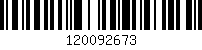
\includegraphics[scale=0.5]{thk11-barcode.png}
\end{center}


               

\thispagestyle{empty}

\begin{center}
    {\LARGE\bf Acknowledgements}
\end{center}

I would like to thank myself for all my hard work. 

Cheers. 
 % Acknowledgements
\thispagestyle{empty}

\begin{center}
    {\LARGE\bf Abstract}
\end{center}

The aim for this project was to provide an alternative android native application to the current
Access Aber web application, while also improving on the groundwork laid out by the initial
work. This was done due to the help it can provide to users who are visiting the University as
well as providing at least some assistance to those with disabilities. Aberystwyths campus can be
a hard place to navigate and the benefits provided from a mobile device can benefit users to a large
degree.
The application was developed for the android OS using the Android Studio IDE and relies
heavily upon the Google Maps API. It provides a range of services to the user, some of which
were brought over from the existing application and improved, some new. These include route
finding around campus, user refined display’s of building locations, route plotter with application
compatible outputs and a location based help system.
This dissertation covers the original analysis, requirements, design and implementation of the
project as well as details on the testing and design decision made throughout the development.
The conclusion is an android application which met its original requirements specification and
adds further complexity to the initial web version of the project. This includes route grading and
the representation of this along with an extendable solution to route finding using Google Maps
and graph searching techniques.                 % Abstract

\pagenumbering{roman}
\pagestyle{fancy}
\fancyhead{}
\fancyfoot[C]{\thepage}
\renewcommand{\headrulewidth}{0 pt}
\renewcommand{\chaptermark}[1]{\markboth{#1}{}}

\tableofcontents  
\newpage
\listoffigures
\newpage 
\listoftables
\newpage

% Set up page numbering
\pagenumbering{arabic}

\setchapterheaderfooter

% include the chapters
\chapter{Background \& Objectives}

\section{Background}
\subsection{Background and Preparation}
Background research was compromised of analysing existing systems like the original Access Aber, previous work completed by the developer that used map technology within Android and general research into the map technology to gather a strong understanding of exactly what was possible.

A majority of time was spent analysing Access Aber and the currently existing criticisms of it, a lot of the problems were clear without the user feedback that had been provided but some criticisms were more subtle but easy to understand like how the application provides no main menu as such causing the user to feel lost from the start. It was also obvious that at a technical level, the included features were not overly complex, at least not to complete on the Android platform. Due to the application originally being developed on a system which allowed it to be run both on iOS and Android there probably were limitations from both sides which leads to having to develop around the weak elements in both platforms. As stated developing for a single platform should help us avoid these problems while also giving us the ability to take advantage of what is there. Due to this a large amount of research was completed into both UI design within Android as well as the technical benefits both Open Street Maps and Google Maps could provide the development. 

Research was also completed into exactly how the mesh of locations would be created and represented, within the design specification it was concluded that a searchable graph was a possible solution and one worth researching further. This also meant analysing how other existing applications had mapped roads to graphs and the general area of map representation. While this gave a fair amount of answers further decisions needed to be made on both how to search the constructed graph and how to make it an extendible system for future additions. This was one of the main conditions brought up in meetings with the original 'customers' of the Access Aber application, it had to be functional after the initial developers had left. It was also described that it would be beneficial for the application to be developed in such a way that a possible future development that involved a central file store of the information for ranging versions of the application. Due to this further research was done on how we could leave the application in such a way that it facilitated the addition of this feature possibly without using it upon the current cycles completion. 

Past work by the developer was also analysed for anything of use that may come out of it, the application analysed was proven to have functional working code and as such was a place where possible solutions could be found. This included implementation of maps in an Android environment, the logging of a route which is something that has been previously outlined as a key requirement and a fair amount of small features relating the monitoring of a users location and the information which can be gathered from that. Most information gathered from this however was fairly irrelevant, it was decided it was not the best place for referencing in future. 

Finally the Android API and several Android libraries were examined for the benefits they could provide the development with, along with the search for several features that had already been selected for inclusion within the application. This ranged from simple research on Expandable List Views to research on the best way to present the application in an intuitive way, a lot of factors were gathered from the original feedback which guided a lot of the research. While a slide function for the screens was visually appealing the possibility of it confusing users was something that removed it as a possibility very quickly. Research was also performed into Google's Material Design program, a set of guidelines for good design within the Android environment. It contained a large amount of information relating to designing professional and good looking applications, while the information was too much to be fully applied in the projects time line some key ideas were taken from it relating to the design of elements within an application and general theme layout. Furthermore some sites were analysed for basic colour themes and how to implement a simplistic design without it looking unprofessional.
\subsection{Interests}
This project has been chosen due to a variety of reasons, revolving around both the developers interests and the possibility of the project leading to something that can have real world influences. The main source of interest is that the project allows for a development environment that takes input from the real world, mobile devices are of a great deal of interest to the developer due to the data that can be gathered from them and the manipulation of this data. Mobile devices are steadily changing the way we live, with applications that not only help us find where to go but tell us what we can do when we get there. Where other people have liked and even what is best suited to us based on past choices we have made and the device has noted. While some systems outside of mobile development clearly have massive real world influences it is felt by the developer that the easy entry and possibilities provided with mobile development make it one of the most accessible and revolutionary platforms.

With the application in concern providing information to the user it also means we can filter what information is shown based on user details. If the user says i cannot manoeuvre stairs for whatever reason, we could implement a function to provide paths with no stairs, this could obviously be expanded to include searching based on a range of filters. This could also be condensed down to a single graph, with different links becoming available with different information. This kind of possibility is what makes mobile such an interesting platform, not only can we show a map and a route through it, we can then guide a user through it, even ask them for information regarding it once they are done. Possibilities provided are wide and interesting, with so many choices available the future of the application is impossible to predict because of the many paths it could possibly follow.

Another source of interest is the real effect this application could have for an organisation such as Aberystwyth University, the confusing and difficult to traverse campus is not a problem that can be resolved easily. With everything on campus set in stone it is simply not possible to move buildings and locations around. However with technology we can facilitate the use of campus without any physical additions to it at all. This means we can change the physical use of something with technology that does not itself directly effect or control the environment it is deployed in. An interesting possibility would be to examine users manoeuvring of campus before the application is introduced and afterwards, as well as the effect it has on how comfortable disabled users feel on campus. With the application very literally changing the way a user traverses the campus it is possible that some of the more unused walkways could become more travelled due to their inclusion in the application. Further research will have to be done on most effective travel paths around campus, it is likely that the ones currently most travelled are the quickest but that is not definite. 
\section{Analysis}
A broad analysis of the problem with the currently existing Access Aber application is that while it provides solutions, they are long, problematic and make the user follow a convoluted process that may not be obvious to the common person, the exact person we are aiming to help with the application. A prime example of the problems posed is in the route finding within the application, it exists but requires the user to scroll through a huge list of possible routes and then takes them to a summary screen before finally letting the user see the route they need to walk. There are some very obvious, stand out ways, that this can be improved including the implementation of simple features like drop-down boxes for destinations and the removal of the summary screen. 

Most of the problems in the application come from simple solutions to more complex problems, simple in the way that they do not fully cover the problem or provide a real benefit to the system. This appears throughout the application and based on the information provided seems to have been caused by the short time period it was developed in. One aim for this project is to provide a much more polished result with each problem solved properly rather than meeting requirements with a 'it will suffice' mentality. 

Access Aber's initial form will be treated as a kind of groundwork for development, while no code will actually be taken from it the features will be adapted and built upon. This way we can build not only a port of the application to Android we can build a better version which in turn can act as ground work for any future work on the project, be it with the Android application or another new version on another platform. Having this groundwork and the feedback on it means that the some of the problems that need fixing are already highlighted for us, while the time line of the project may not be long enough for some of the features to be fixed most can at least be addressed. 

A step by step guide which details various information such as major features and activities can be seen in the Design Specification (Section 2). The following requirements are what has been decided as key to the success of the application, they have been selected due to either their use to the user or the fact that they have always been included in the project and these aim to be improved versions. 
\subsection{Breakdown of Requirements}
After much analysis the problem has been broken down into a set of requirements, some of the process to arriving at this point can be found in both the Requirements specification with further information in the Design Specification, however the reasoning will be fully discussed here. Each requirement will serve as a benchmark for the project, requirements were set as realistically as possible considering the time given and the work that needs to be completed. 
\subsubsection{Route Finding}
Route finding is seen as by far the major feature within the application, not only is it the most technologically advanced it is also the most useful for our prospective users. As detailed, a graph system had been highlighted as the best way to achieve a representation of campus for us to apply a search algorithm to, with Breadth First Search (BFS from now) seen as a possible solution for the time being. This feature also has some planned extensions to it, firstly the path shown to the user should contain extra information pertaining to the path. This includes information about the difficulty of the route and features along the route such as stairs, it would be beneficial to have information for separate segments beyond their rating but this is a stretch goal and not something should realistically be expected. Due to the expected structure of the graph the implementation of displaying rating of segments within the paths should be attainable, with large routes being made up of many links between nodes it is almost to be expected in a system such as this. 

It is key that the route finding solution be easily expandable, this is due to the maintainability of the application being key to its success. There is no guarantee that the original developer will be around for future expanding if the application is deemed fit for purpose and further developed, due to this it must be possible for the adding of new locations to be possible. An ideal solution would use a central file store to pull location information from, however the problem here which has been previously covered is that there is no guarantee the user has access to internet when using the application. Due to this a sufficient solution should see that the extending of route finding should be achievable by a novice programmer, ideally a common user if they are provided with clear instructions. A set of guidelines should be produced if the project is taken further. 

A further stretch goal would be an implementation of route finding based on a sort of filter, whether this be a routes rating or features on the route. A current rough idea of this can be found in the Design Specification (2.1.1), this highlights the idea of using a separate graph altogether, this way if we make the search algorithm so that all it needs is a set of files in a set way we can have a variety of graphs present within the application. An ideal solution would use a consolidated graph, with different routes between different Nodes being considered, however this is seen as problematic in the current time frame. 

A final possible addition, though not likely to be achievable in the time frame, is to provide access from anywhere to somewhere on campus. This means having a user be guided into the graph from areas outside of it, meaning dynamic routes would have to be created. Initial research shows this could be possible using the Google Directions API however it is likely that with other development ongoing this is likely to be feature developed outside of the initial time frame. However the use of this feature would be a real benefit for the application, a simplistic solution would have the user guided to the nearest node and then the search algorithm would take it from there. It is even possible that in future the whole graph would be replaced with the Directions API, this however would require the user to have access to the internet at all times and it is simply something that cannot be guaranteed. Due to this the hard coded graph and search related to the graph is likely to be present for the lifetime of the application due to the required off line capabilities. 
\subsubsection{Route Plotting}
This desired features comes as a result of the original meetings, the 'customers' were unhappy with the current system of plotting routes, which were all done manually.  Part of the solution is already achieved through the use of a graph, a location only needs to be linked to one other to have a route available to anywhere on the graph. However this should be further developed for the application to be seen as fully functional. The application should include a feature that lets a user log a route and have it printed out to a file compatible with the current route finding solution, this way the person responsible for the future maintenance of the application can visualize a route before they add it to the current system. A route should be able to be visualized while it is being created, so that the user is not blindly adding points. GPS co ordinates received from some devices can be far from where the actual user is. Functionality within the Google Maps API allows us to show the user where the phone thinks they are, this should help them plot accurate points. 

The output file, the files used by the route finder, should also be human readable. This requirement is not as key as the others but should be achievable as the file reader will be coded for this exact purpose. Having a human readable file provides various benefits, mostly that of being easily editable by anyone who wishes to change information in the future. Its negatives are few, while a non human readable may be able to be smaller the benefits time wise will be minimal. This also means that route plotting using the in built feature is not required, files can still be made by hand due to the standard format to be laid out. 

Finally the Route Plotter should provide a grading for the route that has been laid out by the user. This is the grading that will be displayed by colour on the route finder, while the initial rating is likely to be numerical this will be translated into the red, amber, green system that has been mentioned in the previous meetings. Having this easily identifiable system provides the user with a sense of understanding without having to state the feature on screen and cause cluttering in the UI. Ideally the route plotter will take into account cumulative distance, steps on the route and elevation. However after initial research elevation is not only sometimes unreliable but a complex overall problem, to do with both the misleading information it can provide and the problems in finding elevation. However an ideal solution would take all three factors into account fairly.  
\subsubsection{Building Display}
Building display is a feature currently implemented fairly well within the original application and is something we can mostly just adapt, however there are improvements that can be made, mostly found due to the user feedback. This feature should allow for users to highlight building types and have them displayed on a map of campus, this way a user can browse around what they want rather than have to try and guess where certain areas of interest are. A user should also have there location displayed to them so that they know where a building is in relation to them.

One criticism that has come from the user feedback is that sometimes the display can be less than clear, this includes building departments sometimes not being named and just a general lack of clarity. A good example is buildings named after people just having the persons name, for example 'Hugh Owen'. Problems like this should be fixed for the requirement to be met. Again a facility for easy addition to this feature should be added, preferable through on device files for the time being due to the previously highlighted problems with a central file store. 
\subsubsection{Location Based Help}
Location Based help is seen as the easiest implemented feature, something that the web application also currently lacks. It is seen as more of a test than the other features which seem solid and long lasting, the resources available to the University may not be able to facilitate the full deployment this feature may require.  In short the feature should be able to provide the user with the details of the closest person who could provide help, currently this is limited to the three libraries which have their accessibility officers details listed on line. However other buildings will have persons responsible for this its just their details need to be retrieved from either the departments the buildings are home to or the University.

A possible change to this implementation is the addition of porters to the help listed, if all three locations are too far away, a porters could be contacted instead. However a dialouge would have to be opened up with the University over whether they find these practices acceptable. For this application they will be implemented as a proof of concept. But in future they could either be removed or only available on set days when the demand for the services is expected.

A further idea which would have to be completed after the projects time line is to have two separate applications on open days, one for visitors which is the one being developed in this project and one for the helpers hired by the University for the day. The application provided to the Helpers would be linked with the Help function shown here, on Open Days the application would take a users request for help and give one of the Helpers their location. By doing this we provide a way for confused users or just users looking for a personal guide a way to acquire both of those. This could be completed in a fairly short amount of time with a developer who has experience with what is likely to be a PHP and SQL back end. However this is a future plan and not something to be expected from this application.  
\subsubsection{UI Design}
Interface Design itself contains a set of requirements that can be mostly boiled down to one key aspect - an intuitive interface for the User. Currently there are several problems with the existing interface that can be fixed fairly easily, like the lack of a menu and unclear buttons. However a fully intuitive interface will take time to develop, testing and a good amount of inspiration from other sources. Within this project it is the aim to have a clean, practical layout that most users can just pick up and use without and previous knowledge of the layout. By doing this we guarantee less confusion and problem free use of the project, it also means we would get less users wanting to use the Help feature which if implemented would be a big bonus for the University and development team. 

This requirement can also be broken down into further aspects than just 'intuitive design'. Firstly the theme used within the application must be consistent without, it would also be beneficial if it coincided with the Universities colours of yellow and purple but this will not be treated as a requirement as of now, due to the restrictions it places on the development team. Buttons should be labelled clearly with reactive designs to users touch, there are few issues worse than no responsive buttons that do not give the user the feeling of actually starting a process. The design should also be simple with non overpowering colours, we want the user to feel comfortable and a confusing sea of bright colours over a map is not a good way to achieve this.

Future goals could be varied colour schemes based on colour blindness, with the application aiming to help those with disabilities ignoring those with colour blindness is a large oversight and is something that should be considered in the future. It may be possible to implemented in this version and is something that should be strived for. Another feature which is seen as a key requirement is Welsh language support. With the application being developed for a Welsh University the inclusion of this is key, current research points to this being more than possible despite Android not natively supporting Welsh as a current locale. This can be programmed in however meaning it should be achieved in the current time frame. 
\subsection{Itemized Requirements}
Following is the list of requirements for the project, some requirements can also be seen in the requirements document however these detail a more up to date version with more focus on smaller details.

\begin{itemize}
	\item FR1 - Route Finding - Guiding a User around campus, including the display of route grading and a no steps graph.
	\item FR2 - Route Plotting - Users must be able to plot their own routes around campus and print them to an application compatible file.
	\item FR3 - Location Based Help - Provide details of possible help available, possibly include the addition of contacting porters. 
	\item FR4 - Building Display - A display of related buildings to be filtered by the user, contains accurate information on buildings and the departments in them. 
	\item FR5 - Multi Lingual Support - Welsh translations provided in the application and a user choice on what language they would like. 
	\item FR6 - A clean and simplistic UI with clearly labelled buttons and a mostly responsive design, possibly including colour blind themes.
\end{itemize}
\section{Process}
For the development of this project an adapted Feature Driven Development style was used, taking a lot of ideas from FDD but still changing the development style slightly. To begin with an overall design was specified in the Design Specification document, this included the design for the entire program. It covers a range of information, including an overall model which is the starting step of FDD, information on the key expected algorithms and key classes to be expected. 

A type of feature list was also developed within the Requirements specification, while more verbose than may be expected with a feature list it still detailed the features expected and the finer details to be included. This document is more abstract and tends to not focus on the actual technology too much, just what is desired from the program itself. The Requirements Specification also outlines key attributes that must be included within the application, this includes details on the maintainability of the project and possible choices for future expansion. 

Planning by feature was something that was mainly omitted from the process, due to using a single developer all of the work load fell onto the single person. However milestones were still set for iterations of every three days or so, estimations on progress were made. A set feature was either expected to be completed or a quantifiable progress. Some difficult areas of the project led to targets not being met but overall the model provides a target to aim for in a given time frame. 

Designing by feature was also a process that only partly took place, due to the majority of design happening near the start of the project a majority of the time the design by feature process involved the editing of existing documentation to better reflect what was now expected. As development continues designs for future features tend to change a lot due to shifting scope and time restrictions either becoming tighter or allowing more polished features. Having a design from the start meant that development could continually take place without major breaks for planning out a feature, this meant that once the application hit its main development stage it got quicker to develop due to a familiarity with the code base and the final image of the software becoming clearer as time progressed. 

A lot of time after the initial design was completed was spent on development, this meant progress and development tended to be quick. Building by feature meant the application had modules added to it weekly, creating a progress that was quantifiable. This development technique was decided to be the best process for a smooth development period. It also helped that the application could clearly be visualized as having several different branches, most of which did not rely on one another. After development was finished tests were performed, both code wise and with the application itself ensuring the code worked as expected. It was also important to test that the code was expandable and that the plans for the future could be included in the way that was highlighted within the Design and Requirements specification. \\
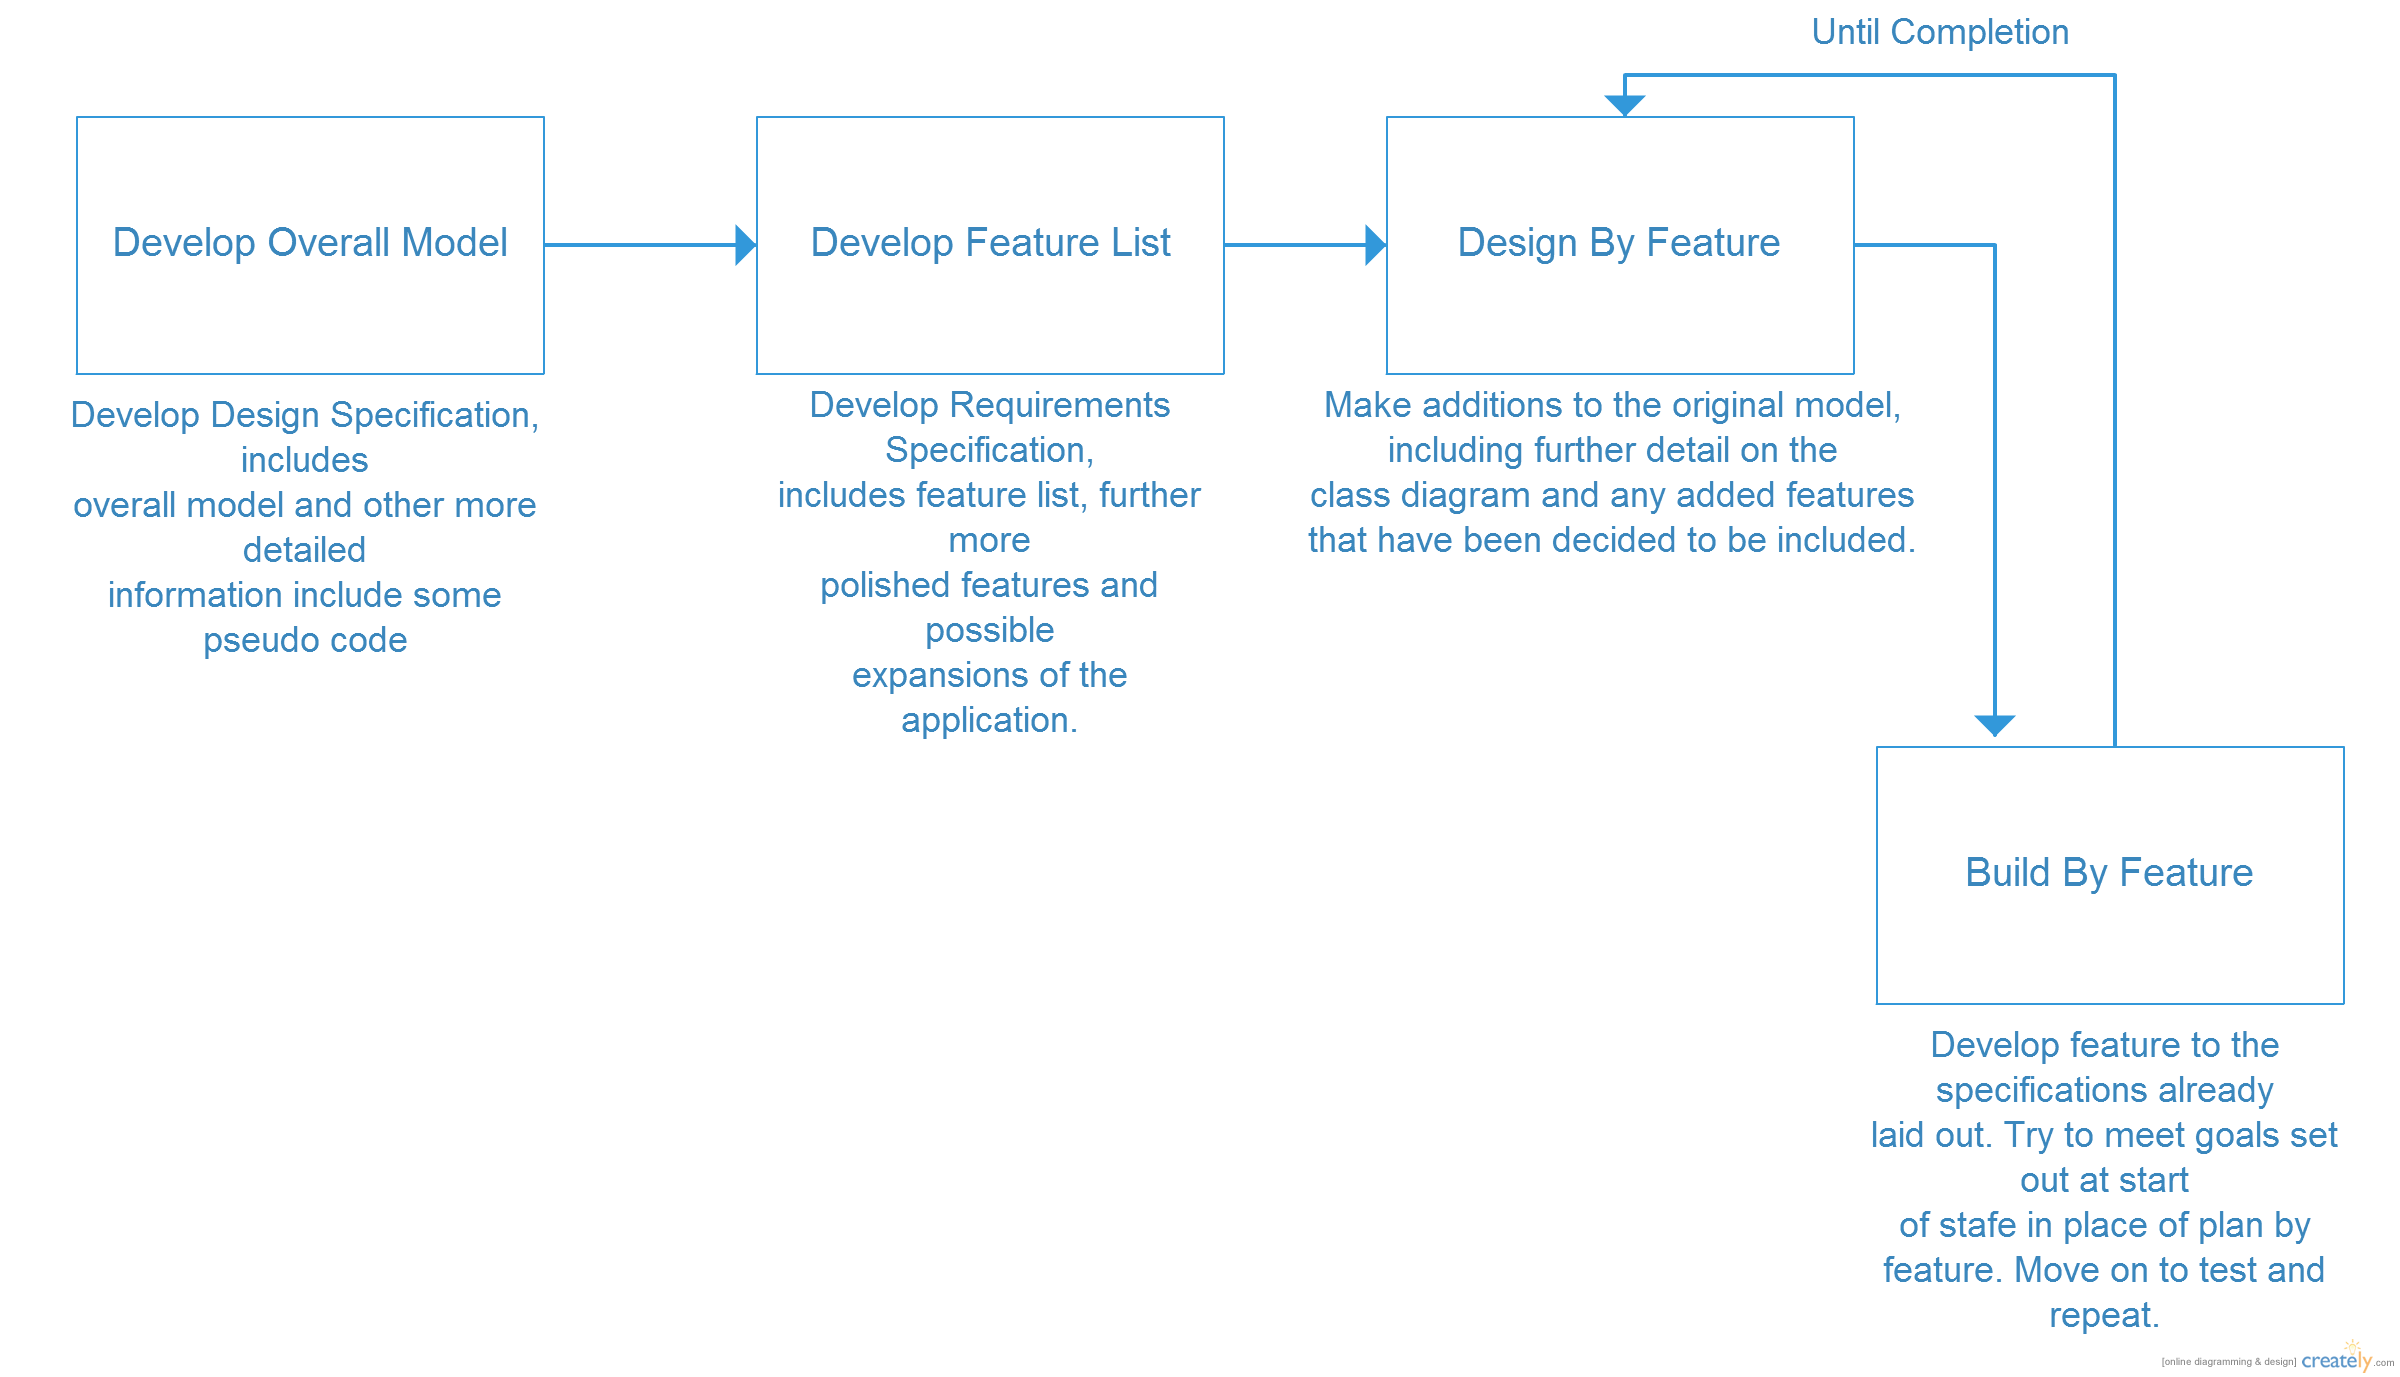
\includegraphics[scale=0.2]{Chapter1/process.png}\\

%\addcontentsline{toc}{chapter}{Development Process}
\chapter{Design}
The following section will cover the final design of the project, initial design can be seen in the Design Specification. The original design was completed when only a small amount of research had been completed and not all avenues of interest had been explored. Due to this good comparisons can be made between the two making it easy to highlight the areas of the design where large changes were made. The design covered is the cumulative output of the Design by Feature element in the process. This means some changes were still made during the implementation phase but those will be discussed in the relevant section.
 \newpage
\section{Support and Development Tools}
\subsection{Development Environment}
During the initial phases of development and prototyping Eclipse and the Android Development Tools plug in were used to help develop the application, this was due to the developer having experience with this platform and the code being sampled from other projects was also built within this platform. However not long after initial prototyping and tech spikes had started to take place the decision was made to swap over to Android Studio and develop from there. Most of the decision comes down to personal preference but there are definitely good justifications to swap, personal preferences included appearance and responsiveness as well as easy to use features such as inbuilt git support and intuitive interfaces. 

One major contributing factor was the initial hassle in updating the ADT to their latest versions, this process alone took hours of research and tinkering to get fully working. During this time it was discovered that Google had stopped support for Eclipse ADT and would be focusing on the now fully released Android Studio. A decision was made, based on the advice from the Android API and other sites, to move over to Android Studio as it would quickly surpass Eclipse ADT with some features already being far more helpful.

One key feature that was seen as a bonus when compared to ADT was the interface editor, while this is present in the Eclipse version the process in Android Studio seemed much more responsive and seemed to give a clearer idea of what XML was being written to support the graphical changes. While nearly all interface development was completed using pure XML sometimes moving elements using the graphical layout gave good suggestions on exactly how a set layout could be achieved. While the code produced by this could sometimes be messy and convoluted it could also be cleaned up and improved. 

Some of the choice to move over was also personal opinion of the developers, with so much time having to be spent in the IDE it had to be at least a suitable experience. After past experience with Eclipse and ADT causing issues due to freezing and crashes the supposedly much more stable AS was worth adapting to. AS also seemed to provide a much fuller auto complete feature, suggestions would be made sometimes within a single letter of a word being typed out, normally correct suggestions. Once used to this process code could be written up slightly quicker making the experience overall more enjoyable and productive. Overall the experience with AS was that it was far less cumbersome and much more enjoyable than  Eclipse ADT. While currently there may not be huge differences the ones included were very helpful, the implementation of Gradle meant single lines could be used for the inclusion of dependencies and possible libraries. Easy inclusion like this meant that it was a lot more appealing to try out libraries and see what they added to the project. While Gradle provides many benefits not all were made of use within the project. 

A final reason for choosing Android Studio was that after seeing various comments on Android discussion boards it became obvious that it was quickly becoming the industry standard, unsurprisingly due to the lack of support for Eclipse ADT. Adapting to AS seemed the most logical decision, made easier by its sleek appearance and performance. 
\subsection{Version Control}
Version control was an easy problem to solve, as standard GitHub was used to upload versions of code and documents allowing the history of changes to be made and development easily tracked. It also meant that in future the project could easily be open sourced through the changing of the privacy settings on the repository. Using GitHub also meant that even when on the move developers could check the code base through the website to see if potential solutions could possibly be implemented. 

One alternative to GitHub which was considered was BitBucket, BitBucket provided unlimited private repositories and a desktop client which could have been of a fair amount of use. However looking at reviews and the general design, the developer decided that while there were benefits in using BitBucket over GitHub, they did not really apply to the project due to its small size. In future if the project was undertaken by a larger team, or the developer was part of a larger team for a seperate project, BitBucket could be heavily considered due to its unlimited private repositories as standard. 

Having the code stored off site as such also provides a range of benefits to the developers. It mostly frees up the developers to not worry about breaking any code, back ups from various times are all available with the ability to roll back to them with minimal effort. It also meant that the code was always safe, once the code had been moved to the GitHub servers its available for the future, no need to worry about corrupt drives or other similar issues. 

GitHub also provides a simple and easy to use graphical interface as an alternative to the command line interface. This interface was sufficient for the project being completed with only a few clicks allowing for the new code base to be committed and pushed to the on line version. While this may not seem a major benefit it still freed up some time and overall made the task of version control slightly more enjoyable. 

An alternative to using GitHub for version control and code backup was either storing backups externally using flash drives and external hard drives or using the file store given to students by the University. However the benefits provided by these were more than covered by what GitHub provided, it was also decided that there was a minimal chance of losing any data stored through GitHub while it was possible that we could lose access to the file store for prolonged periods of time without prior notice. This has been previously experienced and was not something that the developer wanted to risk.

Without version control it would be possible to completely lose track of what had changed, as well as losing the project as a whole. Storing everything locally is extremely bad practice as any amount of extenuating circumstances could lead to either the loss or damage of the computer that the information is stored on. Furthermore GitHub provided statistics on when most commits were made and exactly what was committed, this allowed for estimations on not only how long a feature would take to develop based on what time had currently passed, but how long a future feature would take based on its complexity compared to past features. This meant that during development a fairly tight schedule of development was set out and mainly adhered by.
\section{Overall Architecture}
Initial design for the project was very broad becoming more focused over development time. With the Design Specification it is possible to see the first properly documented steps in preparing for the development time within the project, however other initial steps were taken first to help build a design from. At the start of the project a very abstract set of diagrams were drawn up to describe the desired boundaries for the project, this was mainly as a guide for further development but aids in demonstrating the vision of the project from the start. While these were drawn up on paper the digitized version will follow, it can be seen that the diagram is essentially a flow diagram that only involves the Activities used in the Android application. No screen details are given just the links between them, this has changed significantly over development but the basic blocks can be seen here. A link can be seen between Route Plotter and Route Display, this was to represent the output from one being compatible with the other. \\
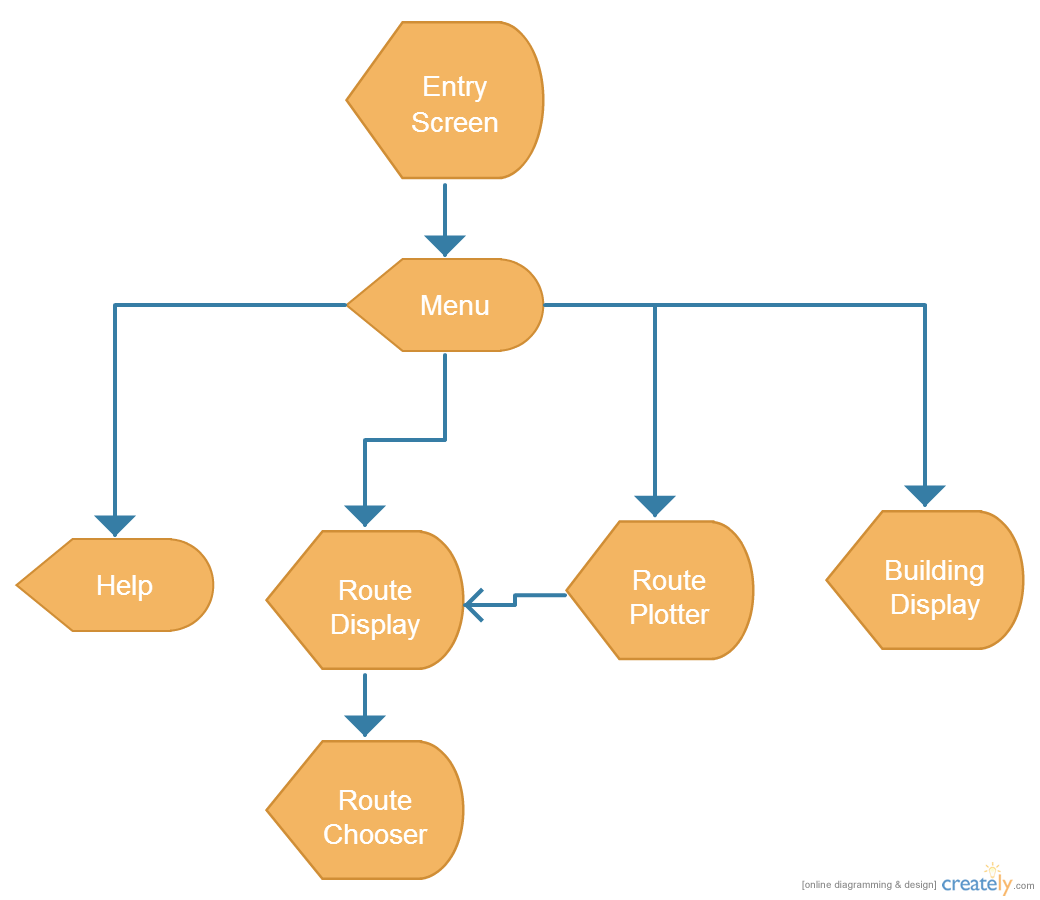
\includegraphics[scale=0.4]{Chapter2/screen.png}
\newpage
\subsection{Class Diagram and Justification}
The final Class Diagram represents what was thought to be the final representation before the Build Feature segment in the process, during implementation some changes were made but the class diagram is a good representation of how the program actually works. Justification of the design will follow with diagram afterwards. 
\subsubsection{Justification}
In this diagram the Menu Activity serves as an entry point into the program, in production it was always intended to have a simple screen before this, however for the case of the class diagram representing it is non informative as it does nothing but show a logo, it is not essential. Within the program the simplest function is the Help Activity, this Activity is created through a button click within the Menu Activity. Within the Activity is an ArrayList of Place, a Place is a simple representation of a location on the planet and is used repeatedly throughout the code for varying uses, in this case it represents a set of potential helpers. Within the Place objects a persons name is the Name variable and their details as the Description, these helper points will be loaded in from a file and then manipulated with methods within the Help function, these methods will load the points, sort them and display the closest one to the user. 

One of the possible alternative options that was considered here was the inclusion of a Person object and instead of a Place object have a Building object which could have an array of People. However the choice was made to have people represented as places, this was due to an effort to simplify the programs structure. With Place being used for varying reasons without it being overcomplicated no need was seen to include two separate classes. If all places were buildings it would have been considered a worthwhile effort, however Places are also used to represent points on a Route and they are not always Buildings. As the program stands it is sufficient to have one class represent people and places, including buildings, however in future if more expansions are completed this may change. One area which may change this is the inclusion of porters or open day helpers in the category of 'Help'. Huge changes would need to be made to the structure of the program to support this feature however, including external hardware to act as a middle man between the application and the 'Help' on hand. 

Slightly more complicated is the building display feature which is made up of several classes including the reuse of the Place class. In this case the Place class is used to represent a set of locations relating to a category defined by the user, this ranges from facilities on campus to lecture theatres. Within the Map Activities onCreate method is the code to render different views based on the request of the user, as the Map class is used to represent both route plotting and building display. While the same XML should be used, methods within the Activity should manipulate it, acting as a type of presenter. A choice which arose in the implementation of this is whether it would just be simpler to have two different Activities for the tasks, however with how little they both used and the fact both tasks used a map fragment it was realised it may be just as effective to use the same Activity. 

With the Building Display function being used the class Place is now used to represent buildings, making use of their 'type' variable. Types are chosen from an Enumeration class which limits the pool of values, while it would have been possible to just use Strings the Enumeration removes the chance of mislabelling a buildings type as the pool of values are the only acceptable choices. This makes it easy to error check for erroneous data on the load in of the buildings, having the added error checking assists in the robustness of the application. 

All of the data loaded in is then used within the Map Activity, within the Activity are the methods to handle the representing of a set of locations based on their type variable. With us having a handle to all of the locations the displaying of them is easy to represent with the Google Map, using the showByType method and passing it the locations and a desired help will suffice in rendering any of the types we want. It is best to do this on a button click, likely from a pop up menu. By doing this we can pass the String used in the menu and have that serve as the type, all this requires is correct labelling of the items in the menu. We can then cycle throughout the data object and show the ones we need as marker objects on the map, showing both their name and description as was set as a requirement due to past user feedback. It is debatable whether all previous displayed locations should be wiped after a new category is selected, or whether a user should instead be able to choose a set of categories for display. To begin with a user will only be able to select one category at a time but this could change with future user feedback. 

One of the more complex features which has involved a lot of design decisions has been the inclusion of the Route plotter feature, due to the complexity of route representation on a map many ideal features are simply impossible to implement in an ideal and functional way, some of this is down the the unreliable nature of near perfect accuracy from GPS. When a user requests to plot a route they are originally brought to the RouteDataEntry Activity, this is a simple activity which will let the user put in anything they like as the start point, to help with adding new original locations, but limit them to entering a pre existing location on the graph as a destination, thus ensuring a fully connected and traversable graph. It should also allow for the user to specify whether the route is for the step free or standard graph. 

Once the user has completed entering the required data, the Map Activity should render itself based on the users request. In this case, the display button will be replaced with one which contains a menu for the methods required to accurately plot a route. A problem encountered in prototyping is the creation of a Place for the Route object based on a user's location, this has been down to the fact that GPS co ordinates are not always accurate, especially in built up areas. To combat this, it has been decided that a point will only be added to a Route on the user's command, with the user's location being displayed on the Map object. An alternative option would be to have the device log a point automatically every five seconds, however this caused many 'off' locations to be included. With the inclusion of these off locations, an almost jagged path was produced compared to what user defined logging times provides. 

To aid with the visual representation of a route each time a user logs a point after the first a poly line should be used to represent the traversed path. This should be done using the connectPoints method which takes two Place objects from the Route. Having a visual representation provides much better results than having a user blindly plot a path, it also means that combined with a user being able to see there location they can accurately tell the line that will be drawn before it is. A small incremental counter should also be included within the XML file to log the steps encountered on a route. Once a user has finished logging the path they wish to add to the graph they should be able to print a program compatible file. This is handled by the printFile function which takes the completed Route, within this a variety of functions are called resulting in a final printed file. Methods called from within the printFile will be calcDistance to return the final distance between points and the calcGrade function to return the final grading of the route. Grading will be done by normalizing the total distance and steps to the same scale to figure out there 'rating'. A set of boundaries will be used to define the rating.

One major difference between this design and the previous included within the Design Specification is the change of what the Map object considers its route. Initially it was implemented so that the Activity stored information considering the grading, start and destination along with an ArrayList of Place. However it was recognised that this is a bad representation considering we already have a working Route object used within route finding. If the object represents a route in one part of the application but not another it could be considered confusing for future developers. An additional change is the inclusion of the data entry Activity, this was an oversight in the initial design and something that has been fixed in this version. 

Route Finding within the program will be by far the most complex feature to implement. This is down to a variety of reasons including having to implement a search technique which performs reliably. Before any graph analysis is done the user should select
 what graph they want to use by making a choice between what is represented as two separate features. They should be asked if they want standard routes or easier routes, shown as a 'no step' option. While this appears as two separate features all it should realistically change is the graph used for search and traversal, this also opens up the possibility of having more than two graphs in future however more complex and effective solutions could be included. 
 
Representation of a Route is something that a fair amount of thought has been put into before development, due to the importance of being accurate. Within the proposed system a Route is essentially details of two connecting Nodes on a graph and the link between them. As it stands the link between the nodes is represented as a set of GPS co ordinates which when plotted in order describe a set of destinations which lead to the final location. By doing this we help represent curves in the links between nodes. In this design a links weight is represented as a grading which is set based on criteria laid out in the Route Plotter Activity. Searching could be completed based on route grading but may be outside of the scope on this project. 
 
After the choice of what type of routes they want returned the user should be taken to a Map object with a button which will take them to the RouteChoose Activity. This Activity will contain two expandable list views populated through a file within the relevant assets folder. Another option would have been hard coded values but these do not provide the expandability felt necessary. Once a user has chosen their start and destination they should be taken back to the Route Display Activity to see the route, before this happens the route will be found using a search technique within the Route Choose Activity. This method will return what is actually an array of Routes, by doing this we have segments to our routes and can manipulate its colour in segments allowing for the display of different colours based on the difficulty of small sections.

A choice which arises here is exactly how to search for a Route through the graph. Currently it has been decided that a simple Breadth First Search will be implemented. By doing this we can move through the graph and continue until we have found a small route which ends in the destination and build backwards from there. In future, if the graph expands to be quite large, it is suggested another more complex search technique be included if time is not found within this project. 

Once a user is returned to the Route Display a set of methods will be run to handle displaying the routes. First the Route array will be pulled out of the Intent returned from the Chooser Activity, this will then be set using the setRoute method which will in turn use the loadFile method to get access to routes stored within the programs assets. As previously stated the Assets folder accessed will depends on the type of route finding the user has requested. A small window should also display the steps on a route and other information including the distance that has to be covered. 


\begin{sidewaysfigure}
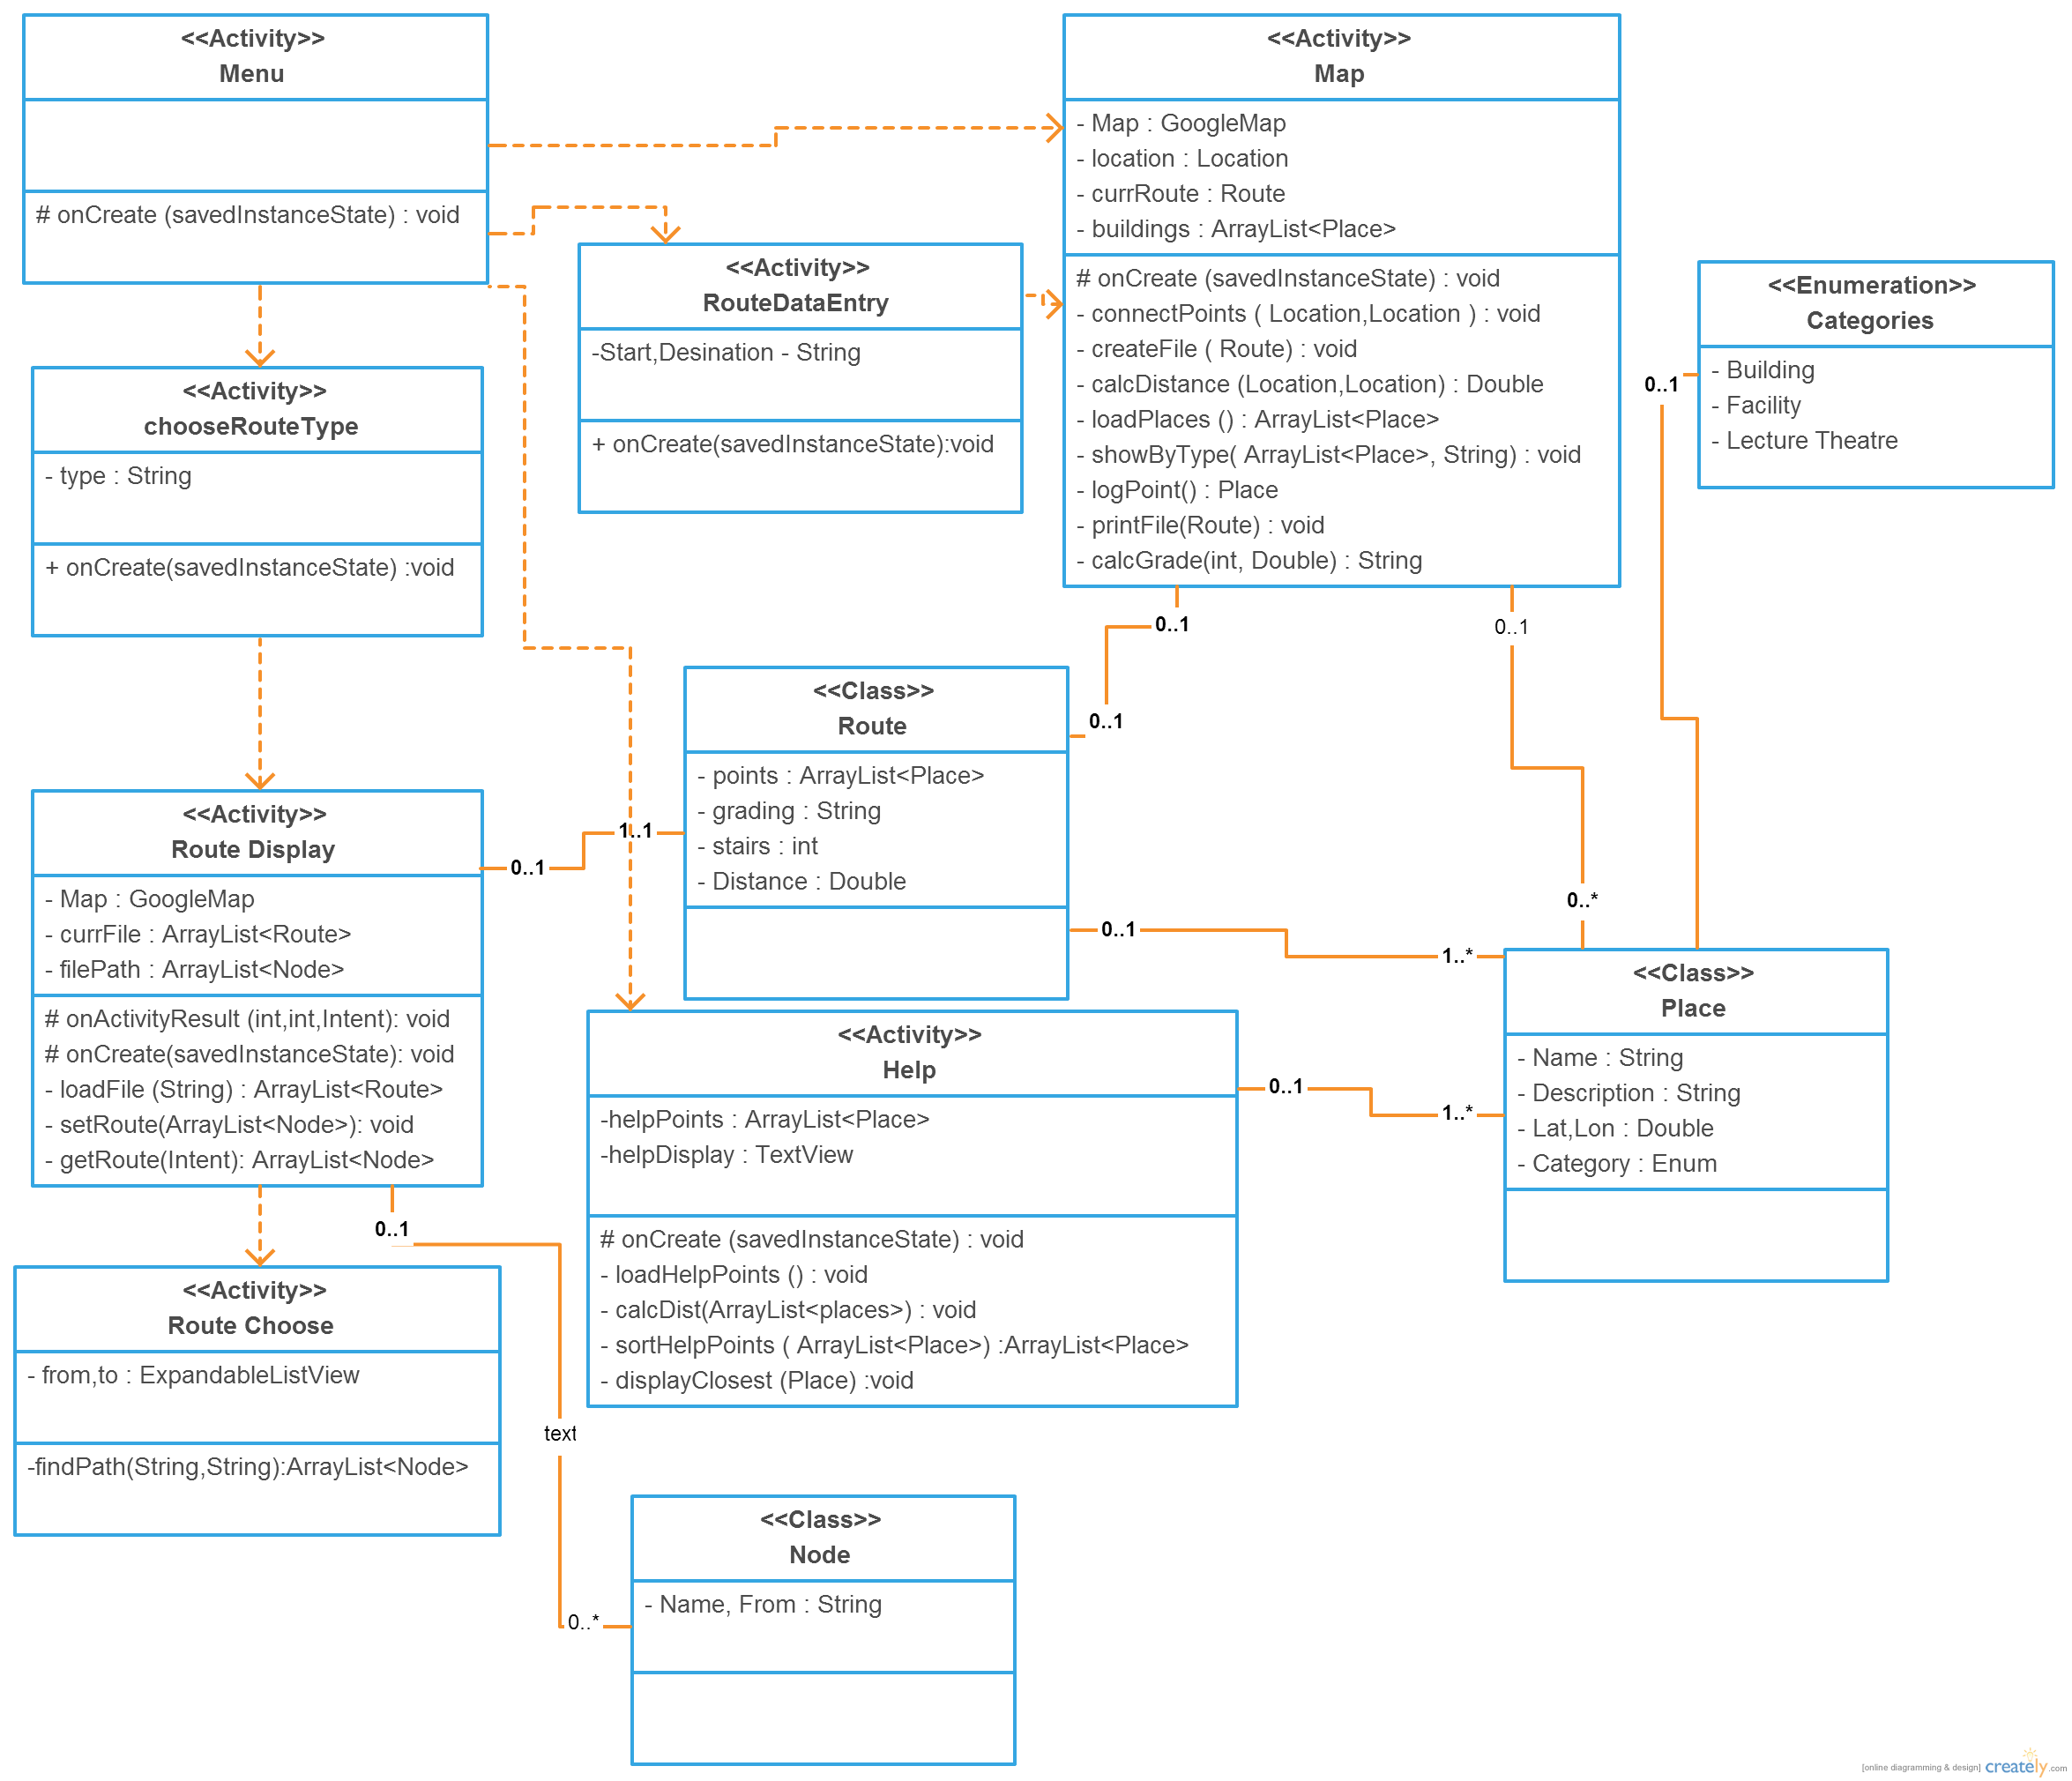
\includegraphics[scale=0.28]{Chapter2/class.png} \\
\end{sidewaysfigure}
\newpage
\section{Application Flow}
With this application most users will be first time users, it is not likely it will be repeatedly used by someone after they are used to the campus. With this in mind it becomes clear that good UI design is important, along with logical flow of the application. A basic flow of screens can be seen in 2.2 however it describes a very broad series of events. In this section a detailed flow of data and screens will be detailed to help with the implementation phase. The diagrams following and the textual descriptions should be used as a framework to build around. 
\subsection{Overall Justification}
A similar diagram to this can be seen in the Design Specification, section 4.1, however this revised version details updates including additions of screens and specific details on what should be contained within some algorithms and the alternative considered. 

One of the changes included within this diagram is the inclusion of the Route Data Entry Activity, this is used for the user to enter the start and destination of the route they are plotting. While this obviously needed to be included it was not within the original diagram, a major decision revolving around this screen is exactly where it should be placed within the application. It is viable to include the screen between either the choice and the plotting screen, or have it used after the user chooses to upload the route they are currently plotting. It has been decided to include this before the user plots anything, this is due to to the idea that the user should provide broad details like the start and end before adding information about the detailed route. It follow a logical progression this way. 

After these details are chosen the $addInfo()$ and  $renderPlotter()$ functions are run. These should actually be run in the $onCreate()$ within the Map Activity. This way the information added in can be accessed from the past Intent to detail what to render and what to name the route. This also applies for the $renderDisplay()$ method, the decision on which should be run is actually made in the $onCreate()$ it just makes more sense to draw it as happening before the screen fully exists, which is technically true as the $onCreate()$ method is what is creating the screen. 

Once at the Map activity various methods can be run depending on what was rendered. If the Building Display screen is shown the user can only select the type of a building to show, one type at a time. This has been a feature repeatedly mentioned, the hard decision to make is whether users will want to see multiple categories at a time. Testing after implementation will have to be completed to gather new user feedback as little is mentioned from the original user feedback. With it not being an issue previously it is considered to not be one currently.

If the user has selected to be able to log a point various possibilities become available, the main method being $logPoint()$ which allows the addition of a point, this should use a Location Manager to retrieve GPS co ordinates and add them to both the map and a Route object for printing later. Once a second point has been added, and continually from there, lines should be displayed to visualize the route. This is easily done using a poly line on the Map object and the co ordinates already retrieved. Other options include $cancel()$ which will reset the Route object and call $Map.clear()$ to provide a fresh start. Another decision was made here, it would be possible on cancelling a walk to bring the user back to the data entry screen, however it is being assumed that the user will have got that information right and if not will return themselves, forcing the restart of the whole process is unnecessary. A smaller method is actually the $addStair()$ function, this should be run on the change of a value in the stair counter. It will simply update the value of the stairs in the Route object. 

Finally the $saveRoute()$ function could be called, to print the Route object to a file compatible with the Route finder. Printing the file is fairly simple, it just has to match the format set out for Routes which will be discussed further on. A distinction to make here is that the file must be printed to External memory, saving to internal makes the file inaccessible unless the devise is rooted or to the application itself. A major decision made here, discussed previously in the original Design specification 2.1.2 and here in 1.1.1 , is whether to have it uploaded or just saved, in short internet on campus is not always available so the decision has been made to save locally to avoid problems relating to communications. Saving the route should also provide a grading, this will be decided through a small formula which considers total distance covered between points and the steps added on the route. 

Most information on the Help section of the application has been discussed previously in Design 4.2.1. It is a fairly simple process, loading in help points and finding the closest using the $greatCircle()$ function. However a further design decision has been made which is hard to represent visually. This is if the value should be updated past the first run, whether the help screen should change while the user walks around with it open. However this idea has been omitted due to the problems and uncertainty it causes, if the method is run every ten seconds for an update, poor GPS signal could mean that when around the boundary of a help point the wrong one is shown occasionally causing confusion. To combat this it would mean taking a set of co ordinates over a time span and finding an average using them, giving a more accurate figure. However it has been decided to just use the first reading, GPS is mainly reliable and the problem revolving around a boundary is unlikely to appear, most people will be well within a building when they need help, not outside and close to another with a help point. 

By far the most complex feature in the application is the route finder and a great deal of thought has gone into how to configure the set up to fit into what the developer thinks is possible during the design phase. While there are many ways to implement what is done, an affecting factor was always the extendibility of the project. At completion the project should have many open ends within it, to allow for the addition of further graphs,locations and make the editing of menus easy. 

In the flow diagram the user is initially sent to the Route type activity, this should allow the user to choose between two separate modes, the step free mode or the standard mode. Step free will be a graph that has been built that avoids stairs. While it would be possible to build a more complex base graph and further change the algorithm the problems these implementations pose could create time restrictions on other areas of the project. Once chosen the type will be saved by the Route Display activity. 

Once at the Route Display activity initially just a map of Aberystwyth and the campus will be shown as no route has been selected, the user should have to click a button to be taken to the Route Choice activity. On this page Expandable List Views should be used to simplify the route selection process, these should then be populated from a text file to help with addition of locations further on. After the user has chosen there locations, feedback should be provided on the page of exactly which locations are to be currently used. Giving feedback to the user through the entire project is key, something that will be discussed further in the design section. 

Once these have been chosen the Breadth First Search will be run to find the path, further details provided in section 2.5. What is likely to happen is that the algorithm will find a set of paths rather than one, these set of paths will build to link a full route from the start to the destination. Implementing the system in this way fixes the problems with the maintainers having to add hundreds of routes just to add a new location, in this version all that has to be built in is one new route connecting the graph to the location and vice versa. 

Plotting the route is seen as a separate task to finding it, finding a path through a graph will end with us just knowing the last accessed node which opened the destination. From there we need to plot backwards from the end. Moving through the nodes based on what location opened another should allow us to move backwards from the end node to the start. This also gives us the smaller routes to plot to display the full route to the user.

Painting the route is then fairly simple, we know which location opened another so we can just search for that locations file and paint the single route to the next one. Repeatedly doing this for each node until the destination should lead to the full route being displayed to the user.

Some consideration should be made to logging a users location on  the route and showing it to them, however this can be enabled through the use of a Google Maps API method called $setLocationEnabled$ which should give us the required effect. From there this can be customised to provide the user with more information than a dot. 

\begin{sidewaysfigure}
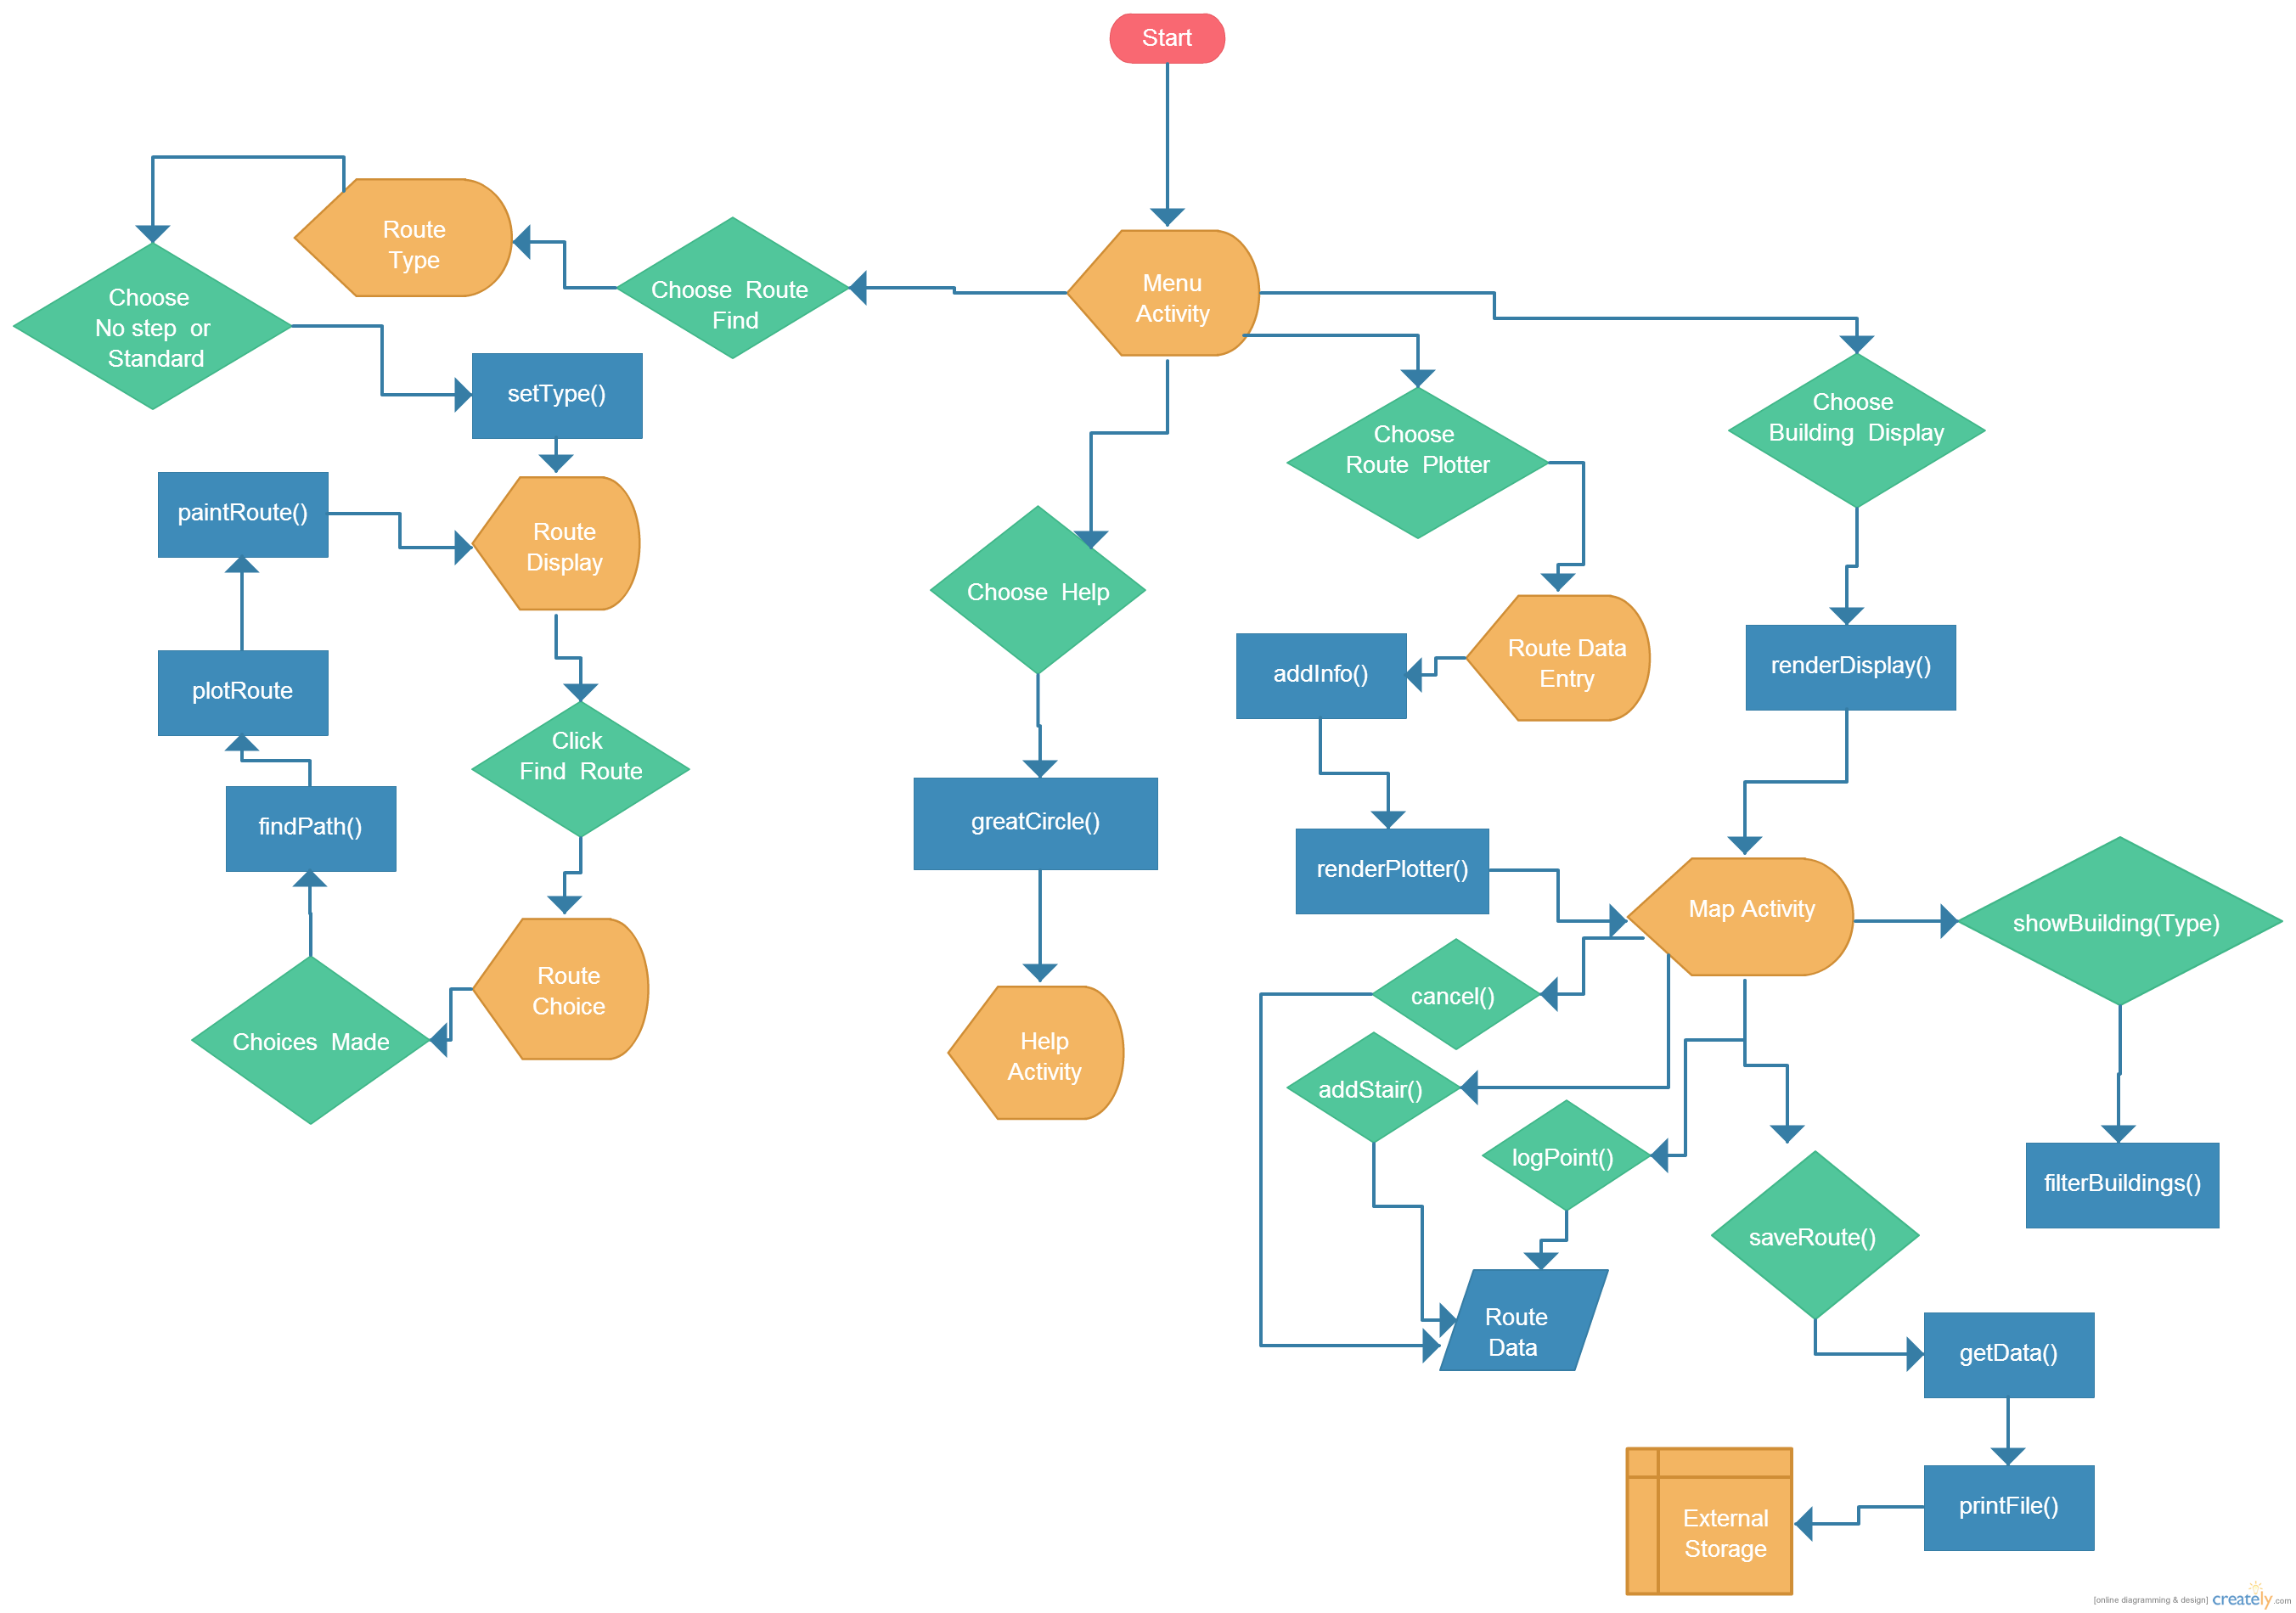
\includegraphics[scale=0.24]{Chapter2/flowo.png} \\
\end{sidewaysfigure}
\newpage
\section{Sequence Diagrams}
\section{Major Algorithms}
Throughout the application there are thought to be a range of major algorithms, most of these relate to the finding of a route and then the visualizing of that route. Currently the algorithm is expected to be a version of BFS when required to go past a single connecting node. Past designs of these algorithms can be seen in Design Specification 3.3. Following are the currently expected algorithms to find routes, calculate distance and read in the file format.

Initially route finding was shown in a single algorithm which is mostly correct, however due to the files containing all of the routes from a point the process has been changed. Initially a check will be made to see if there is a direct connection between start and end, if not then the BFS algorithms will be called. To start the algorithm should look as follows, this should check the original nodes connecting nodes. It logs the connecting nodes and if none are the destination they will be passed to the $deepFind$ which is the BFS. 

It does this by using a boolean which is changed on a route being found. At the start of the BFS it should be noted that the start node, which will be stored in the activities variables, should be added to the visited list to avoid the nodes checking that. 
\vspace{0.3cm}
\hrule
\vspace{0.1cm}
\textbf{Find Initial Path}
\vspace{0.1cm}
\hrule
\vspace{0.1cm}
\begin{algorithmic}[1]
\State$startRoutes$ = read($start$)
\State $found$ = 0
\State ArrayList $routeEnds$
\For{$startRoutes$}
	\State $routeEnds$ add $route -> end$
	\If{$route -> end = end$}
		\State Plot Single Route $route$
		\State $found$ = 1
	\EndIf
\EndFor
\If{$found == 0$}
	\State deepFind $routeEnds$
\EndIf
\end{algorithmic}

The deep find algorithm will initially be a BFS, a mostly correct version can be seen within the Design Specification however it does not account for being passed it starting nodes. The actual implementation should look close to the following pseudo code. 

In this example you can see that the start node is set to visited and the nodes to be cycled through as those passed in as a variable. While the algorithm looks relatively simple set like this due to having to implement loading from the devices memory and other functions it is expected to take time to develop. Initial research has been conducted on loading. 

A key line which helps in a later algorithm can be seen on line 11. This helps us move backwards from our destination as we can tell which connecting Node each Node was opened from, essentially plotting the path backwards by tracing the algorithms steps. 

In future it is advised that more complex search algorithms are considered, including A*, to try and find a more efficient algorithm as on a large graph BFS could cause a small delay on older mobile devices. 
\vspace{0.3cm}
\hrule
\vspace{0.1cm}
\textbf{Find Route}
\vspace{0.1cm}
\hrule
\vspace{0.1cm}
\begin{algorithmic}[1]
\State $start$ set Visited
\State $Nodes$ = $passedInNodes$
\While{!route found} this
\For{$Nodes$} 
\If {$Node$ has been visited}
    \State do nothing
\Else
	\State set $Node$ visited
    \State get $Node Routes$
    \For{$Node Routes$}
    \State Set Opened from $Node$
    	\If {$Node Route End$ = Destination}
    		\State set route found true
    		\State call Plot Path ($visited$)
    	\EndIf
    	\If {$Node Route End$ not visited}
    		\State Add to Nodes
    	\EndIf
    \EndFor
\EndIf
\EndFor
\EndWhile
\end{algorithmic}

As can be seen in the above algorithm the visited nodes are passed in as a variable to the function that will plot the path, this way access is provided to the information about which Node was opened from where, allowing the function to work backwards though the Nodes.

This is possible due to the fact that as soon as a single route is found that connects to the end no more are looked for, by doing this we guarantee only one path being painted. However this plan does not work if the search finds multiple paths, something that needs to be noted for future development. 

Due to the nested loops the algorithm should always paint all required routes. 
\vspace{0.3cm}
\hrule
\vspace{0.1cm}
\textbf{Plot Path}
\vspace{0.1cm}
\hrule
\vspace{0.1cm}
\begin{algorithmic}[1]
\State $Visited Nodes$ = $visited$
\State$search$ = destination
\For{$Visited Nodes$}
	\For{$Visited Nodes$}
	
	\If{$search = Node Name$}
		\State Plot Single Route 9$Node->name, Node->from$
		\State $search = Node from$
	\EndIf
\EndFor
\EndFor
\end{algorithmic}
Pseudo code for plotting a single route and then painting it can be found in the Design Specification sections 3.3 and 3.4. These have not changed through further design and are expected to suffice as they are. This also applies to the saving of a route file algorithm, found in section 3.5. However after research it has been noted that external memory is not always provided and as such further checks should be completed, following example code from both the Android API and other sources it is expected the following code should suffice. 
\vspace{0.3cm}
\hrule
\vspace{0.1cm}
\textbf{Plot Path}
\vspace{0.1cm}
\hrule
\vspace{0.1cm}
\begin{algorithmic}[1]
\State $state$ = $getExternalState$
\State $possWrite$ = false
\If {$state$ = $readOnly$}
	\State Cannot create files
\ElsIf{$state$ = $readWrite$}
	\State $possWrite$ = $True$
\Else{}
	\State Something is wrong, we only have one desired result which we have checked for
	\EndIf
	\State return $possWrite$

\end{algorithmic}
An algorithm which has been previously overlooked as it was initially assumed to be fairly simple is the file writer. After further research which resulted in the memory check algorithm it has been decided that its process should be noted due to the various ways it could be completed. A further decision which has been made is to include the saving of a file into the file writer function, this way when a user initially goes to save a file the folder will always be present. Initial design should be as follows. 
\vspace{0.3cm}
\hrule
\vspace{0.2cm}
\textbf{Save File}
\vspace{0.1cm}
\hrule
\vspace{0.1cm}
\begin{algorithmic}[1]
\State $root = get Memory$
\State $My Directory = root/routes$
\If{My Directory exists}
	\State Do Nothing
	\Else
\State Make Dir $->My Directory$
\EndIf
\State New File$-> root$

\State $out = Output Stream -> File$
\State $out -> Route ->Start$
\State $out -> Route -> End$
\State $out -> Route -> Grading$
\For{$Points$}
	\State $out -> Point i$
\EndFor

\end{algorithmic}
\section{Interfaces}
User Interface was an area in which the developer had little to no experience, while basic GUI's had been developed before they did not truly consider a users habits and motivations. From the initial design specification to the beginning of implementation research was completed on both good design guidelines and the options provided through Android and its use of XML for layouts. 

While UI was seen as a less important task than the actual underlying code a set of basic rules were set out from the start, taking influence from other applications and the Google Material Design outline. While the material design outline was not adhered to fully it provided good insight on the vision Google has for the Android platform. 


\begin{itemize}
	\item 1 - Make best use of white space within design, make it act as a barrier rather than having to add an actual barrier in.
	\item 2 - Bold colours will help cause distinction between background and active UI members.
	\item 3 - Theme should be carried throughout pages as best possible, little to no room for exceptions. 
	\item 4 - Develop a system which supports the same experience throughout devices. XML allows for relative layouts so no fixed measurements mostly. 
	\item 5 - Interactive elements need to be responsive, users need feedback on their actions. This can be textual or a change in colour. Noise is not practical. 
\end{itemize}
\newpage
\subsection{Colour Theme}
Colour theme was something that the developer felt was key to a successful UI, without it a good layout would go to waste. Due to this several sets of colours were chosen at the start for trial upon the full completion of the application. Intially design highlighted a yellow and purple theme as the likely choice, due to matching the universities website. However as design furthered and prototypes were developed of basic layouts, it became obvious this may not be the ideal theme. These themes were both developed internally and taken from on line resources. The following were chosen due to them being seen as palettes that would not only provide good distinction between members of the UI but provide an easy to view screen. Using many bright and clashing colours could possibly create a visually offensive UI which is something to be avoided. By using safe, strong colours a higher chance of success was predicted. 


1.

\includegraphics[scale=0.5]{Chapter2/colourone.png} \\

2.

\includegraphics[scale=0.5]{Chapter2/colourtwo.png} \\

3.
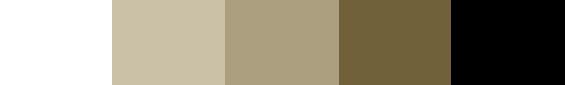
\includegraphics[scale=0.5]{Chapter2/colourthree.png} \\

As visible from the above diagram the palettes were based on what seemed to be sequential colours as such, while no actual math was applied to come to this decision it was visually apparent that the themes were a progression of shade. However this provides the developer with a range of possibilities, with the shades being far enough away from each other, text of one colour should always be visible on another due to the lack of overlap. It is advised during development though that text of one colour be on the background of a colour at least one away. 

For example, text from the middle of the first palette should only be applied to backgrounds of the two ends, while viable to put on the two connecting colours the impact of the distinct colours will be lost slightly. 


\includegraphics[scale=0.5]{Chapter2/textone.png} \\

\vspace{0.2cm}

\includegraphics[scale=0.5]{Chapter2/texttwo.png} \\
\newpage
As can be seen in the above diagrams the principle of using five progressive colour should provide us with a theme that is not only easy on the users eye but provides us with the ability to give a good distinction between UI members and blank space. With the above three options to be tested it is likely that either 1 or 2 will be the final theme. With 3 being viable the colours seem to be bland, while it could work with the right arrangement it is suggested more effort be put into a functional theme built of 1 or 2. 

A similar palette to that of 2 can be seen at outlook.com. In this design the colours are fairly similar with white acting as the background and then a colour similar to the middle acting as interactive elements. Distinction between the two can clearly be seen and as such they stand out as having a purpose, it also helps with the clear display of text while removing cluttering multiple colours may cause. In the design responsiveness is achieved through a brief colour change in the element, something that should be considered within this project. Other considerations to be made in terms of colour design is the implementation of themes for colour-blind users, however this a stretch goal and unlikely to be implemented. 

Mock up screens of the application with the prospective colour schemes can be seen below, with these it is is clear to see why 1 and 2 have an advantage over 3. It should be possible in future for the user to define a theme from a set of options, not only will this help users who make frequent use of the application but it will provide a way for the colour-blind themes to be implemented without a separate application. \\

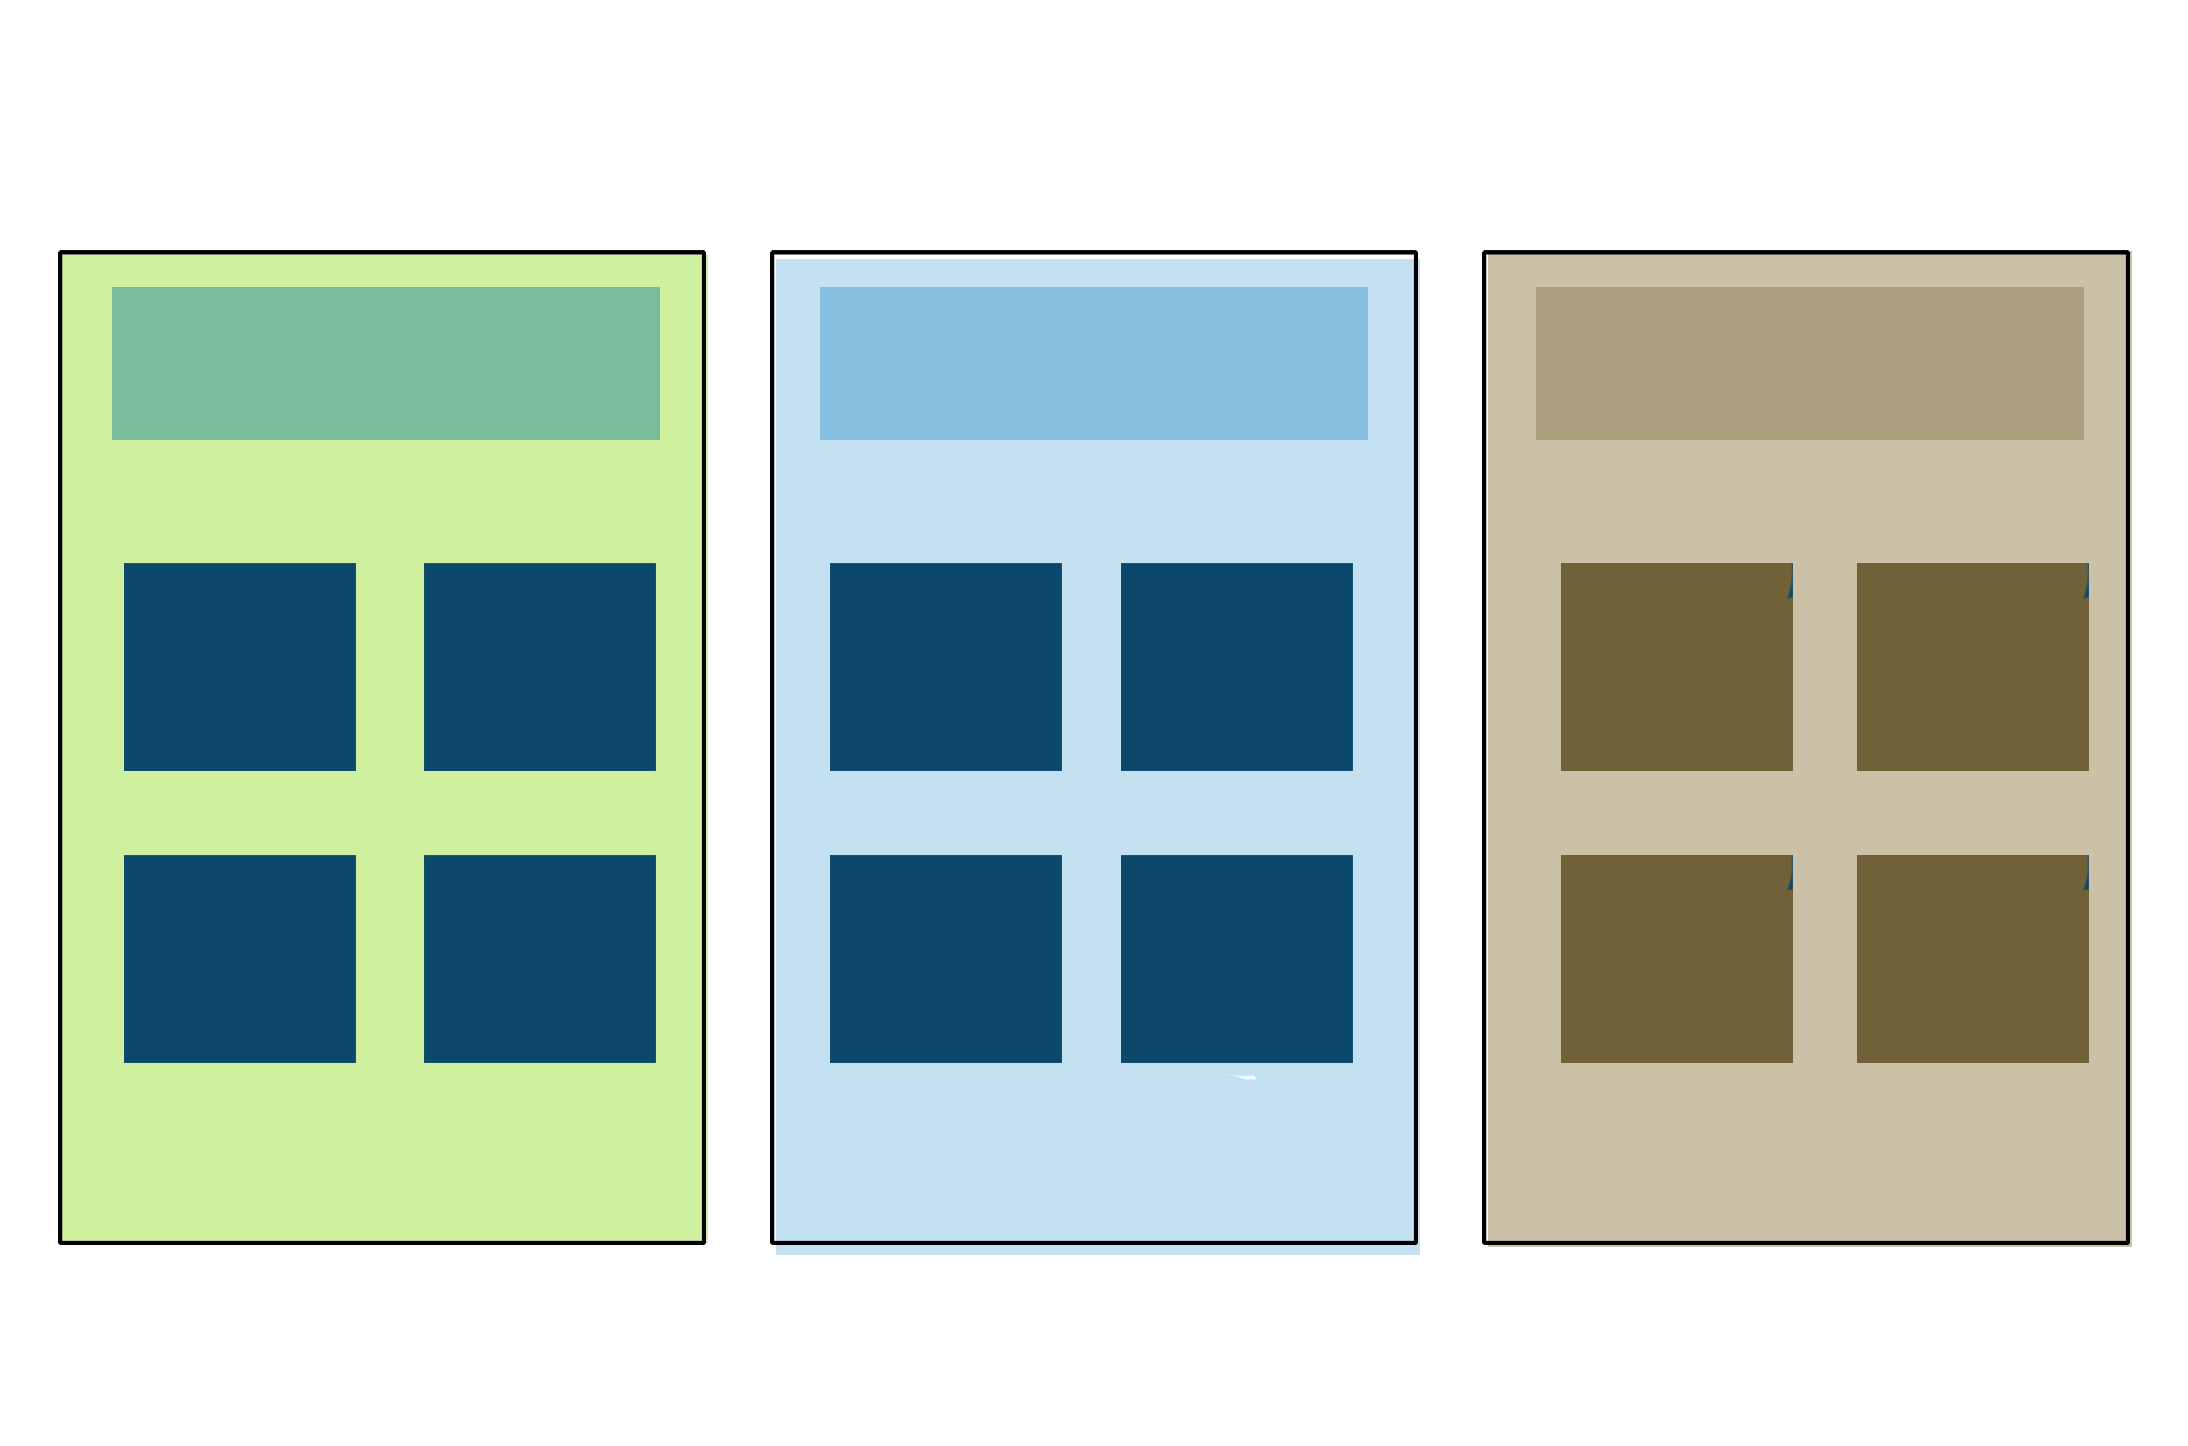
\includegraphics[scale=0.7]{Chapter2/themes.png} 
As it stands theme 1 is seen to be the most likely candidate, it provides a range of sequential yet clearly varying colours that do not look quite as unvarying as the other two options. With this visual representation it is clear to see why option 3 is unlikely, however with the use of white space it could be a viable option. Colour theme is an area that will have to be tested with the help of human users, response to a design is not something we can simulate. By completing tests on actual users not only can we plot out the decision making and adapt around it, we can get feedback on clarity, simplicity and overall operability. A fully working application that a user can easily navigate through is the prime objective of this project. 
\subsection{User location}
Display the users location to them is seen as a key element to route finding, displaying a route is only so much use if a user cannot see where they are on it. While the solution to this problem has already been discussed, some additions can be made to it. Mainly the addition of custom graphics to benefit the user. 

This is something which is covered on the introduction page to the Maps API. From that and some basic research it is possible to see that custom graphics and a movable camera are both possible. Giving the developer to implement an almost sat-nav feel to the application. 

A range of graphics have already been drawn up to discuss possible implementations of the 'arrow'.

As can be seen from the above diagram, 1 which is a representation of the basic user location does not really provide the user with too much information, it will sometimes change based on a users direction but the feedback is not obvious and those with poor vision may not be able to notice it at all. 

Possible graphic 2 is the most likely option, along with 3. These two implementations of the arrow system show the user there direction and close location without too much hindrance to view or complications based on confusing graphics. It is advised that if 2 is implemented it be made to be clearly separate from the map, while unlikely to be mistaken for a map feature a bad implementation would still allow for the possibility. Option 3 avoids this problem due to the containing circle.

Option 4 is an adapted version of 1, with the direction being clearer and as such would likely be an improvement. However with the viability of 2 and 3 being much higher it is unlikely that it will be chosen.

The theme for the guidance will follow whichever is chosen by the developer for the overall application. Creating a familiarity between the user and what they are being shown, if all interactive elements are previously shown in one colour then the arrow should follow, making it recognisable as something that will change or provide assistance. 
\subsection{Screen Designs}
Some initial screen designs can be seen in the original Design specification, while rough there overall display will not be altered too much for the development. However the theme used and some of the options made will make it hard for the screens to be implemented as they are on various screen sizes, especially on the menu screen.

In the original designs the Menu Activity is shown as a screen with a list of buttons which would then link the user to the respective Activity. However, on multiple screen sizes the buttons could start to look like they were rushed due to them just being in the middle, especially on larger screens. Due to this the decision has been made to implement a grid system on the main menu, by doing this we can make the segments relative to the screen and have them fill it. White space should also be left between the segments to provide clear non verbal instruction that the buttons are separate and interactive. 

Further changes include the addition of several screens which were not identified during the start of the project. First of these being the Route Type Activity. In this activity the user is given a choice between the two types of graph they can choose to find routes through. Following is a representation of what should be a fairly simple screen.

Another addition to the set of activities will be the Route Data Entry activity, this will allow the user to enter information about the route they are planning to take. To accomplish this the user should enter the start and end points, from there they can then move onto the actual logging of the route. Again a simple screen due to it being two text entry boxes, only restriction being that of the theme.
\newpage
\section{Other relevant sections}
\chapter{Implementation}

The implementation should look at any issues you encountered as you tried to implement your design. During the work, you might have found that elements of your design were unnecessary or overly complex; perhaps third party libraries were available that simplified some of the functions that you intended to implement. If things were easier in some areas, then how did you adapt your project to take account of your findings?

It is more likely that things were more complex than you first thought. In particular, were there any problems or difficulties that you found during implementation that you had to address? Did such problems simply delay you or were they more significant? 

You can conclude this section by reviewing the end of the implementation stage against the planned requirements.
\section{Location Based Help}
Throughout the design phase of the project the Help Activity is referred to as most likely to be the easiest feature to implement, when it came to implementation these assumptions were mostly correct.  Due to past work the developer was already aware of the Great Circle function, while research would have quickly led to the function itself it did save some time. 

There are a fair amount of changes to the implementation shown in the class diagram, some of this was done to simplify the process and stop code being used twice in two different places. The largest change is that the $calcDist$ function shown in the diagram has been pulled into its own class, this was done after initial development on the activity due to the route plotter also needing a function to calculate distance, it was best practice to only have the code exist once in the application.

Another change is the removal of the $loadHelpPoints$ function, while loading from a file is completed throughout the application in this case problems arose which made the process seem to be a waste of resources during this specific time line. While looking for information regarding people who could be contacted for help, little turned up. Details relating to three buildings were found so for the current iteration they are hard coded. 

A small change within the program is also what the $sortHelpPoints$ function returns, in the diagram it returns the sorted array. However in actuality it now returns the index of the closest location, this removes some stress on the device and is overall simpler yet still effective. A further small change is the removal of the $displayClosest$ function. In actuality this was not needed, all methods are called in the $onCreate$ due to the simple nature of the task, once the right index has been found what the method was meant to do just takes a single line of code so the inclusion of this method was seen as unnecessary.

The location based help function was actually simpler than initially thought, due to its very small size. A users location is easily found using the Location Manager and from there its basic object manipulation mostly. Implementing the great circle function took some time until a fitting one could be used, taken from Stack Overflow. Other proposed solutions seemed overly complex for what was considered, this was due to most of them including a height variable which was omitted in this case due to the small nature of campus. 

\subsection{Updating Help Location}
One idea that was experimented with was the idea of having the activity update when it moved into a new 'area' of help. This was done by repeated updating of the user location and rerunning of the methods which calculated the closest position. While it works in practice the major issue was what was seen as a good degree of uncertainty in the calculations.

While the Great Circle function works well, with its results being tested against measurements competed on Google Maps, reliability of the GPS co ordinates were not as certain. While co ordinates give us a very close estimate of our position, they are not always perfect. After some research it was clear that civilian GPS while in good conditions could return results within a metre, other factors that affect the accuracy are present on campus. Looking at figures, most GPS queries return accuracy to within 3.5 metres. However the impacting variables of receiver quality and signal blockage are not something we can plan for, due to these reasons a series of decisions were made.

As can be seen in the figure above, with the boundary between some buildings being so small, an error of 5 or so metres, something that has been seen, would provide false readings that would not be updated until the next cycle. Due to this the implemention of updating values on the Help page was omitted, the text displayed clearly displays the building the help is for, if this is wrong  a button to update values has been included.  

\section{Building Display}
During implementation a large amount of change was made to the way that the Building Display worked, a lot of this was down to it sharing an Activity with the Route Plotter. Initially this was done as the activities used similar resources and seemed small enough to not cause too many issues. However into development it was decided that the two activities really should have been separate, if nothing else than for clarities sake. However this was not decided until the features were complete, so as the project stands the screens have not been split. 
\subsection{Removal of Render functions}
In the program the largest change is the removal of the $renderPlotter$ and $renderDisplay$ functions. In past documentation these were said to be the methods that would actually render what was needed, however these have been removed and the problem handled in the $onCreate$. This is done by the press of either the Building Display Button or the Route Plotter button initially sending through a string which represents the users desire. From there the $onCreate$ is split, if the user has said they want to plot a route then a different part of the method is entered, in both cases the visibility of a set of buttons and other interactive elements is set. By doing this we can view the activity as having two $onCreate$ methods, its just that they are nested within the same parent method. 
\subsection{Other Changes}
A change seen previously is the removal of the $calcDistance$ function from this class as well, it now relies on the class that handles all of the distance algorithms. A similar change is the removal of the $loadPlaces$ function. Loading of places is handled by the actual Place class, called locations, in the application. By being moved away we keep the code in this class purely related to the displaying of locations, removing any blur between the classes. $showByType$ is implemented in the suggested way by the class diagram, it is called using the $setOnClickListener$ functions used in the $onCreate$ function. These listeners set the behaviours for an interactive element in the design, in this case the $showByType$ function is called with the buttons type being passed in as the string variable. For showing Lecture Buildings the String Lecture is passed in and the array searched for any location that matches that information. $showByType$ was actually initially implemented all in each $onClickListener$, while no real problem for the user it meant the method was implemented for however many types of building there were. When the design was finally adhered to it vastly simplified the process and created a much better class in terms of code quality. This also means that in the future any addition to the type of buildings will only need a few lines of code instead of the repeated fifteen or so which were initially being used. 

Throughout development other applications and documentation were reviewed which showed the use of custom markers for buildings, due to this the feature was also included within the application. With it only taking a small time and the result being a more customised application it was seen as a good time to improvement ratio. 

\section{Route Plotter}
Route plotting was an area in the application where a fair amount of issues arose during implementation, while the feature was successful many hard decision had to be made along the way and the result of those will have to be tested. With once again using GPS co ordinates for the positioning, problems arose with accuracy and exactly how a user would want to plot a route. Most of the class diagram relating to this feature is correct, the only difference is the movement of the log point method into the $onClickListener$.
\subsection{Plotting of points}
Plotting of points is an area which had similar issues to the updating of values in the Location Based Help feature. Mainly the testing of automatic point logging, this turned out to be a much bigger problem than in the help section. With the error in gps co ordinates sometimes being over 3 metres the automatic logging of points is not something which could be trusted to return viable results. Tests using automatic logging returned results, which when visualized, returned results similar to below. Any stop in a users movement would cause problems as any change GPS made then would cause a small difference meaning that it looked like the user was taking an erratic route.

As can be seen from the pictures above this was not an ideal way to implement the feature, what is now done is a point is only added when a user asks for it to be logged. Having the feature implemented this way means the user is free to explore paths, yet not plot them. Providing what is seen as a more user friendly experience. Another benefit found was that by using the Google Maps $locationListenerEnabled$ the user would be able to see their position, however the benefit goes further than that, in locations with good signal the point is plotted exactly at the displayed position. It is thought the reasoning is that both Google Maps and $logPoint$ method are both using a Location Manager which will always return the same results to both as its running on the same device.
\subsection{Visualizing and Cancelling}
Visualizing a route was implemented in the way detailed throughout the application, poly lines are drawn between each consecutive point causing a route which displays the users position throughout. Within the application every time a point is logged, except for the first time, the $paintRoute$ function is called, it takes the latest and previous logged point and simply paints a line between the two.

An implemented method which was not expected to be within the class is the $showDialog$ method, this is run when the user wants to cancel a walk. Absence of this method in the class diagram and other specifications is due to what was a lack of research on the possibility of a dialog box. It was wrongly assumed that the displaying of one would be smaller than it actually is, however the method is fairly simple. On the user wanting to cancel a walk, all points are wiped and the map cleared, on choosing no nothing is done. A further decision made here was whether to return the user to the data entry screen to reset the walk, however it is has been currently decided that a user cancelling a walk is more likely to be due to an error than anything else. Due to this route information is persistent unless the user chooses to go backwards to the data entry screen. 

\subsection{File Saving}
Saving the plotted route to a file was a task which took much longer than expected, this was due to a misread of the documentation. Through research it was found that an Android device typically has two types of storage, internal and external. It was assumed that external storage would only be possible with an SD card in the device, this was the first mistake which caused the long delay. A second compounding error was the assumption that saving to the internal memory would make the file accessible by the user, something which is only possible in cases where a device is rooted. These compounding factors caused the process to take a length of time which simply was not expected and set the development off by around two working days. 

During this time it was assumed that the file was simply not being created, however in actuality it was, it was just not available through any file browser, only through the application itself. This was due to the assumption that internal memory was accessible by anyone at any time, in reality files saved by applications to internal memory are only available to that application. Due to this, looking through the file system for the relevant folder was of no use, it was there but hidden. To combat this various techniques were researched of saving files without having to rely on an SD card as not all users would have them. 

One possible method was has been mentioned before was the uploading of a route so the user could retrieve it from any web connected device. Legacy code from previous projects was used to send of a JSON that included all of the relevant file information, using the LogCat feature in the Android Studio IDE showed that the data was being sent out, so the development could continue.

However, with further reference to some Stack Overflow answers to relevant questions, it was discovered that external memory is a fairly inaccurate name for what the memory actually is. In reality external memory represent one of two things, that an SD card is present or the device in question has inbuilt memory to store files. With this discovery the viablity of storing files locally vastly improved. As most devices are present with one or the other the final decision was that saving to external memory was the solution. With Google themselves trying to set the trend of removing the necessity of SD cards in Android devices it should be a smart decision for the future as well. 

\subsection{Writing to File}
Implementing this feature was simple once the problem of saving a file and accessing it were resolved. This functionality is provided by the $printFile$ method. This method takes the Route object and uses its variables to print a file that represents the route plotted. It is printed in such a way that it is compatible with the route finding side of the project. 

Printing the file is done with an $outputStreamWriter$ which takes a String and prints it into the file, each time a $write$ is called the writer uses a new line. Formatting for the file is as follows
$Start$\\
$Destination$\\
$Grading$\\
$Number of Points$\\
$Points$\\
$Destination$\\
$Grading$\\
$Number of Points$\\
$Points$\\
The format was dictated during the development of the route finder, having the file formatted as such allows for an easy implementation of a file reader. With the first 4 lines being static throughout files and the next being decided by the fourth line the code is easy to implement. From there we can see that another destination is listed, the above file contains details a Node which connects to two others and the path between them. 

Once the file is saved it is up to the user what they wish to do with it, this could range from testing of a path to full implementation to the graph. While a printed file links a Node into the graph changes still need to be made to detail the path to the Node for the user of other Nodes. This means changes need to be made to at least one other Nodes file for the Node to be fully linked. While this is not ideal there are very few ways around it, one possible way considered was to also create another file for the place the path connects to, which would contain the new path. However if multiple new paths were implemented at once, each time the new file for the Node would differ, addition by hand is not ideal but at least lets the user keep track of which files need what adding to them. 

\section{Route Plotting}
Route plotting was the key area of the application, this was due to the poor implementation of it in the original Access Aber. With so much feedback from the original version it was easy to set out a set of guidelines, some of which have been mentioned in the previous Design Specification. To begin with in the implementation a set of guidelines were set out which, if met, would cause the feature to be seen as a success for the current time line. 

\begin{itemize}
	\item 1 - Adapt the Route selector to be two selectors, a start and destination, rather than one which contains all possible routes.
	\item 2 - Implement an extendible graph that represents the campus and building locations.
	\item 3 - Have the route display gradings for the route, if the route is in segments display each segment in its respective colour.
	\item 4 - Give the user the opportunity to take a route with no steps, ideally this would be done on the same graph as standard route finding if possible.
	\item 5 - Display basic information about the route, stairs and distance ideally.  
\end{itemize}

These four criteria were seen as fairly reasonable targets, with the only worrying task being the no step feature, something which was known would be difficult. Item 5 was seen as a stretch goal as it would require the editing of the file format and as such a fairly large amount of code from some small prototypes and the route plotter.

Initial development time was used to implement the route object, something fairly simple. As an object itself the Route contains the information relating to its start, destination and the points along the route. This means it contains an Array List of what are called locations in the application, labelled places on the class diagram. This implementation, though simple, provides us with all of the information needed to find a path through the graph. When a Node is analysed, what is really happening is that a file is being loaded in which creates a set of routes, each are checked for where they end. If the route ends at the right place the solution is found, if not its end place is added as a Node to be searched next. 

Paths between nodes are stored as a set of locations, this is an object used repeatedly throughout the application, a 'locations' object contains a range of information, most importantly the co ordinates of the point. For route finding the rest of the information possible is irrelevant, other variables are used elsewhere. Having this one object which describes a location was a real benefit during development, it saved creating classes for what were meant to be different types of location like buildings. Due to this locations can have names and descriptions, it is just that they are not important for route finding. 

\chapter{Testing}

\section{Overall Approach to Testing}
Overall approach to testing was fairly simple, with the completion of each feature any relevant tests were either coded or completed by the developer. This included unit testing, stress testing and acceptance testing. Due to the applications aim of helping a user it was important the UI was received well. 
\subsection{Problems Encountered}
Throughout testing many issues arose, many more than were found in development. Getting a working test environment functional for the first time was much more complicated than expected, with references to this around the web it is not an isolated incident. Problems included - 
\begin{itemize}
  \item Out of date documentation on the official Google Developer site.
  \item Bugs in the current (1.2) version of Android Studio which will show an empty test suite despite the tests being there, ran and results printed.
  \item Lack of official support for unit testing in Activity classes, while it seems possible the issues it proves are numerous. Alternatives were discovered near the end of the project time line but a lack of time meant other more important tasks were completed.  
\end{itemize}

In future projects more time will have to be dedicated to the testing of the application. It is thought the issues encountered with testing were down to mix of issues, mainly the early stages of Android Studios official release and the tight schedule for testing including final acceptance testing. 
\section{Automated Testing}
Automated testing was completed throughout the duration of the project, problems with unit testing were previously discussed however Android did have other important utilities to make use of which helped with thorough testing, especially looking for crash cases.
\subsection{Unit Tests}
Despite the issues encountered, unit testing was completed on the non Activity classes. This included the testing of correct behaviour from the classes to handle distance calculations and from the Objects which made up a Route Object. While the tests results would not appear within the IDE due to a known bug it was still possible to see the results in a created HTML document logging pass percentage. While it would have been beneficial to complete more Unit testing it would have required the re structuring of the program and reversal of many design decisions. While an attempt to follow a MVP pattern was made, as can be seen with the XML, Route Display Activity and Route object, in future it is advised it is stuck to more thoroughly to aid with testing. 

\begin{figure}[H]
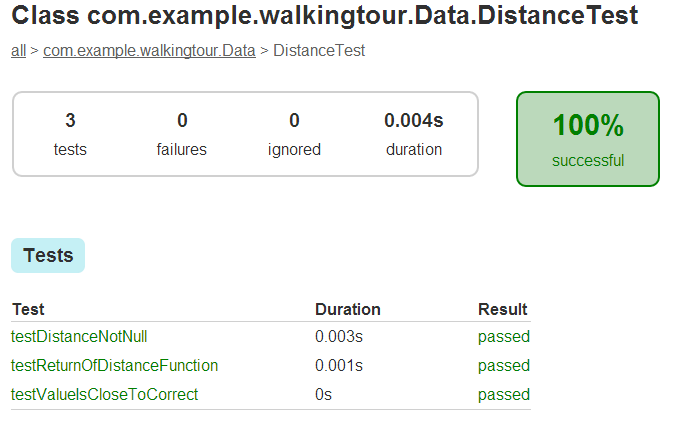
\includegraphics[scale=0.5]{Chapter4/unit.png} 
\caption[Test Output]{Image displaying the output from running a set of tests, these are results from a single small set of tests.}
\end{figure}
\subsection{Stress Testing}
Stress testing was completed with the use of 'The Monkey'. 'The Monkey' is a tool which sends a range of inputs to the application and logs the results of this at the end of its run. By doing this the application is spammed with events and any area of the application where hang ups in performance can cause crashes should be found. Through final stress testing well over 200,000 inputs have been simulated and no serious faults can be found in the application in this way. However this does not mean that faults are not there, just hard to find if they are. 

Throughout stress testing one issue which has been prevalent however has been the lack of support for the cancelling of activities, this has been noted in both the route data entry screen and the route choice screen. Since then these have been handled along with the addition of further tests in the code to deal with a user selecting the same location as a start and destination. 

Using 'The Monkey' tool was a real benefit for the developer, as pointed out while it found no significant errors the ones it did find would have caused a real effect on the usability of the application. In future it is advised any improvement to the application be tested in such a way, the tool can be limited to the use of a single package and as such can be fine tuned to send demands to the right class. 

\begin{figure}[H]
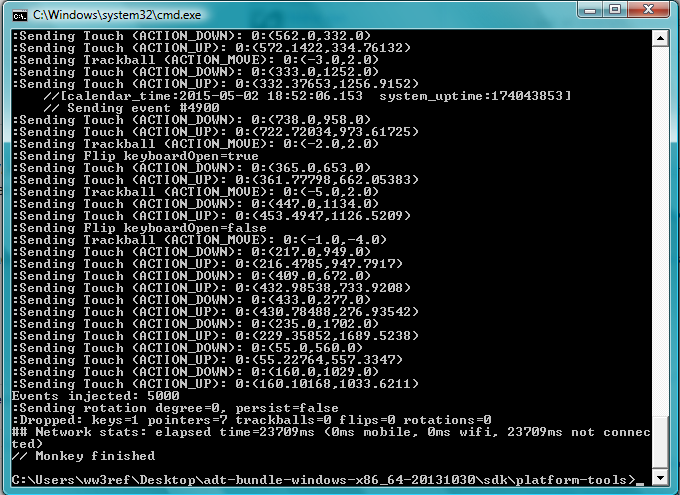
\includegraphics[scale=0.5]{Chapter4/monkey.png} 
\caption[Monkey Stress Test]{Image displaying the results of a Monkey run using 5000 inputs resulting in no dropped actions and no crashes on the device side.}
\end{figure}

\section{Integration Testing}
While some integration testing was completed there is little to document due to the nature of the application. This is down to the fact that the functionality within the application are essentially singular branches accessed through the Menu Activity. As this is the structure, very little is passed between multiple functionalities, the only place this can be seen is the file from the Route Plotter being compatible with the Route Finder graph structure. So while testing was completed, the initial unit testing combined with final acceptance testing was seen as sufficient.
\section{User Testing}
After initial development a small user group was used to determine some UI elements, this mainly related to the use of the application for first time users and the overall visual appeal of the application. For these tests users were asked to perform a variety of tasks relating to the functional requirements, the results of these can be seen in the Appendix section. Users were also asked for their opinion on the colour scheme of the application, this was done through the use of different themes for different pages on the test application. While some of the features were a little bare at the time they were all fully functional, just not polished. 
\section{Acceptance Testing}
Acceptance Testing was performed by the developer of the application, a list of tests was drawn up to determine the full functionality of the application including cases which may cause crashes from poor quality code. The test tables which represent this information can be found in Appendix section x. Some were completed after full development, others during development.
\chapter{Evaluation}

Examiners expect to find in your dissertation a section addressing such questions as:

\begin{itemize}
   \item Were the requirements correctly identified? 
   \item Were the design decisions correct?
   \item Could a more suitable set of tools have been chosen?
   \item How well did the software meet the needs of those who were expecting to use it?
   \item How well were any other project aims achieved?
   \item If you were starting again, what would you do differently?
\end{itemize}

Such material is regarded as an important part of the dissertation; it should demonstrate that you are capable not only of carrying out a piece of work but also of thinking critically about how you did it and how you might have done it better. This is seen as an important part of an honours degree. 

There will be good things and room for improvement with any project. As you write this section, identify and discuss the parts of the work that went well and also consider ways in which the work could be improved. 

Review the discussion on the Evaluation section from the lectures. A recording is available on Blackboard. 
% add any additional chapters here

\setemptyheader
\addcontentsline{toc}{chapter}{Appendices}
\chapter*{Appendices}
\pagebreak

% start the appendix - sets up different numbering
\fancypagestyle{plain}{%
%\fancyhf{} % clear all header and footer fields
\fancyhead[L]{\textsl{Appendix\ \thechapter}}
\fancyhead[R]{\textsl{\leftmark}}}

\appendix
\fancyhead[L]{\textsl{Appendix\ \thechapter}}
\fancyhead[R]{\textsl{\leftmark}}
\fancyhead[C]{}
\fancyfoot[C]{\thepage}
\renewcommand{\headrulewidth}{0.4pt}
\renewcommand{\chaptermark}[1]{\markboth{#1}{}}

\fancyhead[L]{\textsl{Appendix\ \thechapter}}
\fancyhead[R]{\textsl{\leftmark}}
\fancyfoot[C]{{\thepage} of \pageref{LastPage}}

% include any appendices here

\chapter{Third-Party Code and Libraries}
A small amount of third part code was used throughout the project.

Greater circle function.\cite{circlef}
\begin{lstlisting}
private double distance(double lat1, double lat2, double lon1, double lon2,
        double el1, double el2) {

    final int R = 6371; // Radius of the earth

    Double latDistance = deg2rad(lat2 - lat1);
    Double lonDistance = deg2rad(lon2 - lon1);
    Double a = Math.sin(latDistance / 2) * Math.sin(latDistance / 2)
            + Math.cos(deg2rad(lat1)) * Math.cos(deg2rad(lat2))
            * Math.sin(lonDistance / 2) * Math.sin(lonDistance / 2);
    Double c = 2 * Math.atan2(Math.sqrt(a), Math.sqrt(1 - a));
    double distance = R * c * 1000; // convert to meters

    double height = el1 - el2;
    distance = Math.pow(distance, 2) + Math.pow(height, 2);
    return Math.sqrt(distance);
}

private double deg2rad(double deg) {
    return (deg * Math.PI / 180.0);
}
\end{lstlisting}
\newpage
Custom Button development.\cite{button}
\begin{lstlisting}
<?xml version="1.0" encoding="utf-8"?>
<selector xmlns:android="http://schemas.android.com/apk/res/android" >
     <item android:state_pressed="true" >
         <shape android:shape="rectangle"  >
             <corners android:radius="3dip" />
             <stroke android:width="1dip" android:color="#83776b" />
             <gradient  android:angle="-90"  android:startColor="#5f4427"
              android:endColor="#cbb59d"  />            
         </shape>
     </item>
    <item android:state_focused="true">
         <shape android:shape="rectangle"  >
             <corners android:radius="3dip" />
             <stroke android:width="1dip" android:color="#83776b" />
             <solid  android:color="#92806c"/>       
         </shape>
     </item>  
    <item >
        <shape android:shape="rectangle"  >
             <corners android:radius="3dip" />
             <stroke android:width="1dip" android:color="#83776b" />
             <gradient  android:angle="-90"  android:startColor="#cbb59d" 
             android:endColor="#92806c" />            
         </shape>
     </item>
</selector>$

$<style name="btnStyleSandrift" parent="@android:style/Widget.Button">
       <item name="android:textSize">15sp</item>
       <item name="android:textStyle">bold</item>
       <item name="android:textColor">#FFFFFF</item>
       <item name="android:gravity">center</item>
       <item name="android:shadowColor">#000000</item>
       <item name="android:shadowDx">1</item>
       <item name="android:shadowDy">1</item>
       <item name="android:shadowRadius">0.6</item>
       <item name="android:background">@drawable/custom_btn_sandrift</item>
       <item name="android:padding">10dip</item>
   </style>$
   
\end{lstlisting}
\chapter{Code samples}
\section{Random Number Generator}

The Bayes Durham Shuffle ensures that the psuedo random numbers used in the simulation are further shuffled, ensuring minimal correlation between subsequent random outputs \cite{NumericalRecipes}.

\begin{verbatim}
 #define IM1 2147483563
 #define IM2 2147483399
 #define AM (1.0/IM1)
 #define IMM1 (IM1-1)
 #define IA1 40014
 #define IA2 40692 
 #define IQ1 53668
 #define IQ2 52774
 #define IR1 12211
 #define IR2 3791
 #define NTAB 32
 #define NDIV (1+IMM1/NTAB)
 #define EPS 1.2e-7
 #define RNMX (1.0 - EPS)
 
 double ran2(long *idum)
 {
   /*---------------------------------------------------*/
   /* Minimum Standard Random Number Generator          */
   /* Taken from Numerical recipies in C                */
   /* Based on Park and Miller with Bays Durham Shuffle */
   /* Coupled Schrage methods for extra periodicity     */
   /* Always call with negative number to initialise    */
   /*---------------------------------------------------*/	
 
   int j;
   long k;
   static long idum2=123456789;
   static long iy=0;
   static long iv[NTAB];
   double temp;
 
   if (*idum <=0)
   {
     if (-(*idum) < 1)
     {
       *idum = 1;
     }else
     {
       *idum = -(*idum);
     }
     idum2=(*idum);
     for (j=NTAB+7;j>=0;j--)
     {
       k = (*idum)/IQ1;
       *idum = IA1 *(*idum-k*IQ1) - IR1*k;
       if (*idum < 0)
       {
         *idum += IM1;
       }
       if (j < NTAB)
       {
         iv[j] = *idum;
       }
     }
     iy = iv[0];	
   }
   k = (*idum)/IQ1;
   *idum = IA1*(*idum-k*IQ1) - IR1*k;
   if (*idum < 0)
   {
     *idum += IM1;
   }
   k = (idum2)/IQ2;
   idum2 = IA2*(idum2-k*IQ2) - IR2*k;
   if (idum2 < 0)
   {
     idum2 += IM2;
   }
   j = iy/NDIV;
   iy=iv[j] - idum2;
   iv[j] = *idum;
   if (iy < 1)
   {
     iy += IMM1;
   }
   if ((temp=AM*iy) > RNMX)
   {
     return RNMX;
   }else
   {
     return temp;	
   }
 }
 
\end{verbatim}


\chapter{Requirements Specification}


\section{Functionality}

The major aim for this project is to provide an android alternative to the already existing Access Aber web application. Currently the project exists solely as a web application which can be run on both iOS and Android through the use of a web browser. However the project is limited due to the time it was developed in and it is my aim to show that developing the application native to one environment can provide benefits which make the time and effort worth it. The idea is to not only port over the existing application but to improve upon it in ways that are seen fit. I feel that with the power given to a programmer within not just android, but mobile devices in general, the application can be made to be not only effective but intuitive and an asset to those who visit campus. The application will consist of several areas that will benefit the user and will heavily rely on the Google Maps Android API. 
\subsection{Route Finding}
One of the main features to be included is that of a route finding system around campus. This differs from the web application due to the system actually finding a route, as it stands the application has around 200 stored routes which a user can select from. However these are displayed as a list and require the user to spend a large time searching through with no guarantee of there route actually being stored.

The android application will be developed in a different way. The user must be able to find there way around campus without having to search through 200 routes. The plan to combat this is to first have a much simpler way of route selection, ideally this will be two drop down boxes where a user selects where they are and where they want to go. This means that if we cover 20 locations, we just need 20 options instead of representing it as over 400 hard coded routes which is what would be needed in the current set up. 

The second plan to combat the current issue is to remove most hard coded routes. All that ideally has to be implemented is for each building to connect to at least one other. If this is implemented correctly we can instead search for a Route rather than store them. This saves the user time and means that the application should be easily extendible. 

One issue which arose in a meeting with the section of the University which initially set up the project was that while routes were shown not much else was. No information regarding the route and no indication of the difficulty of it, both of these would be of a lot of use especially to disabled users of the application. It is already known that colour coded routes should be possible within the application, combining this with a small window which shows information such as distance,elevation and steps on the route should fix this problem which has been highlighted. 
\subsection{Route Plotting}
Another issue that arose within the meetings was that the plotting of a route was done manually, the only visualization the user inputting it had is whatever setting was provided through Google Maps. It was suggested that a suitable addition would be a route plotter which let the user walk a route and logged it for them. 

Due to the planned nature of the system all that will hopefully be required is for the user to plot one route that connects to the graph of locations. By following this process we can fulfil another requirement that was brought up within discussions, the adding of information about a route. It may be possible to build a step free graph, thus allowing guaranteed step free routes. Some buildings are inaccessible so they would have to be omitted from this feature. 
\subsection{Location Based Help}
A further requirement is the fulfilment of a help service for those on campus. Aberystwyth's campus can be a hard place to traverse along with confusing if it is your first time visiting. Due to this it is very possible that a user will require help to either exit a building or enter another, while help will be provided through another feature mapping the indoors of buildings will not be included in the application due to time constraints. To combat this a help service will need to be included, this will display to the user the closest person who may be able to provide some assistance to them.

Not only will this help the user if its needed, the presence of it should assure them even if it is not required. It has been noted previously that even some members of staff with mobility issues do not enter some buildings due to them being poorly labelled and other factors. This may be somewhat of a help to a complex situation.
\subsection{Building Display}
This is a feature that will be brought straight over from the existing application with only a few changes. It will provide a list of categories and let the user choose which they would like to view and then provide a display of where they are. 

The feedback from the initial application is something which will be of great use here. There were several possible additions including pictures instead of just markers, something which is very possible and the inclusion of building names above names of lecture theatres as it can be unclear exactly where something is due to departments sharing buildings. 
\subsection{Multi Lingual Support}
Due to this being a Welsh University it is required that welsh language support is provided for the likely event that a native welsh speaker uses the application.

This is an area which can pose problems. Android appears to have little to no support for the inclusion of Welsh language however new locales can be created and used which should help solve the problem. 

\section{Interfaces}
\subsection{User Interface}
\subsubsection{General User}
The General User must have access to all features except the route plotter. The route plotter gives them no added actual use for their specific needs, however it is currently undecided if the project will be split up into two separate projects or just built as one and adapted from there. Having the Route plotter within the main application may confuse the user to a degree as unless you are aware of what its doing it will not appear to provide much of a benefit. It is likely it will be left in unless further use can be seen in splitting it up from the main part of the development.

Future development could focus on providing different User Interface based on the user type. This could be focused down further to provide different functionality based on a users mobility level. However in the time scale provided it is unlikely that this feature will be done now, if anything some level of customisation may be provided relating to route finding but not much else.
\subsubsection{Staff Users}
Staff users need access to all features, for addition to the system and to check everything is up to date. This is not a problem.
\subsubsection{Encountered User Criticisms}
Using the already completed user feedback results for the web application we can already start to set out some rough requirements for the look of the application and what needs to be shown. One major criticism was the fact that users are dropped straight into the map, this means that from there you have to work out what does what within the application. This also links to the problem of the buttons used currently being small and non intuitive which causes issues in itself.

This means its become a requirement to fix these base problems, most other problems highlighted link back to the confusing nature of the current User Interface. A huge improvement needs to be made to this, while some elements like the colour scheme are suitable for the purpose overall it is clear why users have issue with it. A possible solution is having a menu of sorts that is clearly labelled which then launches separate features meaning a simpler UI on each screen and no cluttering or extensive menus. 

Other criticisms which effected user experience were related somewhat to the labelling of information within the site. It was not always clear if a labelled room was correct due to it appearing around other rooms for other departments. This is due to departments sharing buildings and is a fairly simple fix as all that needs to be done is to label each room with its respective information. 
\subsection{Google Services}
The application will have to interface with several of Google's services. This mainly relates to interfacing with the map service which requires an API key, in this case API keys are free and will give us more than enough requests a day to develop the application. Using the Google Map service gives us a large range of benefits due to their thorough API, this allows for the development of elements like visualising a route on screen, showing a user there progress and markers for displaying building locations. 

Having this thorough API is key to the success of the project, other possibilities have been explored including Open Street Maps but due to the developers past experience and what are seen to be gaps within the OSM API the Google Service has been chosen. While the service lacks some of the detail that may be seen as useful the benefits it gives more than make up for it and means that we can cover any gaps with our own implementations. The ability to customise elements of the maps is also a welcome addition and should help with the development of the labelling of buildings and displaying route paths and their grading. 
\subsection{Hardware}
The application will also have to interface with hardware elements within the mobile devices. This mainly means the GPS module and possibly sensors to detect the gradient of a slope. Interfacing with the GPS module is made easy through the use of the Location Manager available through Android, this provides us with a periodic update of the users position allowing us to plot routes, display their position to them and to make estimations on who is best to contact for help.

It is also possible that the Camera will be used to help with plotting routes however it is more of a suggestion than a requirement. If this is implemented it means a picture would be displayed of both the start of the route and the end destination. Doing this will mean that the user has a visual aid to help with finding their building as there could be some error with very close together destinations. 
\subsection{Interfacing with itself.}
The application will also have to interface with itself in a way, the files created by the route plotter need to be ready to just add into the projects resources and work straight away. While this is less of a straight one to one interface the elements of the application need to be compatibly with each other, maybe an obvious requirement but necessary. 

\section{Performance}
\subsection{Offline Performance}
There are several areas within the application where performance can be effected by what is to be completed. One major issue with this is that the application simply cannot work with no Internet Connection, at least not the first time round. The application has to load in the Google Map object and to do that and have the relevant imagery a connection is required. In this case the only real requirement is to at least notify a user of this and notify them if their is no current connection. A blank screen is shown by default when there is a lack of connection which needs to be remedied. It is suggested that a tech spike into caching imagery of the surrounding area is completed to make the application fully functional even when offline. 
\subsection{Searching Algorithm}
A further area which could provide small problems, especially on older phones, is the searching for a route. However it is unlikely with the expected size of the graph that the algorithm created will cause too much effect. It is hard to set a requirement regarding the search, we need to it perform well but without an existing set up it is hard to test what we feel is a good range. However for the current stage of the project it is sufficient to say we need to test on a range of devices to find a good middle ground. 
\subsection{Possible Problem areas.}
In addition to the performance issues previously we also need to ensure the performance of the GPS module, it is very possible that errors are made using cached values for the latitude and longitude but this should be a fairly easy fix. By guaranteeing new readings we improve our accuracy and provide the user with the route they actually plotted. 

Performance wise we also have to take into account the responsiveness of the application. It is a common problem to encounter freezing and unclear interfaces within applications. To combat this steps need to be taken to not only improve code quality but provide a view that keeps the user updated on what is happening. Its not too much of a problem if it takes two seconds for a route to be found if the user is at least told about what function is being carried out. 

One last problem area involves the performance on a range of screen sizes, the UI has to be coded in such a way that it does not depend on fixed sizes and instead relative ones. By doing this we ensure a consistent and appealing design despite device. 

\section{Attributes}
\subsection{Maintainability}
A big issue with the application will be the maintainability of it; there is no guarantee the initial developer will always be around to change or fix it and as such this provides some restrictions on development. It means a high level of code quality needs to be maintained, while this is ideal in all projects it is maybe more so in this project as the chances of it being passed on could be quite high. This means full documentation, concise and clear comments and possibly JavaDoc but this will be decided at a later date. 

Maintaining up to date information regarding locations of buildings and facilities is also something that needs to be considered. The issue here is whether we want to trust that a user can access the internet and gather the needed information from there or if it should come on device. Keeping the information on device means that an update is needed to change any of the information. Maybe not an ideal solution but possibly the best. 
\subsection{Expandability}
This is a section with a large amount of requirements, the solutions to which will be fully considered in the design documentation due to the in depth analysis needed. The first problem is that its very possible the application will need expanding in future, because of this we need to make it as simple as possible to expand it for users that might not have large technical experience. 

Due to this the code will have to read in information, and analyse it, using no built in constants. It needs to be developed in such a way that the files that contain the information guide the software as such. By doing this we keep a solid sensible structure to the information which will be easy to pull out with file reading algorithms in the code itself. The problem with this is that an error in a file could cause huge problems, however error checking in the file reader should help us solve that problem in somewhat of a sensible way. 
\subsubsection{Expanding the Graph}

The big issue with expandability is the ability to add new locations to the route finder and as such expand the graph. It is possible that users with low technical expertise could be the ones responsible for expanding the project in future and as such the initial development has to make it easy for changes in the future.

To do this it is suggested that a simple set of instructions is clearly written up which describes in detail the process of adding in a new location. Ideally this will just mean creating a new file that contains the information of a locations name and a route into the graph of nodes. By implementing it in this way the maintainer does not have to understand the workings of the search or the traversal of a graph, just how to write out a basic file. A location file should ideally contain the start name, then details about its connecting nodes and the latitude longitude points which make up the link between the nodes.

It is essential that no code has to be changed to include these additions, relying on fixed variables in the code will cause large issues further down the time line of the project, beyond the initial building. 
\subsubsection{Expanding Choices}
A further issue which arises with expandability is with the adding of new locations and how we can make it so they are recognised and added to existing menus in the application. This mainly effects the selecting of the start and destination in route finding, the current plan is to load all possible places from a single file so adding to the menu would simply mean attaching a location to the end of a word file, something most people are capable of. 

By having adaptive menu choices we keep further developers away from old code that may not be as intuitive as it might need to be. Having the application set up so that it can be expanded without the editing of existing code will be a real bonus as was described in the initial meetings. 

\subsection{Security}
Security issues are something we do not really need to consider given the nature of the application. The user does not provide us with any personal information and there is no sensitive information included within the application. All data used will be publicly available and the code open sourced. 

One way in which this might change in the future is the inclusion of directly uploading routes to the application and having devices load them from there. If this is developed in the future it is advised that great care is taken due to the damage that can be done through the inclusion of fake locations and misleading information. 

\subsection{Design}
Design is an attribute that will need further research, this is due to Google releasing design guidelines to improve the quality of android applications due to an increasing opinion of iOS applications looking much cleaner and professional. However one consideration is access for those with vision impairment.

During the project time line and definitely in any further development a consideration to take is assistance to those with impairment. This can come in the way of multiple colour themes to help those with types of colour blindness as well as a possible sort of Sat Nav feature.

This feature would read out directions for the user, not only benefiting those with vision impairment but any general user. Maps can sometimes be a little unclear so if we provide instructions for when a user is at a specific GPS co ordinate then we know we are giving them enough information to properly follow the route provided. 
\subsubsection{Route Design}
The design of the route displayed is also an important element with a range of requirements. First of all as previously described the user needs to be able to see the difficulty of the route. With the plan being displaying large routes made up of much smaller ones we will be able to display the difficulty of smaller sections than the whole path. This means users can see where the difficulty may lie and possibly find a way around it. With campus being fairly condensed with winding paths and roads its sometimes difficult to tell what is coming up. For disabled users to know that a path further on has a high incline could be valuable information. 

To build on route design it is also required that the display is intuitive. This should be helped by the facilities provided by the Google Maps API. Being able to show a users location and orientation will be very useful especially if a custom arrow graphic is used rather than the standard dot. It is also important that the start and end points be clearly labelled to help with orientation. 
\newpage
\subsection{Overall User Interface}
The application must follow a consistent and appealing graphical interface throughout. This will help build up the users familiarity and help improve the intuitiveness of the design. This includes several guidelines which will be laid out in more detail in the design document but include -\\ 
	-Options are selected from Expandable List View\\
	-Pop up menus used for small actions on map screens.\\
	-Custom Button XML to provide a theme appropriate     display.
\section{Design Constraints}
The design constraints for the project are fairly obvious. The project must be android compatible and will be developed in the Android Studio IDE. It will be tested using both unit tests and black box testing with users who have no experience with the application. 

It must be compatible with the lowest Android API level possible however what that currently is will not be clear until further on into development. The current aim is no higher than API level 14 which should be possible with the current estimated feature list.

\section{Final Comment}
The project will be developed as closely to this requirement specification as possible but may deviate due to the nature or software development, while this document details what is thought to be the current best practice it is possible that the final project deviates slightly from it. 

\chapter{Design Specification}
\tableofcontents
\newpage
\section{Introduction}
\subsection{Purpose of Document}
The purpose of this document is to set out an initial design for the project 'Adapting Access Aber to android making use of native features'. It will encompass various design decisions and estimations of what the final system should look like on a code level. The final Design may differ but should lie around the boundaries set out here.
\subsection{Scope}
This Design Specification will split up the application into several components and describe any interaction within the application. Some components may essentially be stand alone except for the link to them however. This document may reference the requirements specification previously set out, it will likely reference the required functionality set out within the 'Functionality' section. For ease of use the following are the main areas of functionality required, these will be referenced by their key displayed here throughout the document. More details on each functional requirement can be found in the requirements specification.

\begin{itemize}
	\item FR1 - Route Finding - Guiding a User around campus
	\item FR2 - Route Plotting - Users must be able to plot their own routes.
	\item FR3 - Location Based Help - Provide details of possible help available.
	\item FR4 - Building Display - A display of related buildings
	\item FR5 - Multi Lingual Support - Welsh translation
\end{itemize}
 

\subsection{Objectives}
The objectives of this document are to - 
\begin{enumerate}
\item Describe the main components of the Access Aber Application (AA)\cite{aa}
\item Provide Details of interactions performed by the Application
\item To provide details about likely class interfaces
\item To provide diagrams of significant data structures and details of significant algorithms 
\end{enumerate}
\newpage
\section{Decomposition Description}
The decomposition description will provide details on the division of the modules which make up the application. It describes the structure of the system and the function of each significant module. This should give a good overview of the expected design in an abstract way. 
\subsection{Modules within the Application}
This section will describe how we expect the application to be split up for development. Due to the singular nature of most of the application, it is likely development will take place by feature rather than as a whole.

The application itself is expected to be split into 4 main modules which will be accessed through a central menu. 
\begin{enumerate}
\item A route finder for users to enter a start and destination and have a route displayed to them.
\item A help service which provides details on the closest possible person who may be able to provide help.
\item A display of buildings that the user can filter.
\item A Route plotter to help the maintainers plot routes while seeing them and the current route they're plotting. 
\item It is also possible a separate application will be developed to test the loading of route files created by the application.
\end{enumerate}
The following section will detail further design elements related to the expected modules.
\subsubsection{Route Finder}
The route finder is where the main source of issues is expected to come from, the representation of data and searching of that data is expected to pose problems and take a fair amount of time to perfect. However some steps have been taken already to research possible ways to solve this task. A searchable graph is required to avoid the issue seen in the initial web application of having too many saved routes. 

It is expected that a Breadth First Search (BFS)\cite{bfs} will be used, this is due to the guarantees it can provide us and past experience. Using BFS should mean we will provide the shortest path in terms of locations traversed, while this may not guarantee the definitive shortest path the layout of campus and the graph that is expected to be used means the least locations should always mean the least distance. While BFS can sometimes be heavy on memory use due to it storing every node on a specific 'level' it is not expected that the graph used will be overly large so issues relating to this should be mostly avoided. This also helps us combat the time issue. In a larger environment we would have significant problems and if this application is adapted in future this search may need to be swapped out for another.

Each Node will essentially be a traversable location, whether the location is a destination or not is another matter. With initial research it is obvious that the graph will have to abide by the road and walkway system within the Universities campus, so some locations may be junctions in walkways. Due to this each link between each Node should be represented as a set of Co Ordinates which we can then plot on the map provide through Google Play Services. 

It has already been decided that in an ideal solution no location will be hard coded and instead loaded in from files who follow a set format and as such can be made with the Route Plotting application to meet FR2. The source of these files is expected to be within the applications own assets, however research will be done on fetching the files from a server to see if it provides any significant benefits. Files retrieved from the internet would mean we did not need to push an update every time something changed, however it is unlikely campus will change significantly and updates should not be too common. Thus meaning local files is probably an acceptable solution especially considering the issues posed by poor signal on campus for mobile devices. 

Routes will also have a grading with them, something requested in meetings with the initial 'customers'. A Green, Amber, Red solution should be implemented letting users know the difficulty of the route they are about to follow. Due to the plan to have smaller routes make up larger ones it will be possible to highlight small segments of the route which may provide difficulty. A set of overall information should also be provided, with a user being able to see how many steps they have to take, distance and possibly elevation figured using the Google elevation API\cite{ele}. 

A further possible feature is the inclusion of a step free graph, this will be exactly like the current graph but a version that includes no steps on the way. By doing this we make the application more accessible. It should be fairly routine to expand to this idea, all that should be required is a new set of files for locations and their links. 
\subsubsection{Route Plotting}
Route plotting should be a fairly simple implementation but still fill the needs of the User. Route plotting will take place using a Google Map object and the Location Manager provided within the Android API\cite{api}. A user will be able to click a button and the onClick() Event will call a refresh on the users position. By doing this we should be able to provide accurate co ordinates. Each time a user has clicked a Poly Line object will also be added to the map detailing the current route shown. By doing this the user has a visual representation of what is happening. Poly Lines will also be used for showing routes on the route finder. It should also be possible to add information relating to inclines and steps if possible within the time scale of the project. 

The Route Plotter will provide functionality to cancel the current route or write it to a application compatible file. The file will fit the format expected from the reader, by doing this we guarantee a working way to create new files, it stops errors occurring on the human end of expanding the application. 

It is possible to remove this module and make it its own application but the benefits of this seem insignificant. Due to this it is most likely this module will be accessible through the main menu, clearly labelled. This way we hope to avoid confusion, no negative actions can be instantiated through the route plotter due to the files saving to the device. While possible to upload to a site, the added work created by doing this for a small part of the application makes it difficult for the development time to be worth it.

Route plotting should also include the generating of a grading for the route, again taking into account  total distance, steps included and elevation. By doing this we create a general idea for the user about what is on the route they've been given. Routes with no steps should be at a maximum graded amber for ease of use, the defining factor between a route being green and amber will be based on total distance and elevation difference in comparison to the distance. 

\subsubsection{Location Based Help}
The application should also provide the user with information about receiving help. However it is possible to take this one step further and suggest help based on location. By doing this we minimize the possibility of someone requesting help from a person who cannot provide it from where they are. It should also make users feel more comfortable by knowing that help is available, this was something else that was brought up in the relevant meetings. 

This will be completing by using the Great Circle function\cite{circle} and a set of points that represent people who can provide help. Each area of campus tends to have a building and a relevant person who is dedicated to the accessibility for that building. To begin with these people and buildings will serve as the points that we will calculate the distance between. The great circle function provides the shortest distance between two points on a sphere, in this case the Earth, it provides us with accurate results even over long distances, it can be mildly inaccurate over short distances but there are ways to fix this. The function should take the users current position probably shown as a Location object, and an array of other locations, it should return a sorted array so we can just get the first object out and know its the place that help is most likely to come from. 
\subsubsection{Building Display}
As mentioned in previous documentation this is a feature that can be ported over from the existing application without much of a change. As it stands there are some problems but they have been found with user feedback and can now be fixed in this iteration of development for Access Aber. One of the main problems is simply with labelling of the locations on campus, it can sometimes be confusing with exactly what something is and what department it belongs to, easily fixed using marker objects for Google Maps and their name and description variables. 

A feature that should help different facilities stand out is custom markers, if we use custom markers to represent different types of building, for example lecture theatres. Not only will it provide a good level of customisation to the application it will also create a familiarity feeling for someone and let them instantly identify what they are looking at. 

The building display should also be able to be filtered by the user through a pop up menu. By doing this they only have to see what they want and can easily swap between views and do not have too zoom too far into the map to tell the difference between to locations. 

A repeating issue which we can see here is the fact that the data will most likely be updated with new additions to the campus. Again an easy fix, just have a small text file with a simple layout which stores a buildings name and the category that building fits into. By doing this we make it much easier for future developers to maintain and extend the application in the future. 

\subsubsection{Multi Lingual Support}
Multi Lingual Support is an area where some problems have already occurred due to what seems to be documentation that is not as clear as it could be. Android comes packaged with a set amount of locales, in this case most large countries like Spain and Germany. However it tends not to support small countries like Wales out of the box. Some ways to support welsh seemed very poor and less than ideal solutions which could easily become broken by future changes to the way android works.

However what seems like a solution has been found, it is possible to create a locale and set it as the users locale on the push of a button. This should allow us to create a strings-cy.xml file and have that replace the standard strings.xml whenever a use requests it. This will require us to have strings-en and strings.cy folders however but that will not cause too many issues.

Translations will be completed by a Welsh student currently studying at the University as on line translation services can be slightly off.
\subsection{Design Rationale}
As detailed above the program will be split into a set of modules, each of which has been described above. The decision to design based on feature has come as a result of several factors. One being the development style that is desired during the project, it has been decided three fully working features is much better than all of the features being there but having issues. By splitting the program up we have created an environment where no feature directly relies on another for most of its development time. The lack of dependencies between modules allows us to just focus on one feature at a time and take a style similar to FDD in the coding approach, using this document as a guide and testing after implementation.

\subsection{Significant Classes}
Several significant classes and activities are already expected, these will be detailed below. These may change further into development but should be fairly consistent.
\subsubsection{Menu Activity}
The Menu activity is something that needs to be both simple, but effective in its performance. It is a requested feature due to the feedback from users who tested the web application, being dropped straight into the map is both confusing and not a perfect entrance, it can make it difficult for a user to find what they want. A good menu that links to separate features should be implemented, it should also follow the colour scheme which will be decided during development.
\subsubsection{Map Activity}
The first map activity will solve both of the building display and route plotting functional requirements. Due to the slightly smaller expected size of these two modules it has been decided to put them into one activity and render different models based on the users request from the menu screen. This way we cut down on the amount of activities used and by rendering the model from other classes should not clutter up the map activity. Depending on what is chosen either a button which allows the user to filter the buildings will appear or a button that will let users log points and print files. 
\subsubsection{Help Activity}
The map activity will simply render one of a set of texts based on which location is returned by the sort based on distance. This should include the persons name, department and contact information. Due to the application being on mobile its best a phone number is provided in case of someone really requiring the help. 
\subsubsection{locations Class}
The locations class will represent a variety of information within the application, from the buildings that will be used in the building display to the buildings created to find the distance between them and the user for the Help screen. One problem which could occur is the difference between locations and Location, Location is a class provided by Google which stores among other variable a latitude and longitude, locations is essentially a modified version of that but with added features such as distance. If problems do occur the class name will have to be changed to something more suitable. 
\subsubsection{Route Finder Activity}
The Route Finder Activity will contain the map for route finding, while it may have been possible to merge it in with the other map view that provides the base for building displays it has been decided due to the expected size of the route finding class that it be split up. The activity will deal displaying a route, passing on the information to figure the route out and providing a base to enter the users start and destination. The class should mostly just be method calls to other classes.
\subsubsection{Route Choose Activity}
The Route Chooser Activity should contain two Expandable List Views, the content of these will be populated by a file. This way a user chooses a route from far fewer options than they would if every route was represented as a single option. The activity will pass these details back to the Route Finder Activity.
\subsubsection{Route Finding Class}
The route finding class will take the start and destination from the Route Finder Activity and pass the finished route back to be displayed through the use of a poly line. The search will be completed using what is likely to be a Breadth First Search and will return the list of locations followed to find the final end point. It should log where each location was accessed from, this way we have a trail to follow back. The Nodes followed will be represented as a Node class which simply contains the name of the location and which file caused it to be opened.
\subsection{Mapping Requirements to Class}
\begin{center}
\begin{table}

    \begin{tabular}{ | p{7cm} | p{7cm} |}
    \hline
    Requirement & Classes providing requirement  \\ \hline
    FR1 - Route Finding - Guiding a User around campus & Route Finding Class, Route Choose Activity, Route Finder Activity, locations class  \\ \hline
    FR2 - Route Plotting - Users must be able to plot their own routes.& Map Activity, locations class  \\ \hline
   FR3 - Location Based Help - Provide details of possible help available. & Help Activity  \\ \hline
   FR4 - Building Display - A display of related buildings & Map Activity, locations class \\ \hline
   FR5 - Multi Lingual Support - Welsh translation & Help Activity \\ \hline
    \end{tabular}
    \caption[FR Mapping to classes]{Table showing mapping of functional requirements and the classes which will implement them}
\end{table}
\end{center}
\newpage
\section{Important Algorithms}
The following section will contain what are expected to be the key algorithms within the application, ranging from searching to plotting. Some may be either not needed or simplified in the final production. The algorithms are currently fairly vague but should serve as good groundwork. 
\subsection{Route Searching}
The following algorithm should take a starting node and search for the path to the final node by continually analysing the routes (indexes) from that Node. Each Route End is another possible Node to be analysed. If the current Route being analysed is the destination chosen at the start then our search is complete and we can plot a path.  
\vspace{0.3cm}
\hrule
\vspace{0.1cm}
\textbf{Find Route}
\vspace{0.1cm}
\hrule
\vspace{0.1cm}
\begin{algorithmic}[1]
\While{!route found} this
\For{$Nodes$} 
\If {$Node$ has been visited}
    \State do nothing
\Else
	\State set $Node$ visited
    \State get $Node Routes$
    \For{$Node Routes$}
    \State Set Opened from $Node$
    	\If {$Node Route End$ = Destination}
    		\State set route found true
    		\State call Plot Path
    	\EndIf
    	\If {$Node Route End$ not visited}
    		\State Add to Nodes
    	\EndIf
    	
    \EndFor
\EndIf
\EndFor
\EndWhile
\end{algorithmic}

\subsection{Plot Path}
The following algorithm should take a set of visited nodes created in the search algorithm, due to knowing where each Node was opened from we can find the path back.
\vspace{0.3cm}
\hrule
\vspace{0.1cm}
\textbf{Plot Path}
\vspace{0.1cm}
\hrule
\vspace{0.1cm}
\begin{algorithmic}[1]
\State$search$ = destination
\For{$Visited Nodes$}
	\For{$Visited Nodes$}
	
	\If{$search = Node Name$}
		\State Plot Single Route $Node name -> Node from$
		\State $search = Node from$
	\EndIf
\EndFor
\EndFor
\end{algorithmic}
\subsection{Plot Single Route}
The following algorithm takes a single Route, not a whole path. Taking a single Route means the path can be found quickly as it is guaranteed to be in that Nodes file. It should only be called from the Plot Path function but separating it out allows for cleaner modular code. It should take two Node names as parameters. The Method 'reader' seen here will just be a file reader which loads in the routes from a file, its algorithm will not be shown here as final format has not been fully decided and reading in a file should be simple enough. The method calls Paint Path which is the method that will take the Route and place into onto the Map Fragment.
\vspace{0.3cm}
\hrule
\vspace{0.2cm}
\textbf{Plot Single Route}
\vspace{0.1cm}
\hrule
\vspace{0.1cm}
\begin{algorithmic}[1]
\State $Routes$ = reader\ $From$
\For{$Routes$}
	\If {$Route end$ = $To$}
		\State Paint Path  $-> Route$ , $Map$
	\EndIf
\EndFor

\end{algorithmic}
\subsection{Paint Path}
The Paint Path method takes a route object and a map that the route will be painted on. Due to a route being made up of a set of latitude longitude points we can then paint what is called a poly line between each set of points, creating our final route. A colour is also set based on the single routes grading which is what allows us to set a grading for smaller parts of large routes. 
\vspace{0.3cm}
\hrule
\vspace{0.2cm}
\textbf{Paint Path}
\vspace{0.1cm}
\hrule
\vspace{0.1cm}
\begin{algorithmic}[1]
\State $Points$\ = $Route -> Points$
\For{$Points$}
	\State $Current$ = $Point$
	\If{$Current$ position != $Points Size -1$}
		\State $Next$ = $Points + 1$
		\State $Colour$ = $Route -> Grading$
		\State $Map -> Poly Line -> Current  Next Colour$
		
	\EndIf
\EndFor
\end{algorithmic}
\newpage
\subsection{Create Directory}
The Directory method creates a directory for saved route files to be saved into, it checks if the intended save path currently exists and if not creates it. External memory should be used if possible for easy access\cite{storage}. 

\vspace{0.3cm}
\hrule
\vspace{0.2cm}
\textbf{Save File}
\vspace{0.1cm}
\hrule
\vspace{0.1cm}
\begin{algorithmic}[1]
\State $root = get Memory$
\State $My Directory = root/routes$
\If{My Directory exists}
	\State Do Nothing
	\Else
\State Make Dir $->My Directory$
\EndIf
\State New File$-> root$

\end{algorithmic}
\subsection{Other Algorithms}
There will also be several other algorithms that could be fairly important but are small and simple. One example is the great circled function\cite{circle} which has been previously described. Documentation for the great circle function can be found on line, the version used in this application will not differ and rely on proven working algorithms. 

Other small algorithms include the file reader for files containing location information and some that have to be implemented to populate expandable list views.

An algorithm that has not been fully decided on yet is how routes will be graded. This is due to the scale being currently undetermined and needing more time to perfect. As it stands steps and overall cumulative distance will be used to determine difficulty of a route. It may be possible to implement accurate elevation changes using Google's Elevation API but that will be seen further on into the project. 
\section{Design Diagrams}
\subsection{Flow Diagram}
The following flow diagram displays the desired flow throughout the application including background methods.

\newpage
\newgeometry{left=3cm,bottom=3cm,top=0.3cm,right=0.3cm}


\begin{sidewaysfigure}
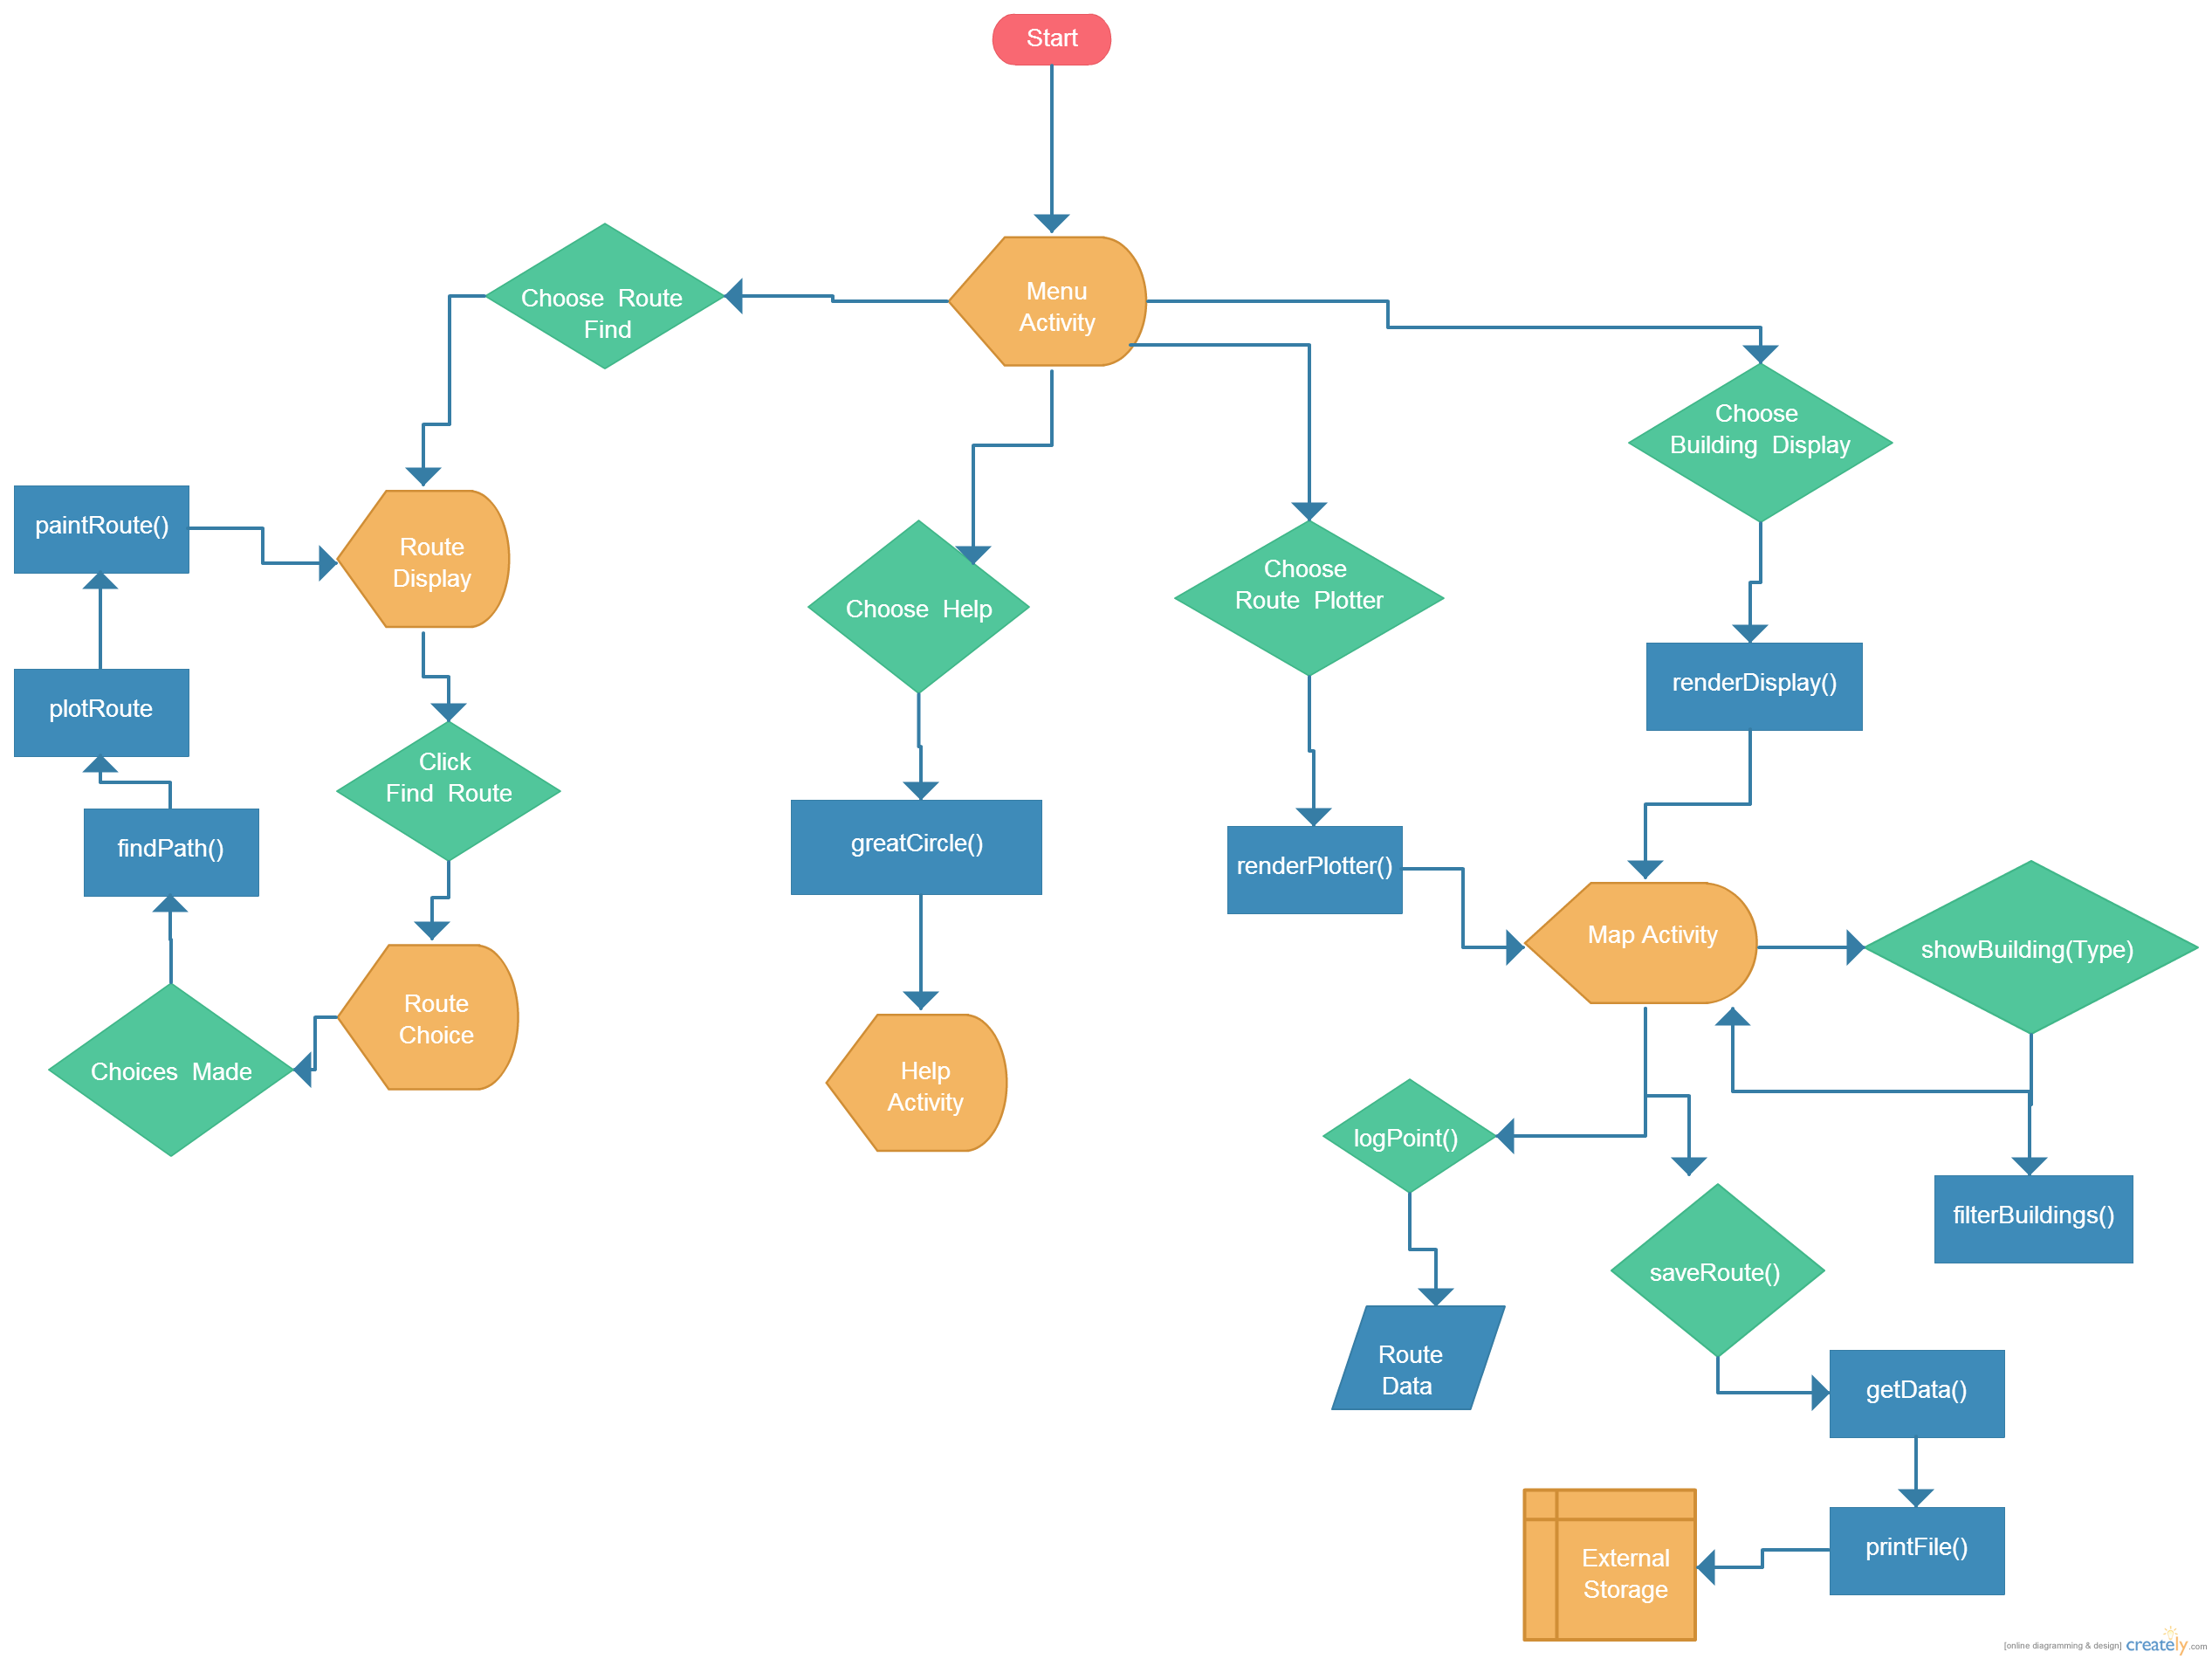
\includegraphics[scale=0.24]{Design/Flow.png}
\caption[Initial Flow Diagram]{Initial Flow Diagram depicting the path a user can follow through the application}
\end{sidewaysfigure}


\newpage
\restoregeometry
\subsection{Class Diagram}
The diagram on the following page describes the estimated architecture of the application, in following is the justification of the current estimated design.
\subsubsection{Justification}
The diagram begins at what is intended to be the root of the application, which branches out into the various activities. The simplest of these activities is the Help Activity, the Help activity has an ArrayList of Place, these represent the locations which will be loaded in through the loadHelpPoints() method. These will then have a distance assigned to them using the calcDist function before finally being sorted by the sortHelpPoints function. The closest will then be displayed using the displayClosest. While split up into several methods here it may be reasonable to merge a couple of them together, this will be decided upon implementation. 

The second activity is the Map activity, which will be rendered based on what the user wants. If the user wants a plotter the user will be able to log a point using logPoint which will be followed by connectPoints, causing a path to appear on the map. Finally the user will want to create a file so createFile will be called causing the creation of the File Printer class which will handle the formatting and output of the data into the correct directory. 

The Map Activity will also be responsible for rendering the view for the viewing of buildings based on filter, filter will be chosen by the user. The buildings will be loaded in using the loadPlaces function which will read the buildings in. A Place also can have a Categories represented by an Enumeration, by doing this it should be easy to put a filter in the showByType function which will then display different Categories based on what the user wants. 

The most complex piece of the diagram is probably the Route Display and its connecting classes. The activity has an ArrayList of Routes which will make up the entire path. This allows us to have different gradings along different parts of our final Paths. The Route Display class will start the Route Choose Activity for a result, in this case the result will be an ArrayList of Routes which will be contained within the returned Intent. 

The Route Choose activity has two expandable list views, which will be populated by the available nodes to travel to in the graph, not all nodes can be travelled to. The options chosen will then be taken and a search performed using the findPath function. The findPath function will return an ArrayList of Routes which will be put into the intent and the Route Display will be returned to.

On return to the Route Display Activity the onActivityResult will be run, which will grant access to the returned Intent object and remove the extras from it using the getRoute method. The path will then be set, which is really setting a possibly long list of smaller Routes. The poly lines used to set the Routes will also be coloured based on their grading. This will be displayed to the user and they will be able to move around the route and have their position displayed using methods native to the Google Maps Android API\cite{maps}. 

This design will be kept to as close as possible during development, due to the design being created in such a way that it provides the modular application we want to finish with. 
\begin{sidewaysfigure}
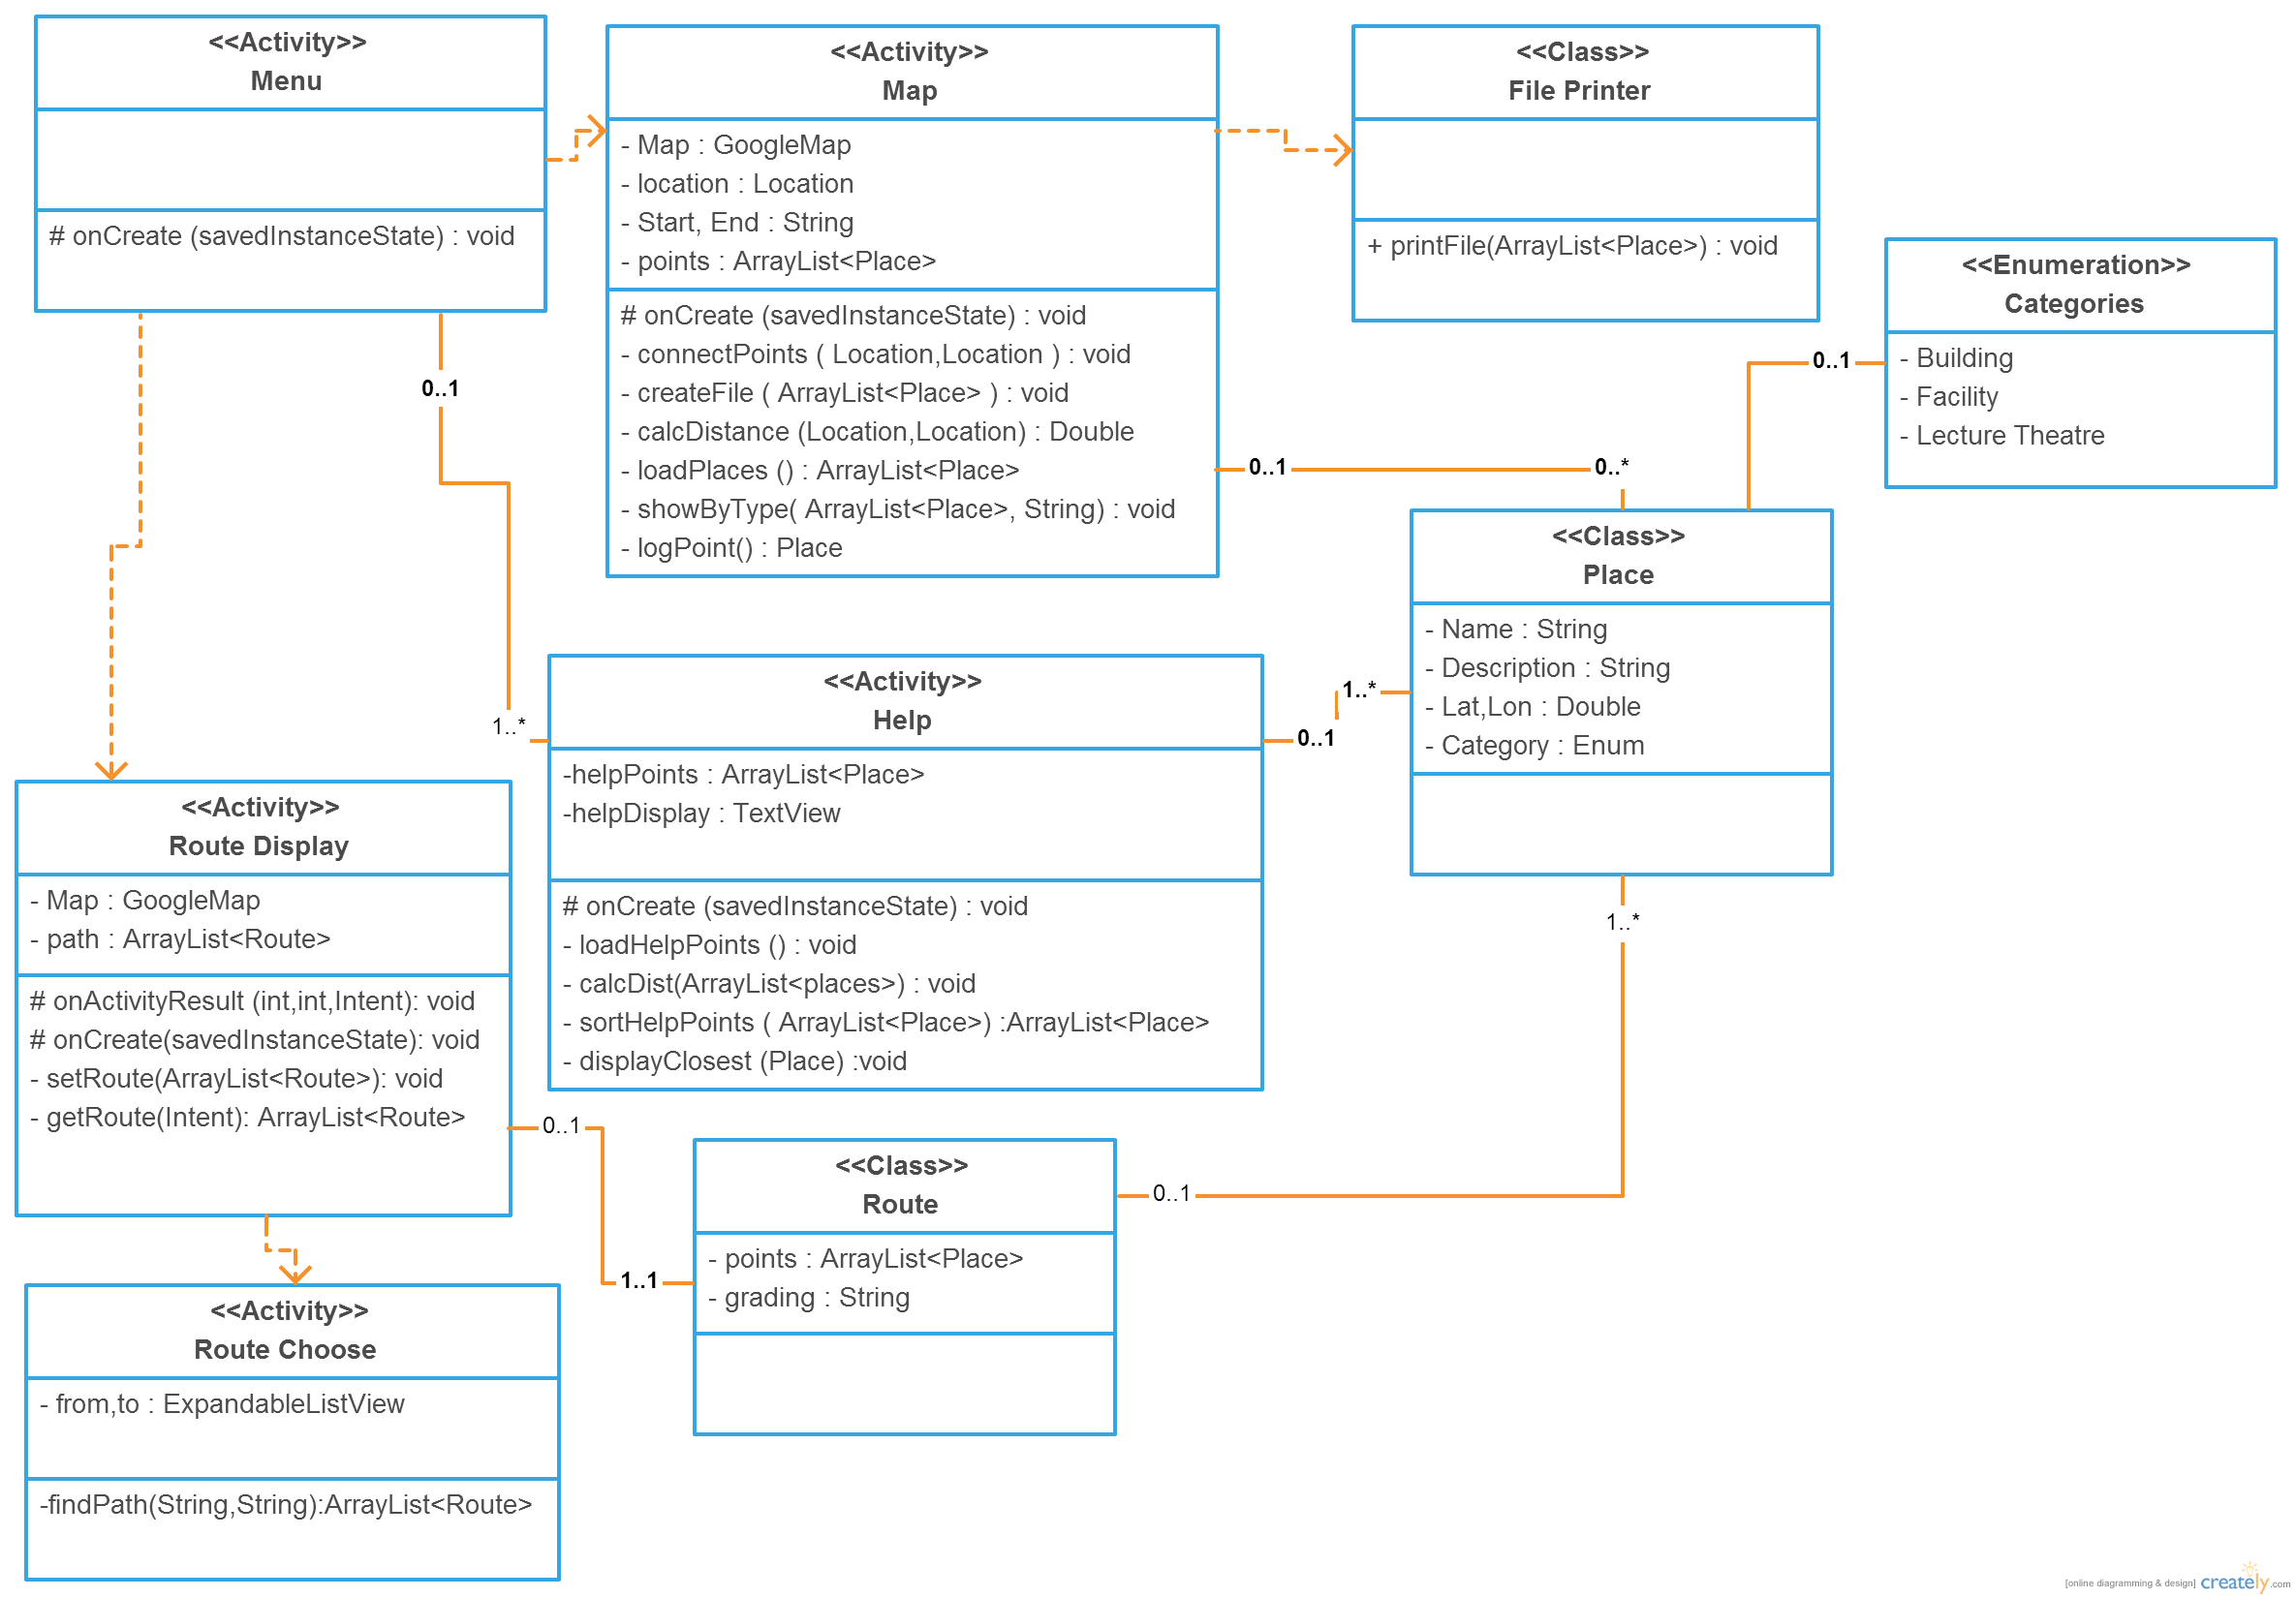
\includegraphics[scale=0.25]{Design/Class.png}
\caption[Initial Class Diagram]{Initial Class Diagram depicting the links between classes in UML notation}
\end{sidewaysfigure}
\newpage
\subsection{Screen Designs}
The following section will include information about the planned Screen Designs and the justification for the proposed designs. Overall the screens have been currently designed to match the colour scheme of the University and as such look as in fitting with the University as it can. It should not be too much problem to have the Screens very closely resemble the designs laid out. 

The button style used throughout the design images shown below will be a custom style written up in XML, various resources can be found on line for both colour picking and XML button design. 
\subsubsection{Menu Screen}
\begin{figure}[h]
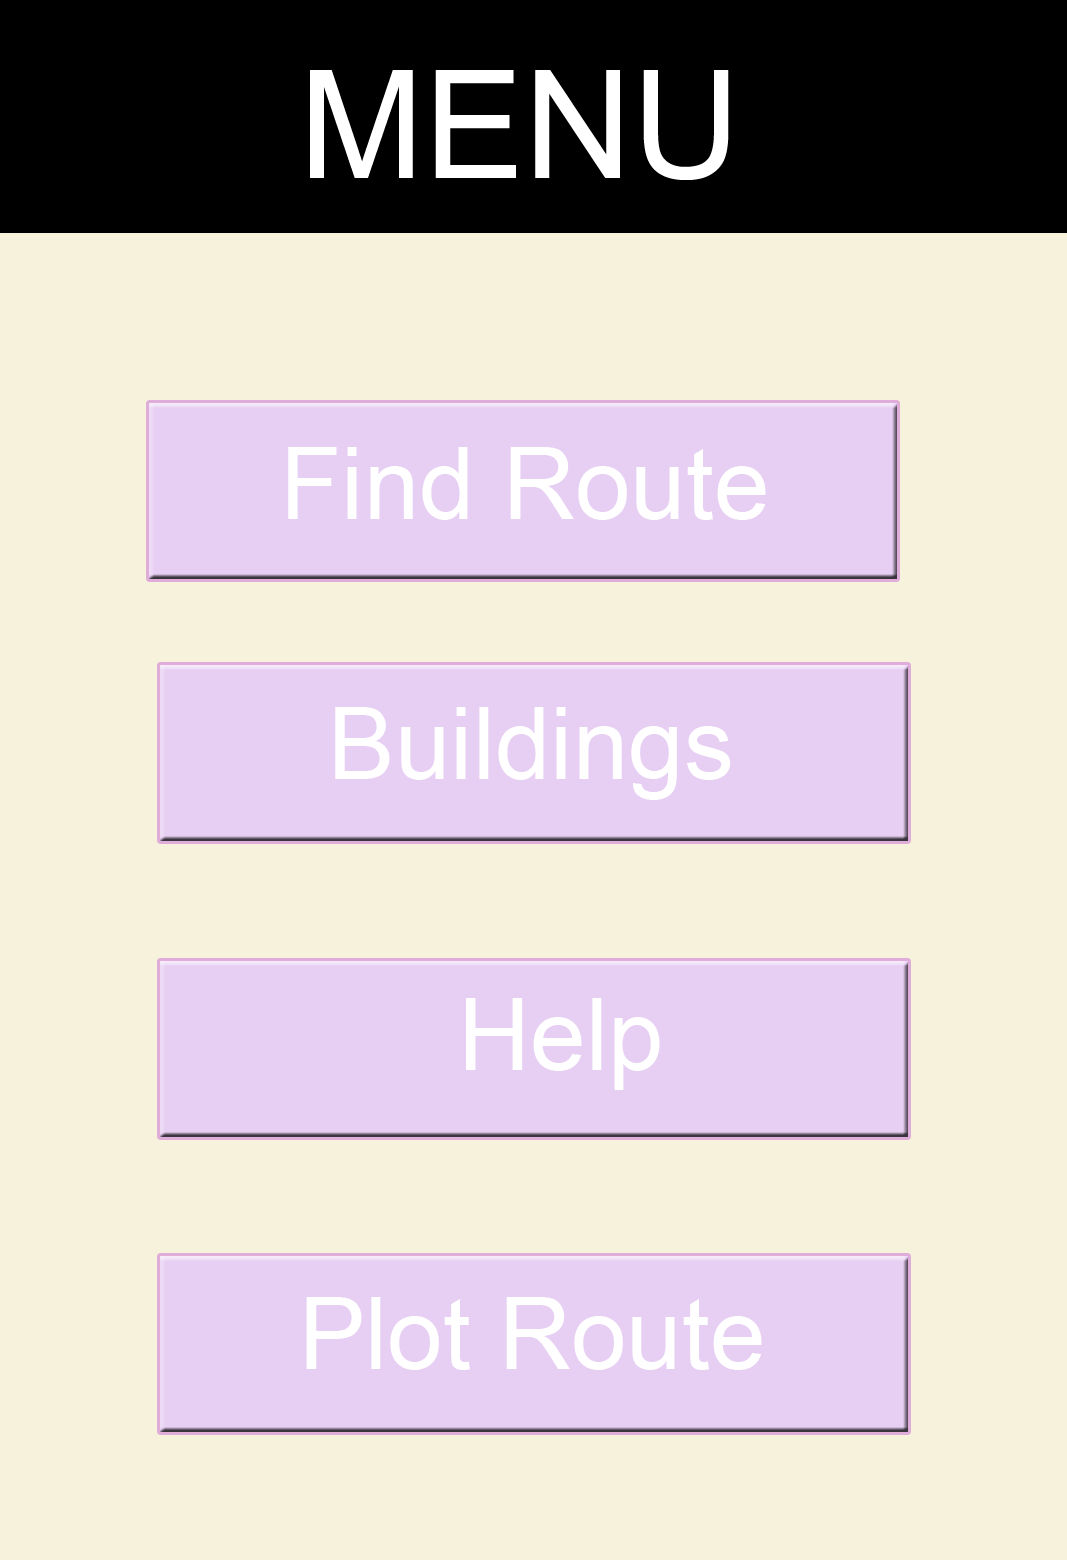
\includegraphics[scale=0.6]{Design/Menu.png}\\
\caption[Initial Menu Design]{Initial Menu Design depicting the predicted layout of the main screen.}
\end{figure}

As can be seen from the above diagram the user will have the label of the current page across the top of the activity, as is common within android applications. The options to move onto the connecting pages will then be arranged within a linear layout and have there respective linked activities as button text. Other options included horizontal buttons but with large screens it could look out of place and be too stretched.

Another possible choice was to have the screens swipe able, so all of the activities are essentially in a row. However after initial research the implementation of this could take long enough to slow down the development of some of the key features. Other possible choices included the inclusion of external libraries, especially some from the 'awesome-android-ui'\cite{aui} package, however it has been decided all design will be developed without the use of outside libraries. If time is available at the end of the projects time line it could be possible to try a test of this for future development. 
\subsubsection{Help Screen}
\begin{figure}[h]
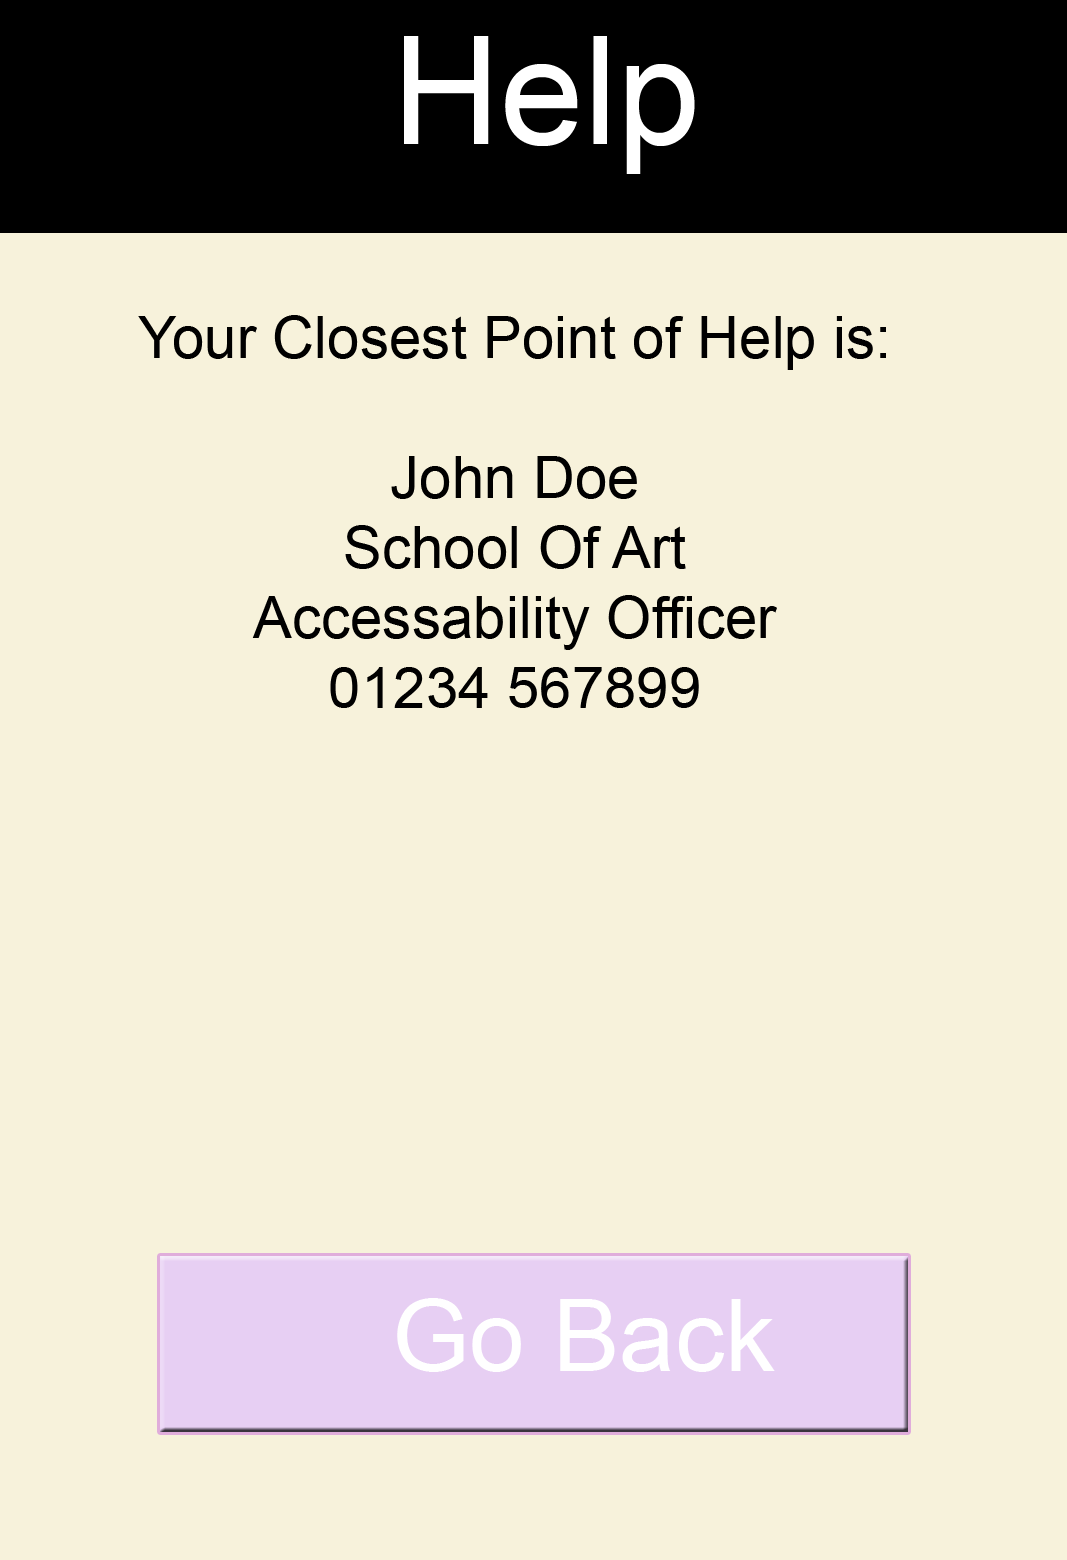
\includegraphics[scale=0.6]{Design/Help.png} \\
\caption[Initial Help Design]{Initial Design for the Help screen, displays information based on user location.}
\end{figure}
The Help screen is again a fairly simple design, the text shown will be a text view which contains the decided location with a button which takes the user back to the Menu Activity. 
\newpage
\subsubsection{Display Buildings}
\begin{figure}[h]
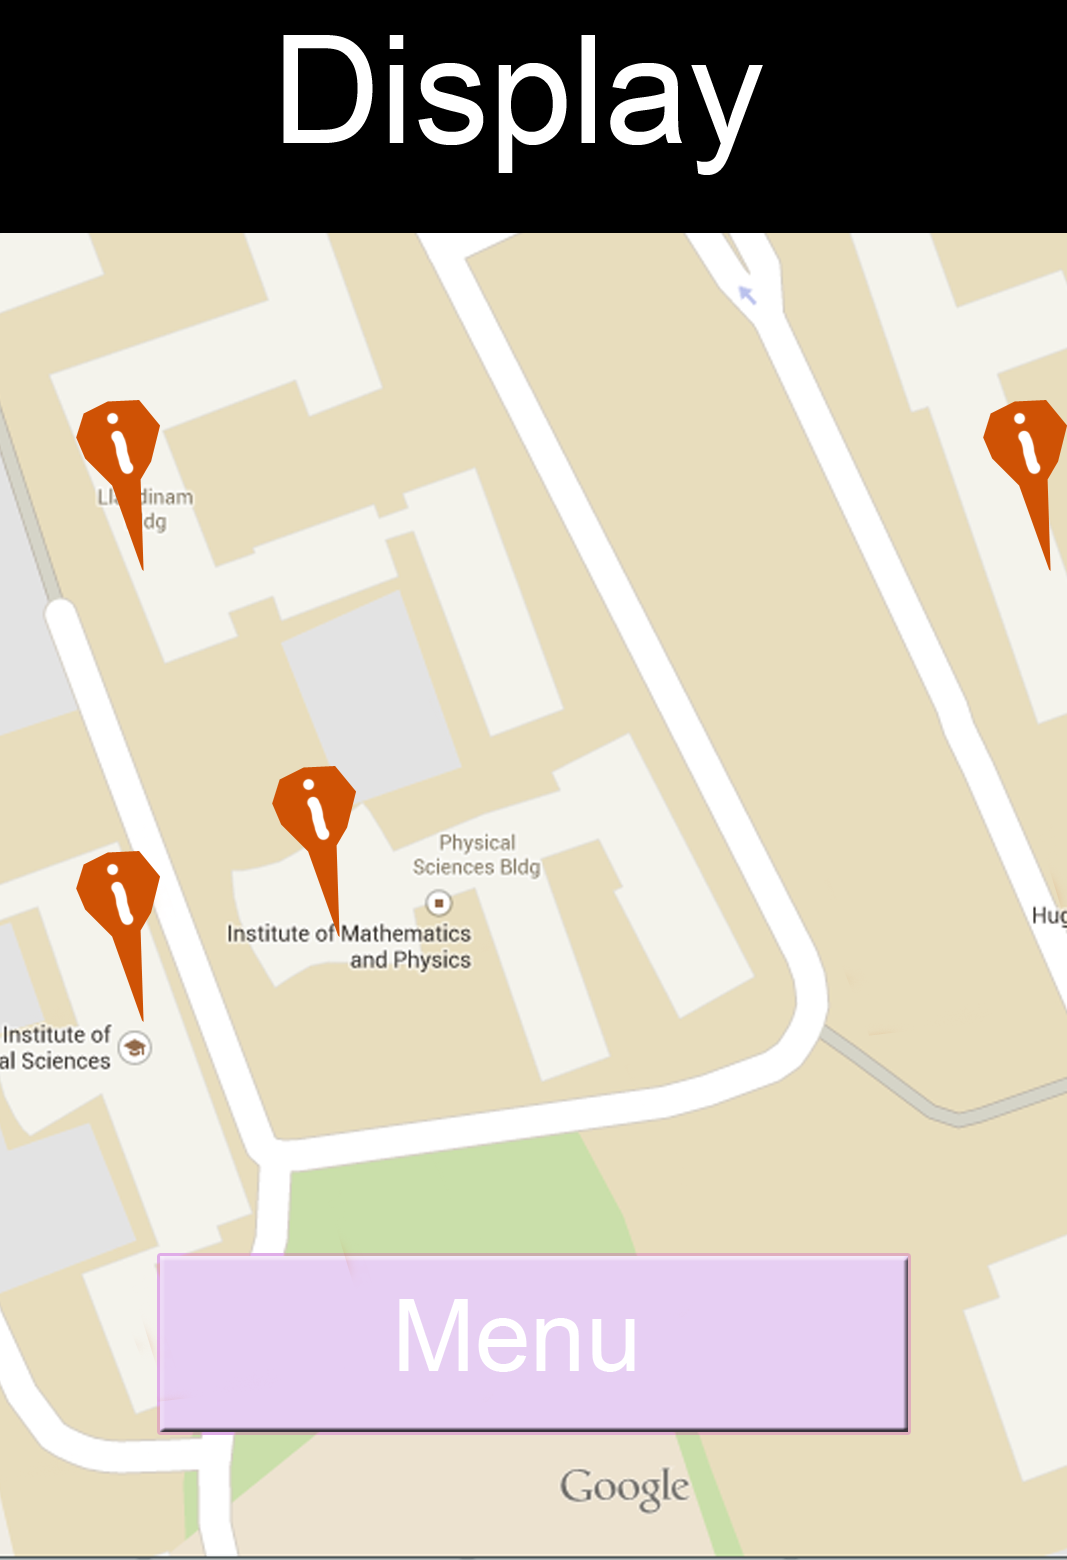
\includegraphics[scale=0.6]{Design/Display.png}\\
\caption[Initial Display Design]{Initial Display Design, view of buildings based on user filtered options.}
\end{figure}
The Display buildings screen will contain a Google Map and have a button which allows for the customisation of which types of buildings are shown. The Menu button will bring up a pop up menu which will allow users to set categories thus showing different markers and there relevant information. 
\newpage
\subsubsection{Route Plotter}
\begin{figure}[h]
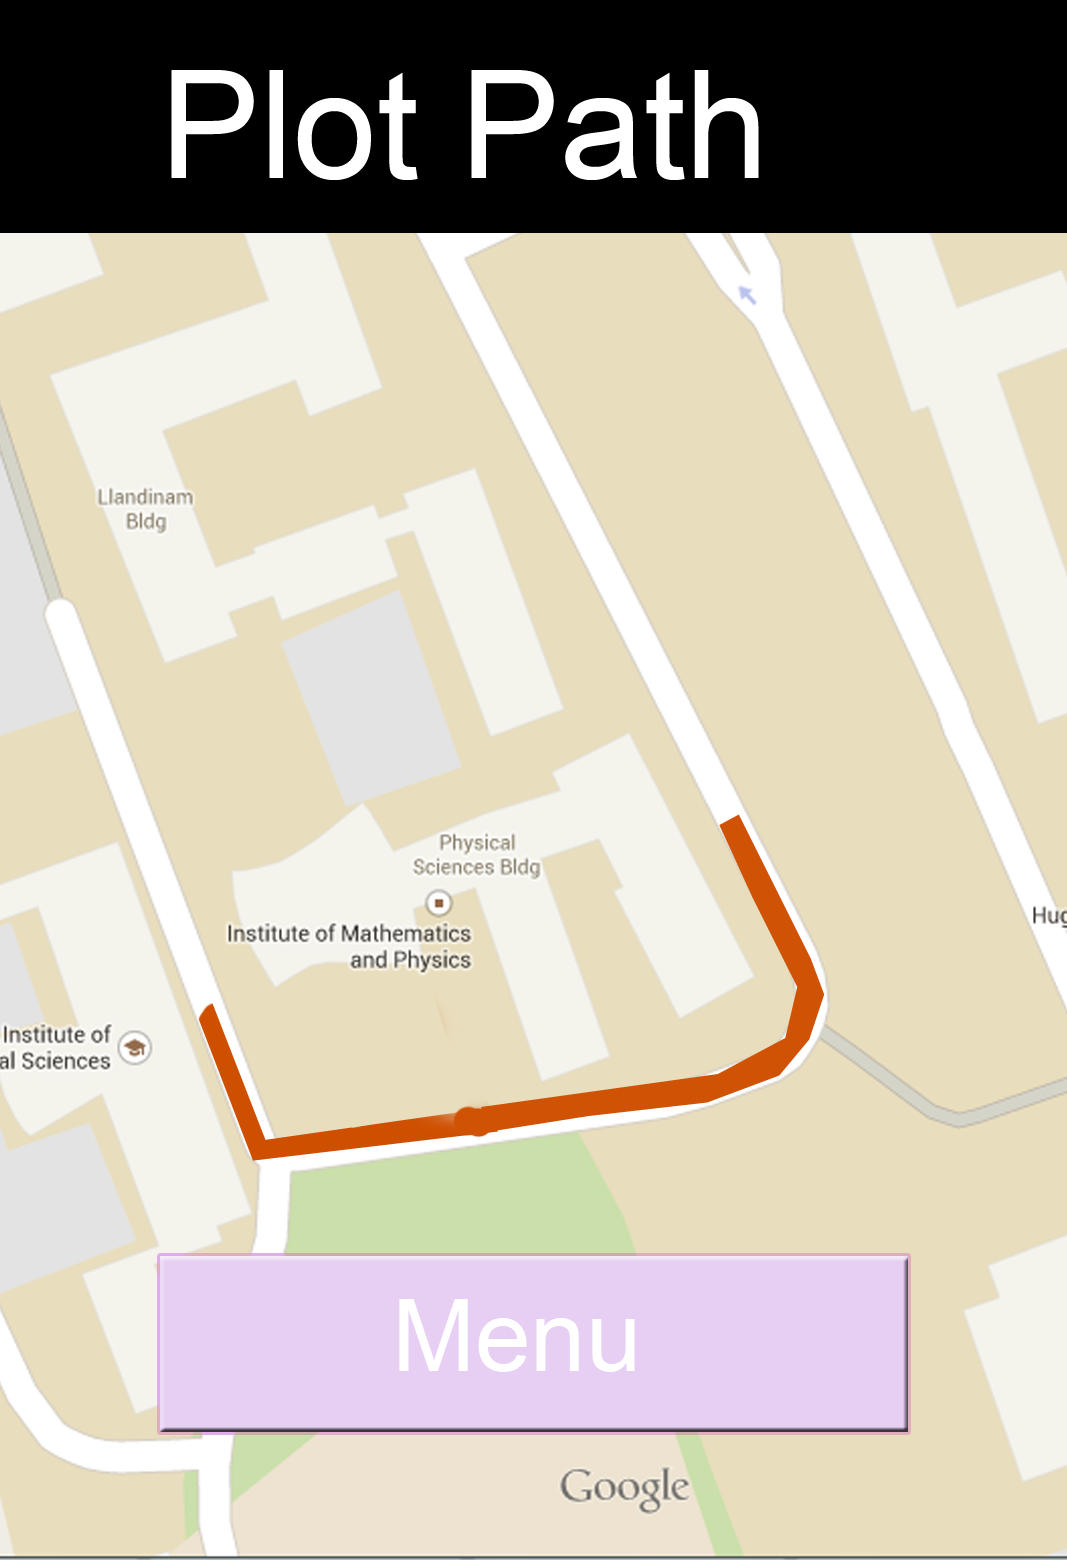
\includegraphics[scale=0.6]{Design/Plot.png}\\
\caption[Initial Plot Design]{Initial design for the route plotting screen for the use of future maintainers.}
\end{figure}
As can be seen from the design the screen will again hold a Menu button, with a pop up menu, which allows the user to choose from a range of options including loggings points, cancelling the current route and saving it to a file. It should also allow for incrementing steps on the route. The Route being walked can be shown on the screen through a use of a set of poly lines.
\newpage
\subsubsection{Route Display}
\begin{figure}[h]
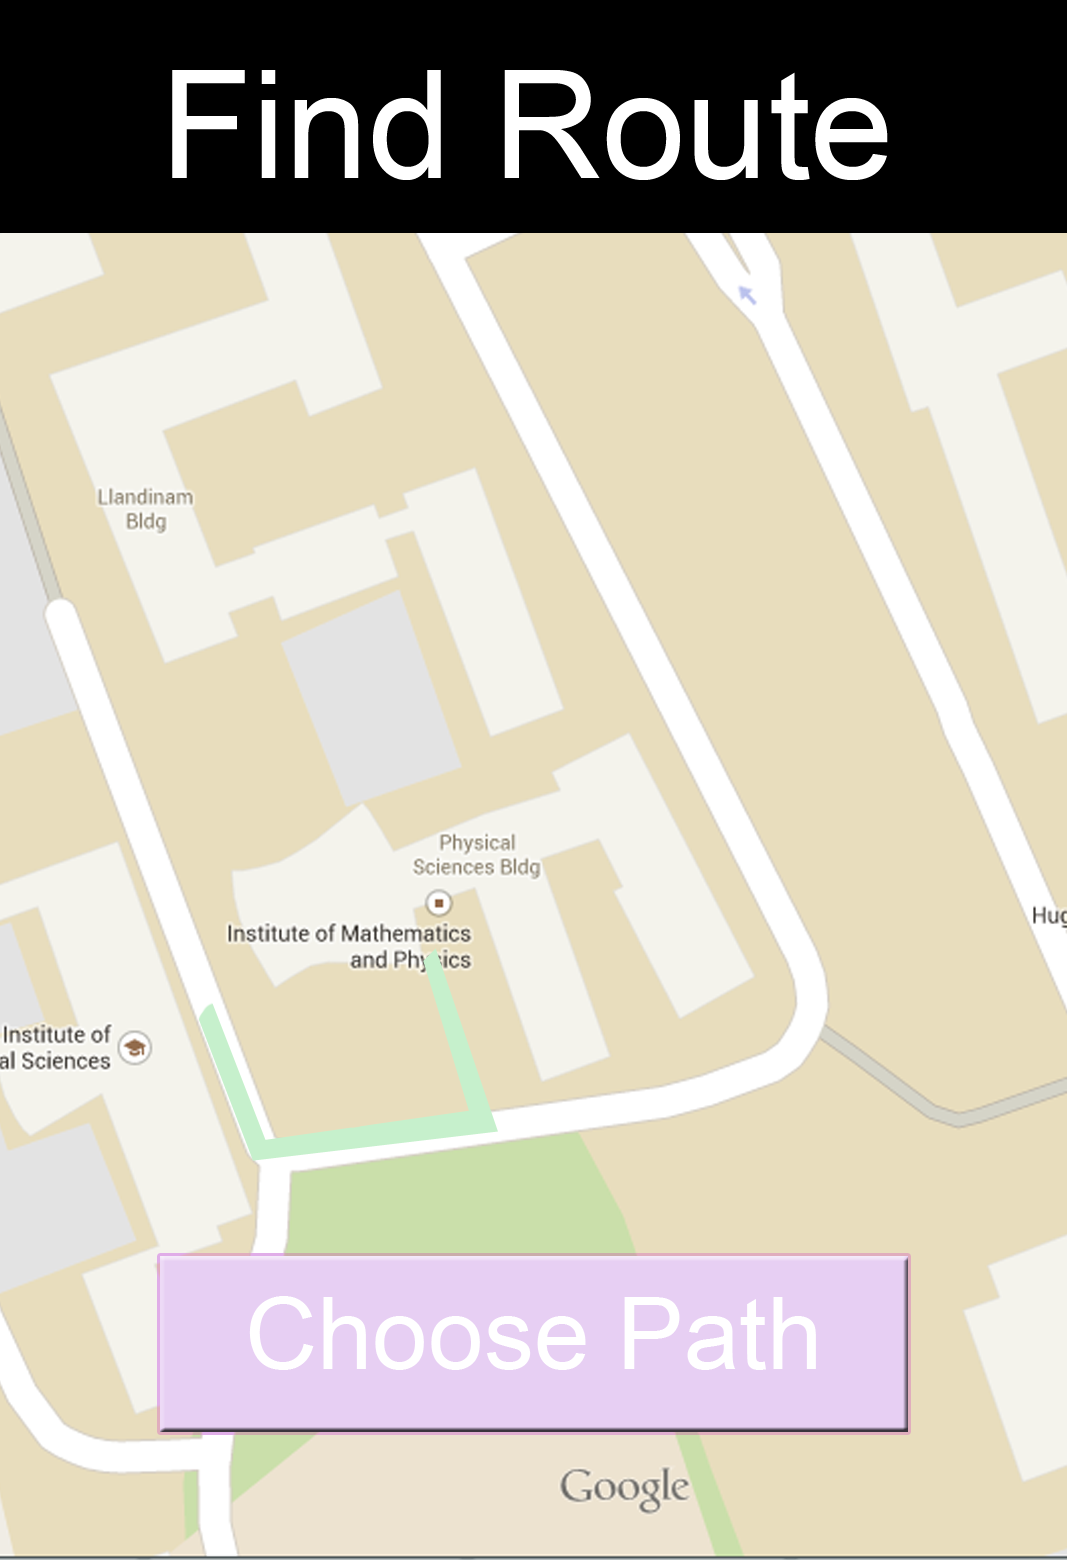
\includegraphics[scale=0.6]{Design/Route.png}\\
\caption[Initial Find Route]{Initial Design for the Route Display Screen including map object.}
\end{figure}
The Route display page the first time it is launched will hold nothing but the map object and a button, as no choice has been made. Afterwards however, as is shown here, the route will be displayed with different colours for segments that range in difficulty.
\newpage
\subsubsection{Route Choice}
\begin{figure}[h]
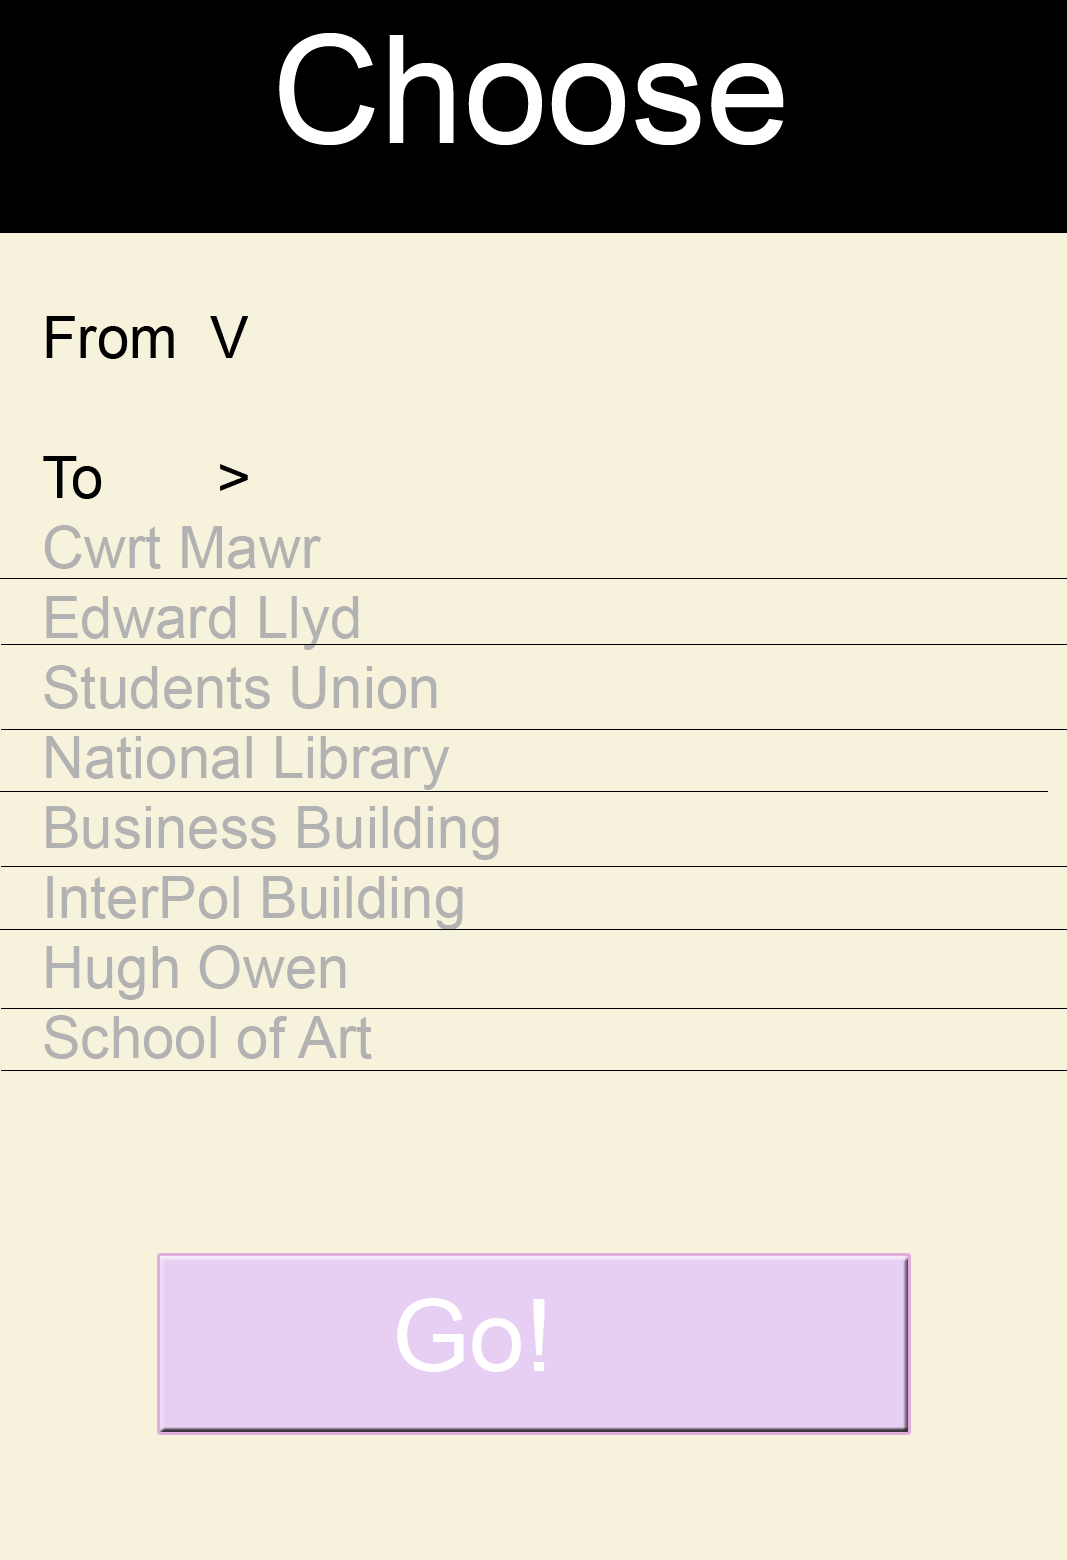
\includegraphics[scale=0.6]{Design/Choose.png}\\
\caption[Initial Route Choice Design]{Initial Screen Design for the Route Choice Activity}
\end{figure}
The final screen that will be included is the route choice screen, containing two expandable list views which will then add the chosen start and destination to the extras for the activity to be passed back. The Button this time will return the user to the Find Route screen which will display the chosen route. 
\subsubsection{Design Notes}
As can be seen the screens try to keep a very consistent style between them, it is felt this is necessary to provide the user with an intuitive experience. Especially in this application due to the criticisms that have been made about the Web version and our access to those criticisms. Other feedback will also be gathered from users meaning that this design could change once that has been gathered. Initial design feedback will be gathered once all screens are functional, it may not be necessary to finish features just their proposed layouts.



\fancypagestyle{plain}{%
   \fancyhead{} %[C]{Annotated Bibliography}
   \fancyfoot[C]{{\thepage} of \pageref{LastPage}} % except the center
   \renewcommand{\headrulewidth}{0pt}
   \renewcommand{\footrulewidth}{0pt}
}

\setemptyheader

\nocite{*} % include everything from the bibliography, irrespective of whether it has been referenced.

% the following line is included so that the bibliography is also shown in the table of contents. There is the possibility that this is added to the previous page for the bibliography. To address this, a newline is added so that it appears on the first page for the bibliography. 
\addcontentsline{toc}{chapter}{Annotated Bibliography} % Adds References to contents page

%
% example of including an annotated bibliography. The current style is an author date one. If you want to change, comment out the line and uncomment the subsequent line. You should also modify the packages included at the top (see the notes earlier in the file) and then trash your aux files and re-run. 
%\bibliographystyle{authordate2annot}
\bibliographystyle{IEEEannot}
\renewcommand{\bibname}{Annotated Bibliography} 
\bibliography{References/references} % References file


\end{document}
